%%%%%%%%%%%% 选择学位类型:专硕%%%%%%%%%%
\documentclass[EnMaster]{BJTU-thesis}  %%专硕
\usepackage[T1]{fontenc}  %设置英文字体为times new roman
\usepackage{mathptmx}
 

%%%%%%%%%%%%%%%%%填写封面信息%%%%%%%%%%%%%%%%%%%%%%%%
\author{饶欣宇}                                  %作者姓名
\studentNumber{22125303}                       %作者学号
\advisor{赵佳}                                 %导师姓名
\advisorTitle{副教授}                            %导师职称
\degreeType{工学}                              %学位类别
\major{计算机与信息技术学院}                         %所属专业
\researchArea{联邦学习与车联网}                        %研究方向
\title{基于联邦学习的车联网异常检测系统}                               %论文题目
\englishtitle{Anomaly Detection System for Internet of Vehicles based on Federated Learning}           %论文题目英文
\datetime{2024年6月}                           %编辑日期


%%%%%%%%%%%%%%%%%%%%%%%%%%%%%%%%%%%%%%%%%%%%%%
%\setmainfont{Times New Roman}

\begin{document}
	\makecover
	\makeAuthorization
	\makeInfo
	 \setlength{\baselineskip}{20pt}
\begin{thanks}
\noindent 放置在摘要页前,对象包括:1)国家科学基金,资助研究工作的奖学金基金,合同单位,资助或支持的企业、组织或个人。2)协助完成研究工作和提供便利条件的组织或个人。3)在研究工作中提出建议和提供帮助的人。4)给予转载和引用权的资料、图片、文献、研究思想和设想的所有者。5)其他应感谢的组织和个人。
\end{thanks} 									 %致谢部分
	\setlength{\baselineskip}{20pt}
\begin{abstract}
	[鼠标左键单击选择该段落,输入替换之。内容为小四号宋体。] 中文摘要应将学位论文的内容要点简短明了地表达出来,硕士学位论文一般为500~1000字,博士学位论文一般为1000~2000字。留学生英文版学位论文不少于3000字中文摘要,留学生英文版博士学位论文不少于5000字中文摘要。字体为宋体小四号。内容应包括工作目的、研究方法、成果和结论。要突出本论文的创新点,语言力求精炼。为了便于文献检索,应在本页下方另起一行注明论文的关键词(3-8个),如有可能,尽量采用《汉语主题词表》等词表提供的规范词。图X幅,表X个,参考文献X篇。
		
	\noindent\keywords{你好;世界}
\end{abstract}   								 %中文摘要
	 \setlength{\baselineskip}{20pt}
\begin{englishabstract}
	English Abstract.English Abstract.English Abstract.English Abstract.English Abstract.English Abstract.English Abstract.English Abstract.English Abstract.English Abstract.English Abstract.English Abstract.English Abstract.English Abstract.English Abstract.English Abstract.English Abstract.English Abstract.English Abstract.English Abstract.English Abstract.
	
	\noindent\englishkeywords{Hello; World}
\end{englishabstract}  							 %英文摘要
      \setlength{\baselineskip}{20pt}
\begin{preface}
	[鼠标左键单击选择该段落,输入替换之。内容为小四号宋体。] 学位论文的序或前言,一般是作者或他人对本篇论文基本特征的简介,如说明研究工作缘起、背景、主旨、目的、意义、编写体例,以及资助、支持、协作经过等;也可以评述和对相关问题发表意见。这些内容也可以在正文引言中说明。
		
	
\end{preface}                                             %序言

	
	
	\tableofcontents
     \newpage\pagenumbering{arabic}

     %正文部分
 %     \setlength{\baselineskip}{20pt}
\chapter{引言}
\label{cha:intro}

% [鼠标左键单击选择该段落,输入替换之。内容为小四号宋体。] 引言(或绪论)简要说明研究工作的目的、范围、相关领域的前人工作和知识空白、理论基础和分析、研究设想、研究方法和实验设计、预期结果和意义等。应言简意赅,不要与摘要雷同,不要成为摘要的注释。一般教科书中有的知识,在引言中不必赘述。

\section{研究背景和意义}

车联网(Internet of Vehicles,IoV)是一种基于物联网(Internet of Things,IoT)技术的智能交通系统,它通过车辆、电子、信息通信、道路交通运输等行业的深度融合,构建了一个由各种设备和异构网络组成的全球网络\cite{Architecture_Protocols_and_Security_in_IoV}。车联网是实现智能出行、智慧城市、智能物流等多种应用场景的关键技术,具有广泛的社会效益和经济价值。车联网是智能交通系统的基础和核心技术,通过车与车、车与路边单元两种通信模式,实现了移动车辆的实时感知、交通信息的协同和无线通信,提高了道路交通的安全性和效率。智能车联网不仅能够为车与车之间的间距提供保障,降低车辆发生碰撞事故的概率,还可以帮助车主实时导航与信息接收发送,通过与其他车辆和网络系统的通信实现道路环境预警。近年来,智能车联网迎来了高速发展的时代,各大汽车公式和互联网厂商都在竞相研发自动驾驶技术\cite{ref1},将车辆作为物联网的智能节点\cite{ref2}并利用无线传感器网络(WSN)实现车辆和路边设备的互联。2021年,《国家综合立体交通规划纲要》发布,将智能网联汽车、智慧交通基础设施建设作为重点任务,展现了对智能车联网的重视和支持。

然而,智能车联网也面临着严峻的网络安全挑战,因为智能网联车辆的架构日益复杂,涉及车辆、人类和其他智能设备或物品等多种网络资源\cite{Attacks_and_countermeasures_in_the_internet_of_vehicles,Attack_IOV2},车辆也集成了多种自动驾驶功能、通信接口和传感器。车端的车载网络由控制器局域网(CAN),本地互连网络(LIN),家用数字总线,FlexRay,以太网,面向媒体的系统传输,接口描述块和低压差分信号等多种异构网络组成\cite{Cybersecurity_for_autonomous_vehicles_Review_of_attacks_and_defense},这就导致了冒充攻击、GPS欺骗攻击、重放攻击、窃听攻击等安全问题在智能网联汽车上的出现\cite{ref3,ref4,Architecture_Protocols_and_Security_in_IoV},如图\ref{fig:Vehicle_networking_architecture}所示。例如,攻击者可能会通过车辆的蓝牙漏洞实现对车载网络的访问,进而控制制动等功能。因此,汽车网络安全研究需要对汽车的设计、架构、功能、攻击面有一个宏观性的理解。由于传统的网络安全研究人员往往都没有参与过汽车的设计、研发、生产,对于汽车的了解仅限于其表面的功能表现,而汽车又是当今最复杂的工业制造产品之一,因此车联网安全是当今的研究热点。为了保障智能网联汽车的安全性和可靠性,本文从网络安全的角度,分析智能车联网的安全需求、安全威胁和安全防护,提出了一套针对车联网的安全解决方案,旨在为智能车联网的发展和应用提供理论和技术支持。

\begin{figure}[htb]
    \centering
    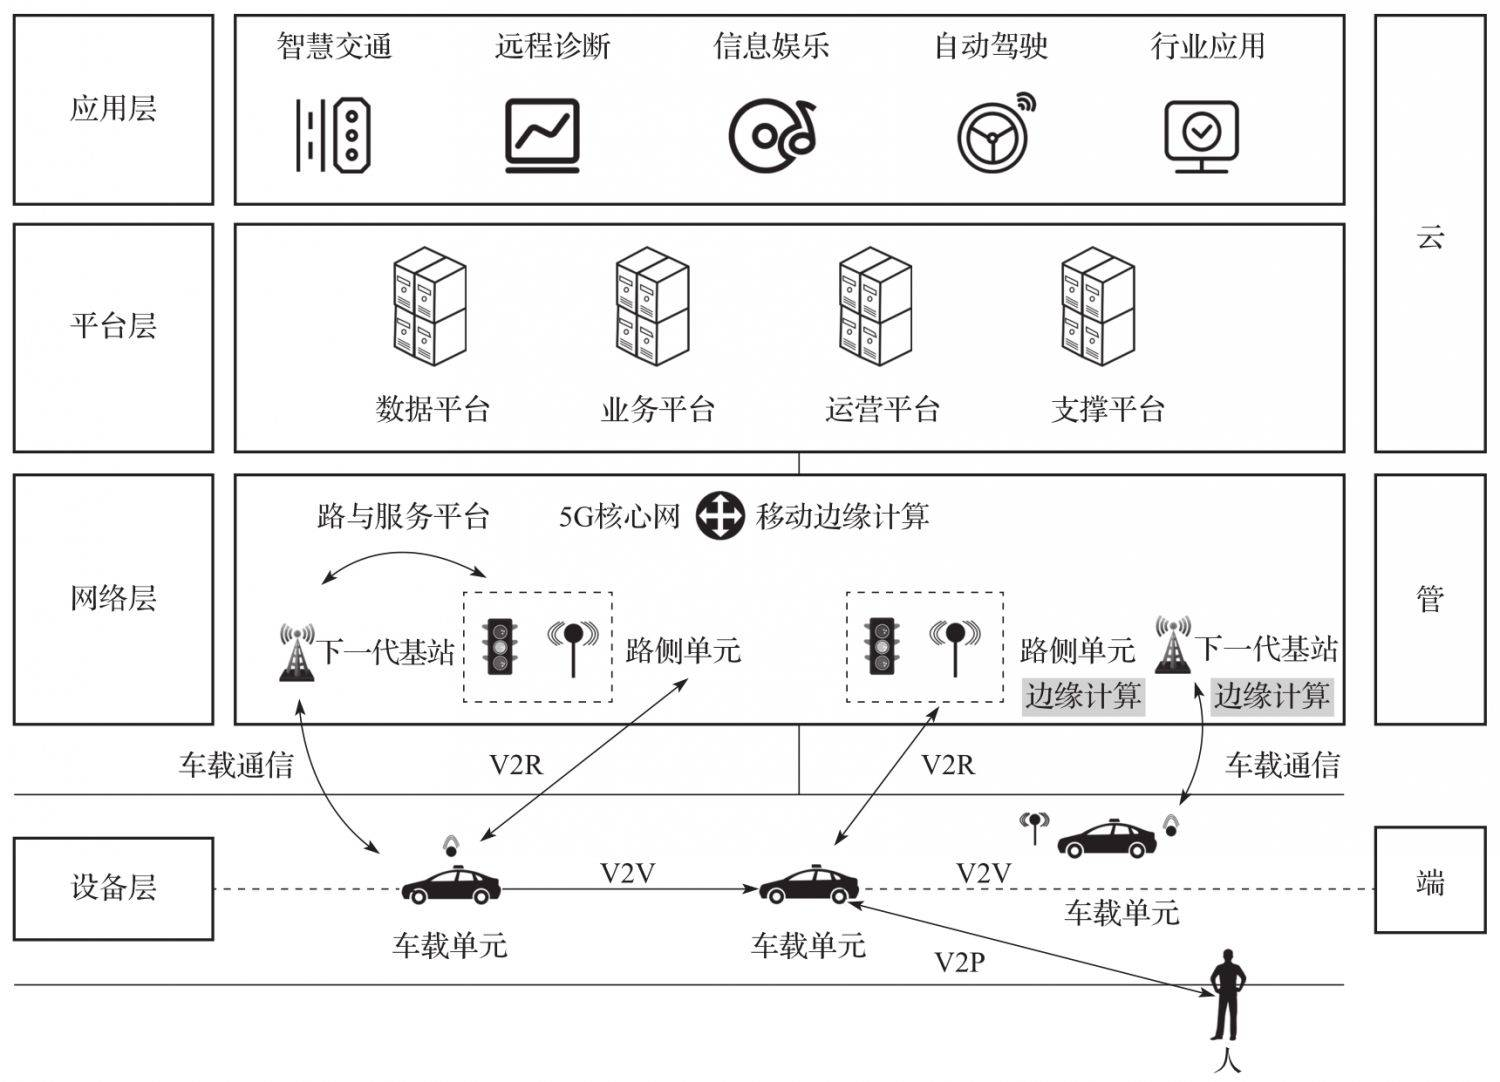
\includegraphics[width=0.95 \textwidth]{figures/chapter1/chapter1.4.jpg}
    \caption{从网络安全角度分析车联网架构}
    \label{fig:Vehicle_networking_architecture}
\end{figure}

当今时代,汽车行业没有出于安全原因限制互联网连接,反而出于商业原因继续增加互联网连接,在没有充分安全保障的情况下将新设备和新功能匆忙推向市场。同时,汽车系统里使用了大量无法保证安全性的开源软件,这使安全问题进一步加剧。英特尔的一项研究表明,如果只考虑自动驾驶专用传感器,仅一辆自动驾驶汽车每天就会产生大约4000GB的数据,每年产生的数据量更是惊人。汽车中的数据生成和收集并不是一个新现象。例如,为了有助于分析碰撞或技术故障,制造商需要记录事件数据和车载诊断数据。欧洲要求于2022年3月起新车强制安装EDR,存量车于2024年3月起安装。这些设备应该通过匿名存储事故数据来确定事故发生的原因,为事后调查提供数据支撑,类似于飞机上的黑匣子。过去几年的技术进步导致汽车收集的数据量和种类激增。汽车不仅是将驾驶员和乘客从A点带到B点的交通工具,而且也是一种智能设备,所以将装有传感器的汽车放在道路上存在隐私问题。汽车不仅会收集驾驶员和乘客的信息,还会收集周围的车辆、行人和城市的信息以及国家测绘数据。车联网中的数据隐私泄露与攻击行为不仅会侵犯车主和乘客的个人隐私,还会危害国家安全和社会稳定。例如,如果攻击者能够获取车辆的位置、速度、行驶路线等信息,就可能对车辆进行跟踪、拦截、劫持等恶意行为;如果攻击者能够获取车辆的控制权,就可能对车辆进行篡改、破坏、制造事故等恶意行为;如果攻击者能够获取车辆的通信内容,就可能对车辆进行监听、干扰、欺骗等恶意行为。这些恶意行为不仅会威胁车辆的正常运行,还会危害车主和乘客的生命财产安全,甚至会影响整个交通系统的稳定性。因此,本文将针对车联网的数据隐私泄露与攻击行为提出相应的保护措施。

车联网中广泛应用了深度学习(DL)模型,以提升车辆的智能化和个性化。例如,通过摄像头或者雷达等传感器,对车辆周围的道路环境进行识别,帮助车辆实现自动驾驶、车道保持、碰撞预警等功能的模型,如YOLO、Mask R-CNN、LaneNet等;通过语音或者手势等方式,与车主或者乘客进行交互,提供娱乐、导航、信息等服务的模型,如Alexa、Siri、斑马智行等;通过无线网络,与其他车辆或者路边设备进行通信,实现数据的交换和协同,提高车辆的安全性和效率,实现智能交通和车队管理等功能的模型,如V2X、C-V2X、DSRC等。然而,DL模型的性能依赖于训练数据集的规模和质量,而训练数据集中可能包含大量的敏感信息,攻击者可以通过逆向手段还原出训练数据集,从而泄露用户隐私。例如,公安机关发布的犯罪嫌疑人识别模型,其训练数据集包含了全国人口的图像信息,如果攻击者能够还原出训练数据集中的图像,就会暴露个人敏感信息。因此,如何在保护个人敏感信息的同时,提高数据的可用性,是DL应用面临的一个主要问题,也是DL未来发展和应用的一个重要因素。本文针对车联网中的隐私安全问题,提出了一种基于联邦学习的车联网异常检测方法,将车联网中的隐私安全分为数据安全与模型安全两部分。数据安全主要涉及车联网中的数据采集、存储、传输和处理过程中的隐私保护,包括数据的加密、匿名化、脱敏等技术。模型安全主要涉及车联网中的DL模型的训练、部署和使用过程中的隐私保护,包括模型的加密、混淆、防篡改等技术。数据安全和模型安全是车联网中的隐私安全的两个重要方面,缺一不可。

% \begin{figure}[htb]
%     \centering
%     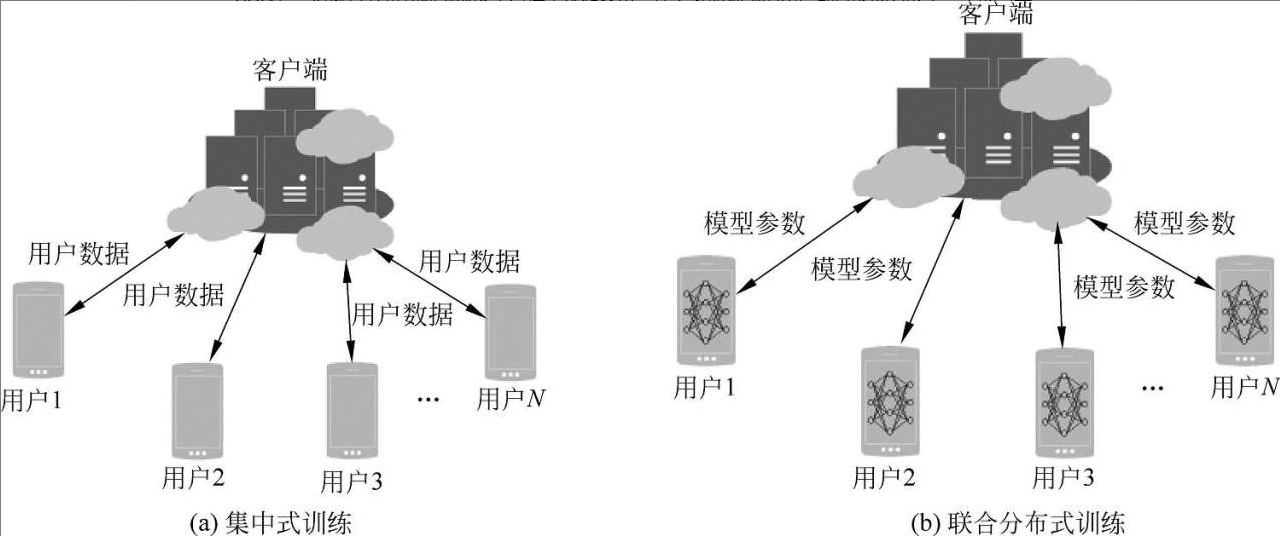
\includegraphics[width=0.85 \textwidth]{figures/chapter1/chapter1.1.png}
%     \caption{协作学习的两种威胁模型}
%     \label{fig:Two_threat_models_of_collaborative_learning}
% \end{figure}

% 将协作性模型与DL结合起来,可以通过多个数据源之间的协作来训练更加精确的协作性DL模型,在保证不同企业之间数据独立性的基础上,不同的企业之间可以实现模型的共享,任何一个模型学习到的知识都可以及时地共享给其他协作的企业,使所有企业都能从中受益。然而,协作性模型仍然会面临模型反演攻击、污染攻击等隐私窃取攻击的威胁。同时,一些领域对数据机密性的要求较高,比如在网络空间安全领域,如果遭受攻击,像入侵检测中用到的流量数据,会暴露目标网络的一些重要的配置信息;网站的请求数,会暴露网站架构以及用户的一些敏感隐私内容,同时,DL模型会无意中记录一些训练数据,而一些训练数据涉及人们的隐私,如习惯、爱好、地理位置等。在DL模型应用的健康系统中,隐私威胁不仅泄露患者隐私,攻击者可能发起攻击修改患者的用药剂量导致患者生命危险。因此安全厂商对于数据的机密性保护给予了高度重视。图\ref{fig:Deep_learning_model_training_methods}给出了常见的隐私窃取方式,这些隐私威胁分别针对机器学习过程中的训练阶段和预测阶段。
% \begin{figure}[htb]
%     \centering
%     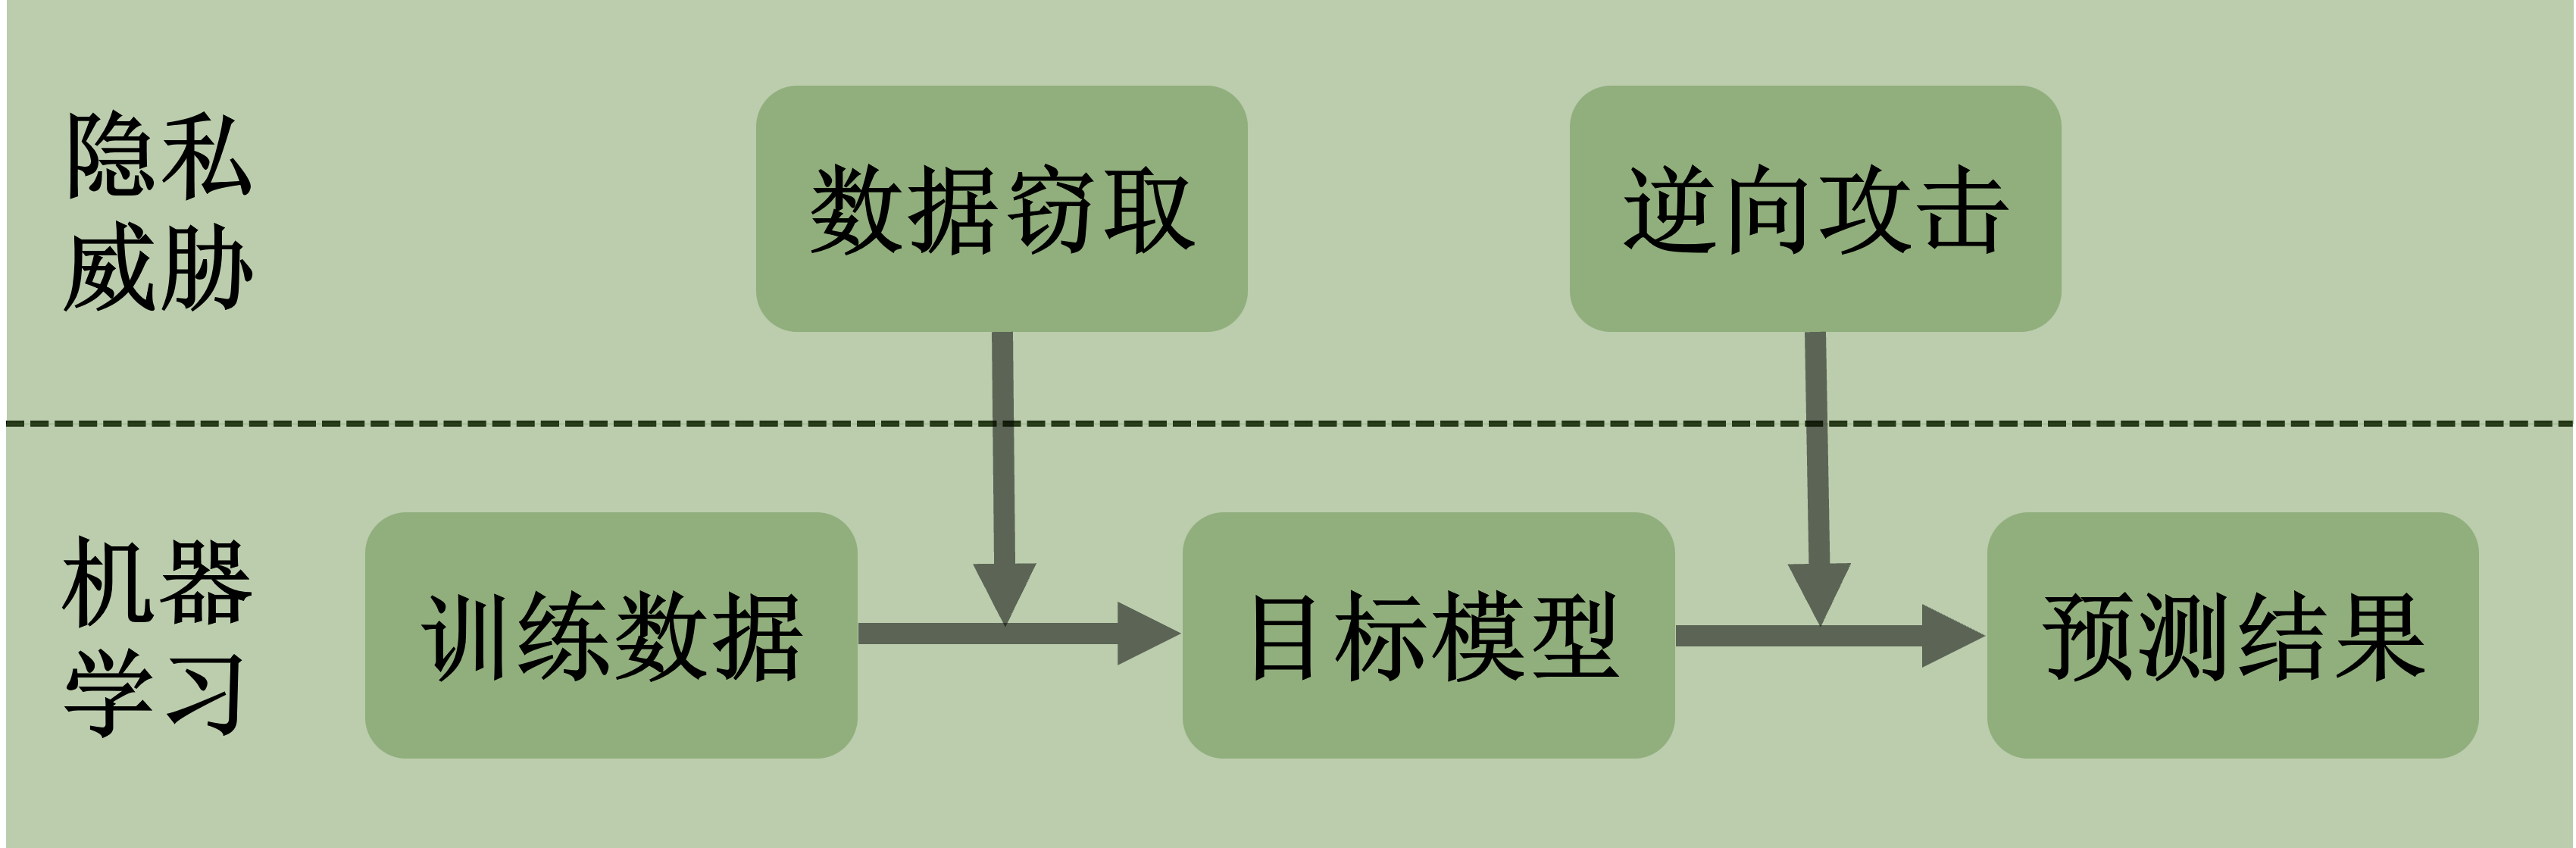
\includegraphics[width=0.55 \textwidth]{figures/chapter1/chapter1.png}
%     \caption{深度学习模型训练方式}
%     \label{fig:Deep_learning_model_training_methods}
% \end{figure}

% 传统的机器学习模式要求在模型训练之前将数据汇总到中心。但是,当数据偏离原有的数据域后,数据可能会变得无法控制,从而导致数据隐私泄露和数据安全风险。联邦学习是谷歌提出的一种分布式机器学习技术。与传统的机器学习不同,它不需要将数据集中在单个中心,从而支持分布式协作训练模型和保护数据隐私。由于其保护隐私和去中心化的内在特点,FL得到了各行各业的广泛青睐。对于大规模深度神经网络训练,联邦学习最近已成为分布式随机优的常见实现\cite{Gradient_Leakage_Attacks_in_Federated_Learning}。然而,大量研究表明联邦学习仍然存在大量安全问题,例如投毒攻击、对抗性样本攻击、隐私泄露等。在隐私泄露中,除了窃取模型之外,还可以从联邦训练中收集统计信息\cite{Safeguard_the_Original_Data_in_Federated_Learning_via_Data_Decomposition}。机器学习训练方式分为集中式和联合分布式,如图4-6所示。大型公司多用集中训练方式,因为拥有足够多的用户便于搜集大量的训练数据。在搜集用户数据过程中,会暴露一些用户的隐私,Google和Apple公司采用差分隐私的方式保护用户数据,在用户数据中,加入噪声使单一的数据没有现实意义,而统计信息具有应用价值。为了扩大训练数据集得到精确的目标模型,一些数据提供方需要进行协作“分享”数据,共同训练目标模型。“分享”不是直接对其他参与方公开数据,各个参与方独自在各自数据集上训练自己的模型,与其他参与方共享训练结果,从而间接分享各自的训练数据。

\section{研究内容及贡献}

本文旨在利用隐私保护策略,提高车联网中数据和模型的安全性,设计并实现了一种基于CAN总线的异常检测系统和一种基于稀疏学习和梯度扰动的梯度泄露防护方案。基于联邦学习的车联网异常检测系统的研究内容框架如图\ref{fig:Anomaly_detection_system_of_IoVFL}所示。本文的研究内容分为两个部分:第一部分是基于联邦学习的车联网CAN异常检测,通过构建多方参与的联邦学习模型,实现对车辆行驶状态的实时监测和异常识别;第二部分是基于稀疏学习和梯度扰动的梯度泄露防护方案,通过引入稀疏约束和随机扰动,降低联邦学习中梯度信息的可逆性和可推断性,保护参与者的隐私数据。下面将对将对数据安全和隐私保护的研究内容进行详细的介绍。

\begin{figure}[htb]
    \centering
    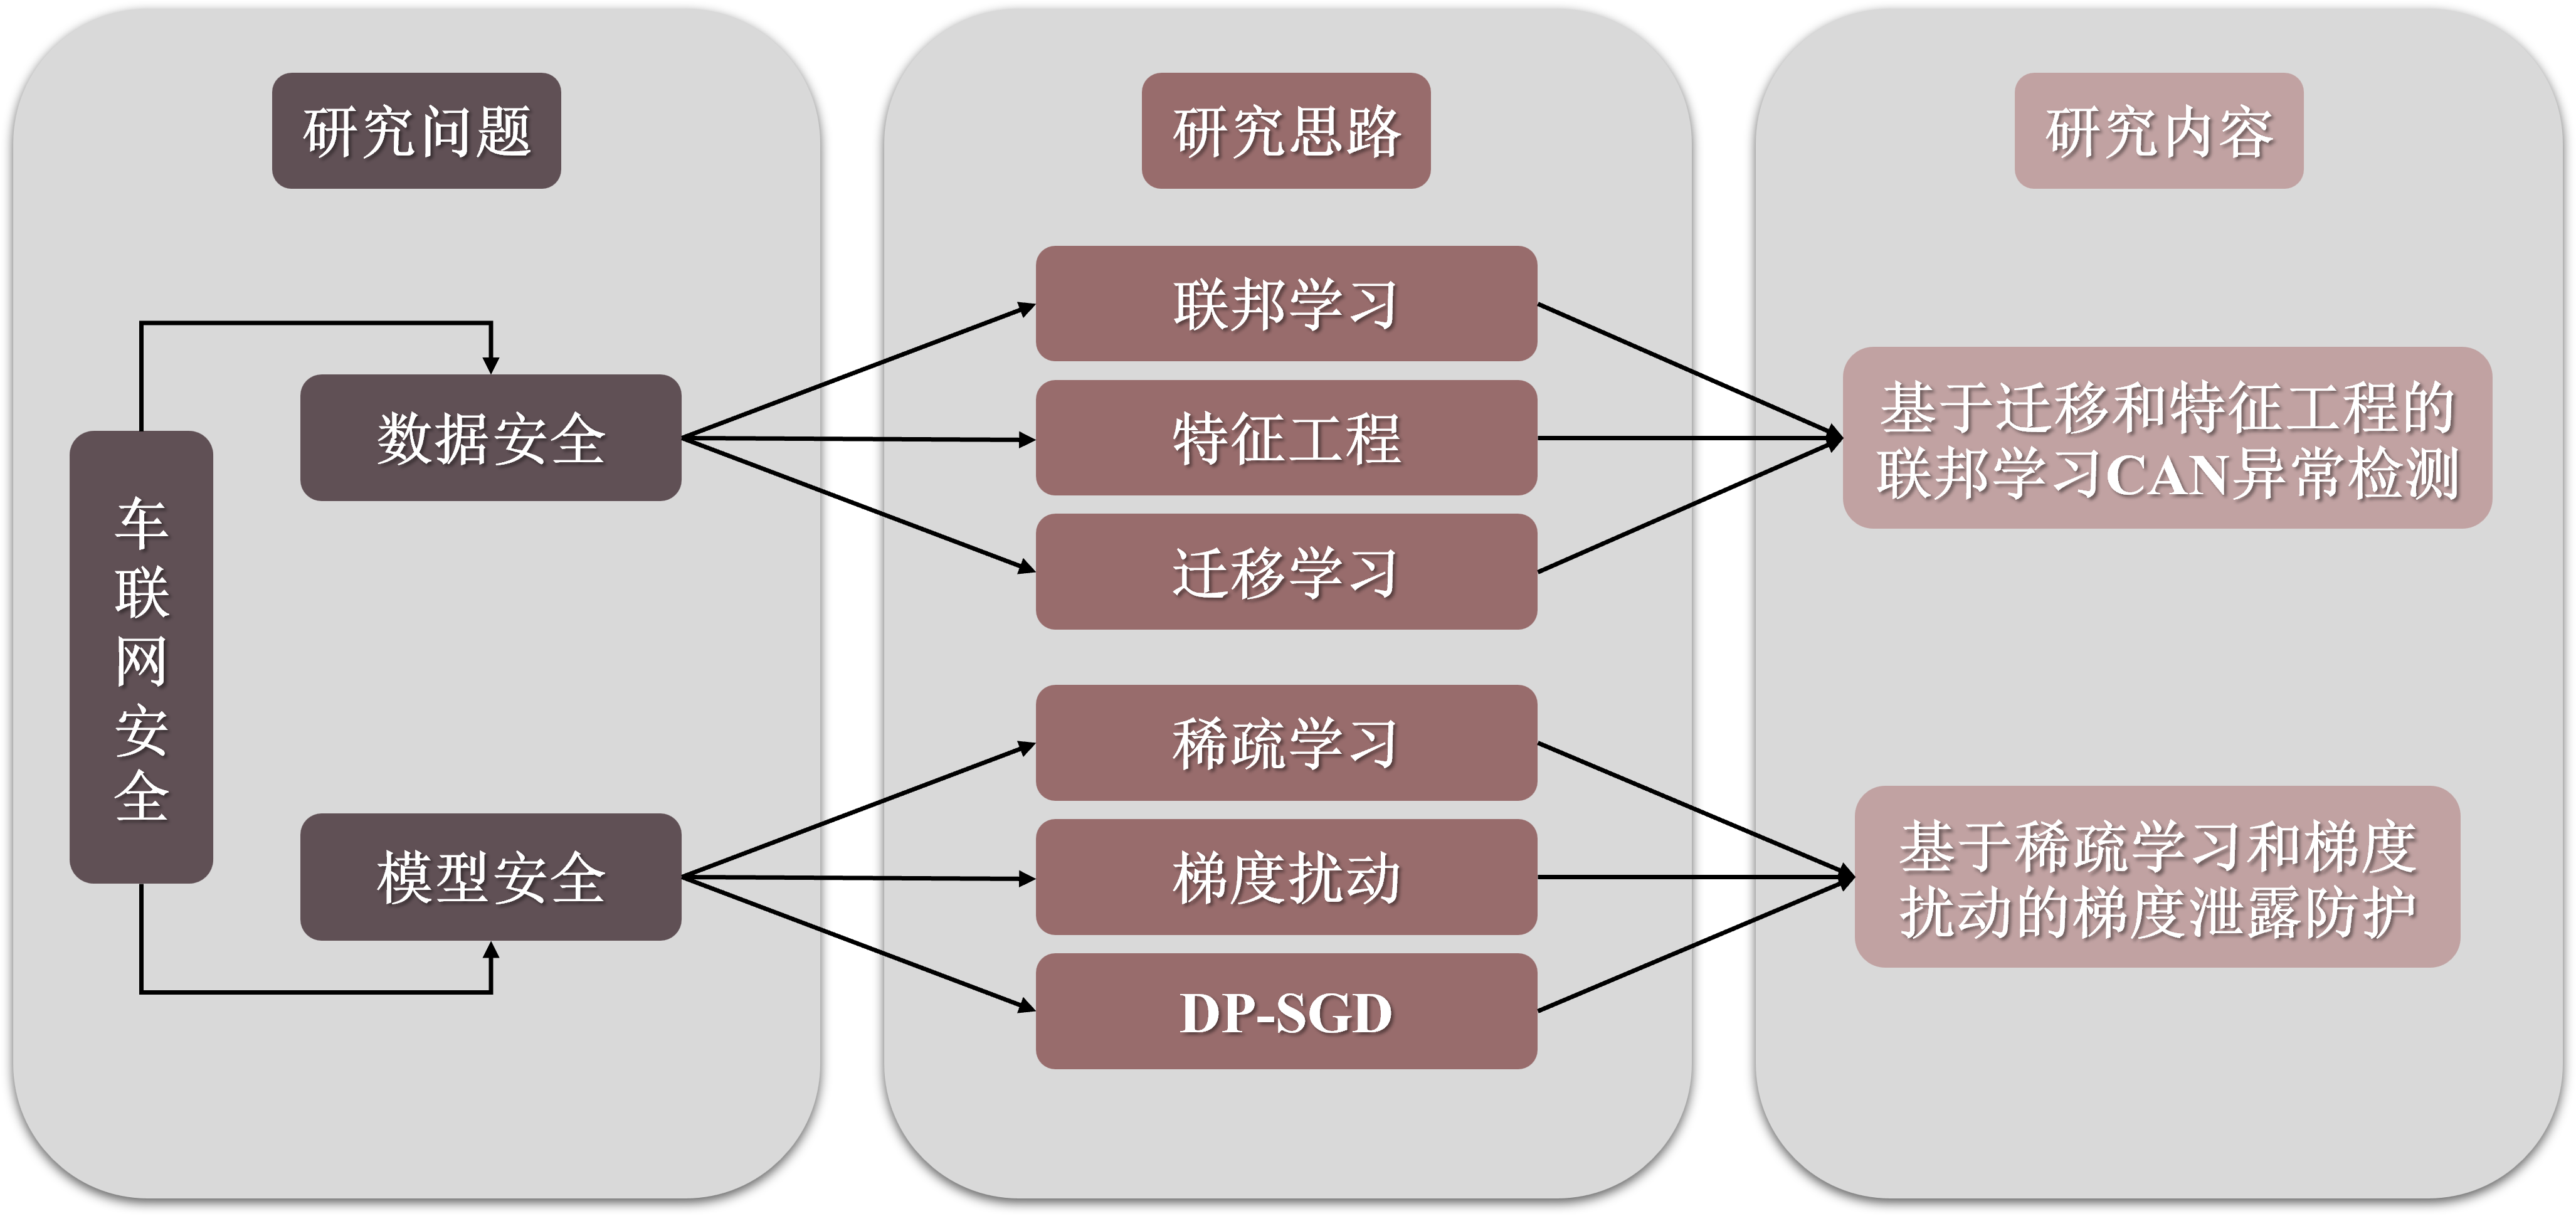
\includegraphics[width=1 \textwidth]{figures/chapter1/chapter1.2.png}
    \caption{基于联邦学习的车联网异常检测系统}
    \label{fig:Anomaly_detection_system_of_IoVFL}
\end{figure}

车联网利用IEEE802.11p协议构建了一个由车辆和路边基础设施组成的分布式网络,能够管理车辆及其相关网络产生的数据,并为交通管制、公共保护等各种服务提供数据支持\cite{ref5,Data_communication_in_VANETs}。本文将车联网中的攻击分为两类:一类是恶意的外部攻击,另一类是系统故障。恶意的外部攻击是指那些利用车辆或路边设备的漏洞,对车联网的功能和安全造成破坏的攻击。本文假设车辆的制造商以及RSU等相关设备的生产者是友善的,他们不会故意在制造过程中留有后门,因此,单个车辆和单个RSU都是友好而积极的参与者,车辆内部系统不存在恶意的破坏者。系统故障是指那些由于开发者的粗心或者其他原因,导致车辆或路边设备的软件或硬件出现异常的情况。一旦系统故障发生,系统中的参与者无法为其他参与者提供服务,在其他参与者眼中,其状态为离线。本文的第一个研究点是来自车辆内部的攻击,这类攻击会破坏系统功能,不仅危及驾驶者的安全,而且可能对公司财务和运营、乘客的隐私等方面造成影响\cite{ref6}。攻击者可以干扰智能车辆内部的通信,使其无法获取道路信息,例如利用BSM(Basic Safety Messages)发动的攻击\cite{Message_Sieving_to_Mitigate_Smart_Gridlock_Attacks_in_V2V},或者基于认知无线电(CR)的频谱感知数据伪造(SSDF)攻击和主用户仿真(PUE)攻击\cite{Defense_against_SSDF_Attack_and_PUE_Attack_in_CR-Internet_of_Vehicles_(IoVs)_for_Millimeter_Wave_Massive_MIMO_Beamforming_Systems}。由于车辆由多个组件构成,例如车辆机器、内部网关和控制器,它们的编译环境、操作系统和传输协议各不相同,现有的网络入侵检测系统无法完全预防和隔离针对车辆的威胁\cite{CANintelliIDS_Detecting_In-Vehicle_Intrusion_Attacks_on_a_Controller_Area_Network_Using_CNN_and_Attention-Based_GRU},例如破坏多传感器融合(MSF)算法的FusionRipper攻击\cite{Drift_with_Devil_Security_of_Multi-Sensor_Fusion_based_Localization_in_High-Level_Autonomous_Driving_under_GPS_Spoofing}。车内网络也容易受到攻击,黑客可以通过攻击CAN总线控制车辆主控制器,导致事故,例如针对CAN总线的攻击\cite{Cloaking_the_Clock_Emulating_Clock_Skew_in_Controller_Area_Networks,A_Survey_on_Controller_Area_Network_Reverse_Engineering,Implementation_of_a_bluetooth_attack_on_controller_area_network_CAN}。

本文对车内攻击的研究重点就是CAN总线。控制器局域网(CAN)总线是一个低容错的协议,主要用于ECU和车载汽车网络的实时通信\cite{Intrusion_Detection_System_CAN-Bus_In_Vehicle_Networks_Based_on_the_Statistical_Characteristics_of_Attacks},它具有低成本、抗噪和容错性高等特点,被广泛应用于车载网中。由于CAN发送的是实时性很高的报文,因此并不适合引入重安全机制。而入侵检测系统(IDSs)是一种预防性保护机制,可以在软件完整性验证\cite{ref9}之后作为第二道防线,实现持续性的事件监控\cite{ref10}。在车联网中使用IDSs可以非侵入性地运行,最小化对车联网的影响,同时IDSs可以与人工审计结合提醒安全人员注意潜在的威胁,以便他们能够更有效地保护客户的车辆免受威胁\cite{ref11}。然而,将传统入侵检测系统引入车联网领域将面临多种问题,首先是数据量爆炸问题,车联网中的节点可能在计算和内存方面受到限制。然而,深度学习模型的训练过程中,无论是数据采样还是分析,都将消耗大量的节点资源。因此,需要考虑模型对智能车带来的性能消耗问题。其次,车联网的动态性问题,车联网与物联网的一大区别就在于车辆的动态性,这意味着整个车联网的拓扑结构是频繁变化的,车辆节点接入网络具有随机性\cite{Attack_IOV2},这将导致不同地区的RSU所拥有的网络质量、收到的数据量等客观条件之间有较大的差异,然而,深度学习模型的检测性能与这些数值高度相关。这两个都可以归类为数据的非独立同分布问题。

车联网是一种利用车辆和路边基础设施之间的通信来提供智能交通服务的网络。车联网中的车辆可以收集和处理各种数据,例如位置、速度、方向、路况、天气、驾驶行为等,从而提高道路安全和效率,降低能耗和污染,增强驾驶体验和舒适度。为了实现这些目标,车联网中广泛使用了深度学习(DL)算法,例如卷积神经网络(CNN)、循环神经网络(RNN)、长短期记忆网络(LSTM)等,来处理图像、语音、文本、视频等多模态数据。然而,这些DL算法也带来了隐私和安全的挑战,因为它们可能会泄露训练数据的敏感信息。恶意的攻击者可以利用这些DL算法中泄露出来的梯度,通过一些逆向工程的技术,反推出原始数据,从而侵犯用户的隐私。例如,攻击者可以通过梯度重构攻击(GRA)\cite{Model_Inversion_Attacks_that_Exploit_Confidence_Information_and_Basic_Countermeasures},从梯度中恢复出图像或文本数据;或者通过成员推理攻击(MIA)\cite{Membership_Inference_Attacks_Against_Machine_Learning_Models},从梯度中判断某个数据是否属于训练集;或者通过属性推理攻击(AIA)\cite{Property_Inference_Attacks_on_Fully_Connected_Neural_Networks_using_Permutation_Invariant_Representations},从梯度中推断出某个数据的某个属性,例如性别、年龄、疾病等。这些攻击不仅威胁到用户的个人隐私,而且可能导致法律、道德、社会等方面的问题。因此,如何防御梯度泄露攻击,保护车联网中用户的隐私,是一个亟待解决的研究问题。

本文对DL模型攻击研究的重点是梯度泄露攻击(DLG),一种针对联邦学习系统的隐私攻击,它利用了参与者之间共享的梯度信息,来推测或重构出原始的训练数据。联邦学习是一种分布式机器学习的方法,它允许多个参与者在不共享数据的情况下,通过交换本地模型的更新来联合训练一个全局模型。这种方法被认为可以保护参与者的数据隐私,但是实际上,梯度中可能包含了训练数据的敏感信息,例如标签、属性、图像等。梯度泄露攻击的基本思想是,给定一个预训练的模型和一个共享的梯度,攻击者可以随机生成一对伪输入和标签,然后将其输入模型并计算伪梯度。接着,攻击者可以优化伪输入和标签,使得伪梯度和真实梯度之间的距离最小化。这样,伪输入和标签就会逐渐接近原始的训练数据。当优化过程完成后,攻击者就可以从伪输入和标签中获取私有的数据。这种攻击可以应用于不同的数据类型和模型结构,例如图像、文本、全连接层、卷积层等。梯度泄露攻击的危害范围很大,它可以影响中心化和去中心化的联邦学习系统。在中心化的系统中,参数服务器可以从每个参与者的梯度中窃取其本地训练数据。在去中心化的系统中,任何一个参与者都可以从与其交换梯度的其他参与者中窃取其训练数据。这些攻击不仅威胁到参与者的个人隐私,而且可能导致法律、道德、社会等方面的问题。梯度泄露攻击的防御方法有一些,例如梯度压缩、梯度噪声、差分隐私等。这些方法都有一定的效果,但也会带来一些性能损失或计算开销。

针对上述问题,本文所做的工作如下:

(1)为了解决车联网数据安全问题,本文提出了一种基于迁移和特征工程的联邦学习CAN异常检测。该系统采用联邦平均算法进行全局模型训练,只需在参与者之间交换本地模型的梯度,无需共享原始数据,从而节省了车联网的传输带宽。该系统还结合了迁移学习的思想,将CNN、VGG16、AlexNet、ResNet18等四种深度学习算法融合到联邦学习中,为用户提供了多种选择,同时减少了训练成本和数据需求。此外,针对车联网的动态性导致的数据异构问题,本文提出了一种针对CAN总线数据的特征工程方案,以提高分类模型的性能。最后,本文通过实验验证了所提出的模型的有效性。仿真结果显示,本文设计的框架能够显著提升车联网的安全性。

(2)为解决车联网中的模型安全问题,提出了一种基于稀疏学习和梯度扰动的梯度泄露防护方案。该方案的主要思想是,在RSU接收到训练数据之前,利用稀疏学习的方法,对原始数据进行系数学习和稀疏化处理,从而降低数据中的敏感信息泄露风险。在MEC进行全局模型训练时,从模型中提取表示层,根据表示层的$L_2$范数计算梯度筛,然后将梯度筛应用到表示层中,使得筛出来的部分梯度加上拉普拉斯噪声,从而扰乱表示层梯度中的信息。本文通过实验评估了所提出方案的有效性,结果表明,该方案能够有效地防止梯度泄露攻击,同时保持模型的性能。

\section{论文组织结构}

本文一共分为五章,具体内容如下: 

第一章\ 引言

本章主要介绍本文的研究背景、内容和框架。首先,从车联网目前面临的安全问题出发,分析了数据安全和模型安全在车联网应用场景中的重要性和挑战。其次,概述了本文的主要研究内容,包括车联网数据安全和模型安全的研究问题、方法和贡献。最后,说明了本文的组织结构和章节安排。

第二章\  研究现状

本章主要介绍车联网异常检测和梯度泄露的研究现状,分为两个部分:一是车联网数据安全的入侵检测系统(IDS)的发展现状,从基于普通深度学习算法的IDS、基于高级深度学习算法的IDS和关注于数据隐私保护的IDS三个角度进行分析;二是车联网模型安全的梯度泄露的发展现状,从基于优化的梯度泄露攻击和梯度泄露防御两个方面进行介绍。

第三章\  基于迁移和特征工程的联邦学习CAN异常检测

本章主要介绍了一种针对车联网安全中的数据安全问题而提出的有效方法,即基于迁移学习和特征工程的联邦学习CAN异常检测设计框架。首先,本章对相关工作和技术进行了简要的说明,其中涉及到了联邦学习、迁移学习和特征工程的技术原理。其次,本章对所提出的基于迁移和特征工程的联邦学习CAN异常检测框架进行了详细的阐述,包括了车辆与RSU之前的数据传输、RSU上的DL模型选择、MEC上的联邦学习等策略。最后,本章对说提出框架进行了实验测评和性能分析,验证了所提出框架的有效性和优越性。最后,本章对基于迁移和特征工程的联邦学习CAN异常检测的主要内容进行了总结和归纳。

第四章\  基于稀疏学习和梯度扰动的梯度泄露防护 

本章主要介绍了一种针对车联网安全中的模型安全问题而提出的有效的方法,即基于稀疏学习和梯度扰动的梯度泄露防护方法。首先,本章对相关的工作和技术进行了简要的说明,其中涉及到了特征提取与稀疏学习的相关概念和技术原理,以及差分隐私的相关概念和技术原理。其次,本章对所提出的基于稀疏学习和梯度扰动的梯度泄露防护方案进行了详细的阐述,包括了梯度泄露攻击模型的形式化定义、基于稀疏学习的数据隐私保护策略的具体实现和基于DP-SGD的梯度扰动策略的具体实现。最后,本章对所提出的方法进行了实验测评和性能分析,验证了所提出方法的有效性和优越性。最后,本章对基于稀疏学习和梯度扰动的梯度泄露防护方法的主要内容进行了总结和归纳。

第五章\  结论和未来工作 

本章总结了基于联邦学习的车联网异常检测系统的研究成果和展望。首先回顾了车联网数据安全和模型安全的问题及本文提出的解决方案,然后指出了本文的不足之处和改进方向,并提出了未来的研究计划。
 								%引言
 %      \setlength{\baselineskip}{20pt}
\chapter{研究现状}
\label{cha:chap2}

本章主要介绍基于联邦学习的车联网异常检测系统的研究现状,其中包括车联网异常检测,梯度泄露攻击、梯度泄露防御的相关研究以及目前存在的问题。

\section{车联网异常检测的研究现状}

\subsection{基于普通深度学习算法的IDS}

本节介绍了一些基于普通深度学习算法的车联网入侵检测系统,包括基于卷积神经网络(CNN)和基于卷积长短期记忆网络(ConvLSTM)的方法。这些方法主要利用了车联网中的链路负载数据和网络消息数据,来提取特征并进行分类或异常检测。这些方法的优点是能够有效地捕捉数据的时空特征,提高检测的准确性和鲁棒性。这些方法的缺点是没有考虑数据的隐私保护和模型的计算效率,可能存在泄露敏感信息或增加计算负担的风险。

Nie等人\cite{Date_Driven}提出了一种基于CNN的车联网入侵检测系统,该系统基于路边单元(RSU)的链路负载数据,来检测针对RSU的入侵行为。该系统使用了一个多层CNN架构,来提取链路负载数据的时空特征,并输出一个二分类结果,表示是否存在入侵。该系统还对CNN的收敛性进行了理论分析,证明了其在实际部署中的可行性。

Alladi等人\cite{ref13}提出了一种基于人工智能的车联网入侵检测架构,该架构部署在多接入边缘计算(MEC)服务器上,利用车辆流量数据,来检测车联网中的异常事件。该架构提出了两种基于CNN的分类技术,一种是直接基于时间序列的分类,另一种是基于序列图像的分类。两种技术都将车辆流量数据转换为一维或二维的输入,然后通过CNN进行特征提取和分类。实验结果表明,基于序列图像的分类技术表现最佳。该架构的优点是具有成本效益,因为可以利用现有的MEC服务器,无需额外的基础设施投资。Alladi等人\cite{ref14}在\cite{ref13}的基础上,进一步探索了不同的深度学习模型在车联网入侵检测中的表现,包括CNN、循环神经网络(RNN)、长短期记忆网络(LSTM)和门控循环单元(GRU)。他们设计了三种不同的分类方案,分别是单阶段粗粒度分类、单阶段细粒度分类和两阶段分类。实验结果表明,单阶段细粒度分类方案在所有模型中表现最佳,两阶段分类方案也有相当的性能。他们还提出了一种基于应用场景和数据可用性的模型选择方法,可以根据不同的需求,选择最合适的模型进行部署。

Yang等人\cite{Federated-AI-Enabled-IDS}提出了一种基于ConvLSTM的车联网入侵检测方法,该方法利用了车联网中的网络消息数据,来检测针对智能车辆(ICV)的入侵行为。该方法使用了一个ConvLSTM模型,来提取网络消息数据的时空特征,并输出一个多分类结果,表示不同类型的入侵。为了训练ConvLSTM模型,该方法采用了一种联合学习(FL)框架,其中ICV作为本地客户端,MEC服务器作为参数服务器。该方法还开发了一种基于近端策略优化(PPO)的联邦客户端选择(FCS)方案,来优化FL框架的性能,提高训练的效率和隐私保护。

\subsection{基于高级深度学习算法的IDS}

本节介绍了一些基于高级深度学习算法的车联网入侵检测系统,包括基于LSTM和GRU的混合模型、基于树模型的集成方法、基于CNN的迁移学习和集成学习方法、基于Transformer的变体模型和基于BERT的预训练模型。这些方法主要利用了车联网中的网络消息数据和车辆流量数据,来提取特征并进行分类或异常检测。这些方法的优点是能够有效地处理高维、非线性、时序的数据,提高检测的准确性和鲁棒性。这些方法的缺点是没有考虑数据的隐私保护和模型的计算效率,可能存在泄露敏感信息或增加计算负担的风险。

Ullah等人\cite{ref15}提出了一种基于LSTM和GRU的混合深度学习模型,用于车联网入侵检测。该模型结合了LSTM和GRU的优势,能够捕捉数据的长期和短期依赖性,并减少训练和响应时间。Yang等人\cite{ref16}提出了一种基于树模型的智能入侵检测系统,适用于自动驾驶汽车的CAN总线和普通车联网。该系统使用了决策树、随机森林、额外树和XGBoost等树模型,能够处理高维、非线性的数据,并提高检测的速度和效果。之后,Yang等人\cite{A_Transfer_Learning_and_Optimized_CNN_Based_Intrusion_Detection_System_for_Internet_of_Vehicles}又提出基于CNN和超参数优化技术,提出了一种基于迁移学习和集成学习的车联网入侵检测系统。该系统利用了迁移学习的思想,将预训练的CNN模型迁移到车联网的数据上,并使用超参数优化技术来调整模型的参数。该系统还使用了集成学习的方法,将多个CNN模型的输出进行融合,以提高检测的稳定性和准确性。实验结果表明,该系统的检测率和f1值均超过99.25\%。同时,Yang等人\cite{ref18}还提出了一种新的集成IDS框架LCCDE,用于检测各种类型的网络攻击。该框架选择了XGBoost、LightGBM和CatBoost这三种表现最好的机器学习模型,构建了一个多分类器。该框架还利用了类领袖模型的预测置信度,来做出准确的决策,以提高检测的可靠性和效率。

Wu等人\cite{RTIDS}提出了一种具有鲁棒性的基于Transformer的入侵检测系统RTIDS。该系统使用了一个变体的堆栈编码器-解码器神经网络,从高维原始数据中学习低维特征表示。该系统还利用了自注意力机制,来促进网络流量类型的分类,以提高检测的灵敏度和精确度。Alkhatib等人\cite{can_ids}提出了一种名为CAN-BERT的基于深度学习的网络入侵检测系统,用于检测对CAN总线协议的网络攻击,提高CAN总线协议的安全性。该系统使用了一个预训练的BERT模型,来提取CAN消息数据的语义特征,并输出一个二分类结果,表示是否存在入侵。该系统的优点是能够实时地检测网络攻击,减少延迟和误报。

\subsection{基于于数据隐私保护的IDS}

本节介绍了一些关注于数据隐私保护的车联网入侵检测系统,包括基于联邦学习和拉格朗日编码的方法。这些方法主要利用了车联网中的CAN数据和流量数据,来检测智能网联汽车的网络入侵。这些方法的优点是能够在保护数据隐私的同时,提高检测的准确性和安全性。这些方法的缺点是需要额外的计算资源和通信开销,可能影响检测的效率和实时性。

Yu等人\cite{Federated-LSTM}提出了一种基于联邦学习的LSTM模型,用于检测智能网联汽车的网络入侵。该模型基于车联网系统模型和CAN数据框架,利用车辆之间的协作学习,来提取CAN数据的时序特征,并输出一个二分类结果,表示是否存在入侵。该模型通过仿真实验,验证了其对各种类型的攻击的检测精度超过90%。

Hbaieb等人\cite{Federated_Learning_Based_IDS_Approach_for_the_IoV}提出了一种基于联邦学习的入侵检测系统,旨在为车联网提供安全解决方案。该系统部署在软件定义网络的结构下,利用车辆的流量数据,来检测车联网中的异常事件。该系统集成了信任指标,以帮助保护车联网的安全。该系统还利用车辆的数据包丢弃率和节点身份,来进行协作学习,提高检测的效果。

Ni等人\cite{Lagrange_Coded_Federated_Learning}提出了一种新方法,用于提高车联网系统中联邦学习的准确性和安全性。该方法基于拉格朗日编码计算的概念,为车辆处理的数据引入了计算冗余,以抵抗潜在的攻击和故障。该方法设计了一个名为L-CofL的拉格朗日编码的FL模型,支持将LCC与FL集成,以实现安全的车联网系统。该方法通过理论分析和实验评估,证明了其在准确性和安全性方面的优势。

\section{梯度泄露攻击的研究现状}
\subsection{基于优化的梯度泄露攻击研究现状}

随着深度神经网络的广泛应用,分布式学习系统(如协同学习、联邦学习等)也越来越受到关注。这些系统通过在多个客户端之间交换梯度信息,实现了在不共享原始数据的情况下协同训练一个神经网络。然而,近年来的研究表明,梯度信息可能会泄露客户端的私有数据,从而威胁到用户的隐私安全。

Hitaj等人\cite{Deep_Models_Under_the_GAN}是基于优化方法的先驱,他们在2017年提出了生成对抗网络泄露攻击DMU-GAN,利用生成对抗网络(GAN)从梯度中重建出训练集中的数据分布。他们的方法可以处理多个输入点的情况,但需要访问一个与训练集相似的辅助数据集。并且,尽管DMU-GAN可以生成类似于私有数据集的数据,但它无法提取单个数据点。在2019年,Zhu等人\cite{DLG}提出了深度梯度泄露(Deep Leakage from Gradients,DLG),首次展示了从公开共享的梯度中恢复出私有训练数据的可能性。他们的方法利用梯度匹配的思想,通过优化一个虚拟数据和对应的标签,使其与真实数据产生的梯度尽可能相似。他们的方法不需要知道输入的类别标签,也不需要任何辅助数据集,且适用于任何可微分的模型和损失函数。他们在计算机视觉和自然语言处理的任务上验证了其有效性,表明其攻击能够实现像素级的精确重建和词汇级的匹配。然而,DLG的方法也存在一些局限性,如收敛困难、标签发现不稳定、对梯度压缩不敏感等。为了克服DLG的局限性,一些改进的方法被提出。Zhao等人\cite{iDLGID}在2020年提出了改进的深度梯度泄露(Improved Deep Leakage from Gradients,iDLG),针对梯度压缩的情况,重新设计了优化目标函数,使得压缩后的虚拟梯度与压缩后的真实梯度相似。他们还设计了一种新的虚拟数据初始化方法,以补偿梯度压缩造成的信息损失。他们的方法可以从高度压缩的梯度(0.1\%压缩率)中恢复出准确的数据和标签,而DLG的方法只能支持70\%的压缩率,从而实现了700倍的改进。

在梯度反演的攻击方法方面。Yin等人\cite{DeepInversion}在2020年提出深度反演(DeepInversion),利用梯度优化的方法,从随机噪声中生成自然图像,同时匹配梯度、图像先验和块间的总变分正则化。此外,使用自适应深度反演,通过最大化教师和学生网络对数之间的Jensen-Shannon散度,来提高合成图像的多样性。他们在CIFAR-10和ImageNet数据集上训练的网络的合成图像显示出高保真度和真实感,并帮助实现了一种新的无数据应用——不需要任何真实图像或标注数据的应用。在这之后第二年,Yin等人\cite{GradInversion}提出梯度反演(GradInversion),针对视觉变换器(Vision Transformer,ViT)的情况,利用梯度优化的方法,从随机噪声中生成自然图像,同时匹配梯度、图像先验和块间的总变分正则化。他们的方法在ImageNet1K和MS-Celeb-1M数据集上展示了高保真度和真实性的图像重建,且发现视觉变换器比之前研究的卷积神经网络更容易受到梯度反演攻击的影响。另一种新颖的方法是,Hatamizadeh等人\cite{GradViT}在2022年提出的GradViT,针对大批量数据的情况,利用梯度无关的优化方法(如进化策略和贝叶斯优化),从梯度中重建出高质量的图像。他们的方法在复杂的数据集、深层的网络和大批量的情况下,都能实现与原始数据的高保真度和接近度,且提出了一种用于衡量梯度泄露量的实证工具。

在真实的FL场景中,原始全梯度的直接传输非常消耗资源,因此参与者更希望在将局部梯度发送回服务器之前压缩局部梯度,以减少通信开销\cite{Gradient_Leakage_Attacks_in_Federated_Learning}。针对梯度压缩的情况,一种有效的数据重建攻击是Yang等人\cite{HCGLA}在2023年提出来的HCGLA,它针对DLG的不合理的优化目标函数,重新设计了一个合理的目标函数,使得压缩后的虚拟梯度与压缩后的真实梯度相似。该方法还设计了一种新的虚拟数据初始化方法,以补偿梯度压缩造成的信息损失。该方法可以从高度压缩的梯度(0.1\%压缩率)中恢复出准确的数据和标签,而DLG的方法只能支持70\%的压缩率,从而实现了700倍的改进。

针对联邦学习的情况,Geiping等人\cite{Inverting_Gradients}基于iDLG,在2020年提出了一种从梯度中恢复输入数据的数值重构方法IG,将梯度泄露攻击带入联邦学习领域。他们利用一个幅度不变的损失函数,来解决梯度操作的非线性问题。他们还证明了任何输入到一个全连接层的数据都可以解析地重构,而与剩余的网络结构无关。他们的方法在真实的深度和非光滑的网络上展示了从梯度中重构输入数据的可能性,即使在多个迭代或多张图像上进行梯度平均的情况下。一种新的隐私泄露方式是Li等热\cite{GGL}在2022年提出来的GGL,利用从公共图像数据集中学习的GAN的潜在空间作为先验,来补偿梯度降级过程中造成的信息损失。该方法还探索了各种无梯度优化方法,如进化策略和贝叶斯优化,来提高梯度反演的效果。该方法希望作为一种工具,用于实证地测量隐私泄露的量,从而促进更强大的防御机制的设计。

综上所述,梯度反演的问题是深度学习中的一个重要的安全挑战,它涉及到多个方面的研究,如攻击方法、防御方法、模型结构、应用场景等。这些研究对于理解和保护深度学习中的隐私具有重要的意义和价值。然而,目前的研究还存在一些不足和局限,如梯度反演的理论分析、梯度反演的评估标准、梯度反演的通用方法等。因此,梯度反演的问题还需要进一步的探索和深入的研究。

\section{梯度泄露防御的研究现状}

联邦学习能保护用户隐私和数据安全。但是这里不可避免地又带来了联邦学习自身的数据泄露风险,正如Yang等人\cite{Gradient_Leakage_Attacks_in_Federated_Learning}提到需要进一步研究 GLA 防御策略。目前,两种主要的防御方法包括向梯度添加高斯噪声和实施基于密码的方法。然而,前者是以模型准确性为代价的,找到平衡点仍然具有挑战性。后者不仅需要修改模型结构,而且在更新全局模型时会消耗大量的带宽和存储资源。针对梯度泄露的防御方法,主要有以下几种:(1)在共享梯度之前添加噪声,如差分隐私、同态加密等,但这些方法\cite{Efficient_Privacy-Preserving_Federated_Learning_Against_Inference_Attacks_for_IoT,Mixed_Quantization_Enabled_Federated_Learning_To_Tackle_Gradient_Inversion_Attacks,Revealing_and_Protecting_Labels_in_Distributed_Training,FedML-HE_An_Efficient_Homomorphic-Encryption-Based_Privacy-Preserving_Federated_Learning_System,Distributed_Learning_in_Trusted_Execution_Environment_A_Case_Study_of_Federated_Learning_in_SGX}会降低梯度的有效性,影响模型的训练效果;(2)使用梯度压缩,如量化、稀疏化、低秩近似等,但这些方法并不能完全阻止梯度泄露,只能提高攻击的难度;(3)使用梯度掩码,如梯度修剪、梯度过滤等,但这些方法可能会损失梯度的重要信息,导致模型的性能下降;(4)使用梯度混淆,如梯度扰动、梯度混合等,但这些方法可能会引入额外的计算开销,且需要设计合适的混淆策略。

\subsection{基于梯度变换的梯度防御方案}

基于梯度变换的主要思想是在联邦学习中对梯度进行一定的变换,以降低梯度泄露的风险。变换的方式包括压缩、量化、稀疏化、扰动等。这类方法的优点是可以有效地减少梯度的信息量,从而提高隐私保护的水平。缺点是变换可能会影响梯度的质量,从而降低模型的性能。此外,一些变换也可能引入额外的计算或通信开销。一些研究\cite{An_Optimized_Sparse_Response_Mechanism_for_Differentially_Private_Federated_Learning,PrivateDL_Privacy-preserving_collaborative_deep_learning_against_leakage_from_gradient_sharing}使用基于梯度稀疏化和差分隐私的防御方法,使得保持模型性能的同时,提供可量化的隐私保证。而另一些\cite{Gradient-Leakage_Resilient_Federated_Learning,DataLens_Scalable_Privacy_Preserving_Training_via_Gradient_Compression_and_Aggregation}则采用基于梯度压缩和聚合的防御方法,在保持模型性能的同时,实现可扩展的梯度隐私保护,并保证模型的收敛性和准确性。梯度稀疏化是指只选择部分重要的梯度进行传输或更新,从而减少梯度的维度和通信开销而差分隐私是指在梯度上添加随机噪声,从而保证梯度的统计特性不会泄露单个样本的信息。这两种方法的结合可以提高模型的隐私保护水平,但也会带来一定的性能损失。梯度量化是指将连续的梯度值映射到离散的集合中,从而减少梯度的位数和存储空间而随机化是指在梯度上引入一定的随机性,从而减少梯度的冗余和相关性。这两种方法的结合可以提高模型的训练效率和通信效率,但也会带来一定的精度损失。总的来说,梯度稀疏化和差分隐私的防御方法主要关注模型的隐私安全性,而梯度量化和随机化的防御方法主要关注模型的训练速度。Jing Wu等人\cite{Concealing_Sensitive_Samples_against_Gradient_Leakage_in_Federated_Learning}认为模型反演攻击主要利用了梯度信息中包含的数据信息,因此提出了DCS2——一种通过生成隐蔽样本来混淆敏感数据梯度的方法。隐蔽样本是指在梯度层面与敏感数据相似,但在视觉层面与敏感数据不同的样本,这样可以使得攻击者无法从梯度中重建敏感数据,同时又不影响联邦学习的性能。隐蔽样本地生成使用余弦相似度进行衡量,最大化隐蔽样本和敏感样本之间的不相似性,而使用GEM技术进行梯度投影和改进mixup正则以保证加入的隐藏样本与原始小批量梯度对齐,以便服务器能够有效地更新模型参数。Chen等人\cite{QP-LDP_for_better_global_model_performance_in_federated_learning}提出的QP-LDP算法一种基于梯度量化和局部差分隐私的防御方法,可以在提供隐私保证的同时,改善全局模型的性能。具体的来说,作者将整个算法分为了三个部分,梯度量化部分采用了一种基于聚类的量化方法,将梯度向量划分为若干个子向量,然后对每个子向量进行聚类,得到聚类中心和聚类标签。聚类中心表示了梯度的主要方向,聚类标签表示了梯度的细节信息。作者只需要共享聚类中心和聚类标签,而不需要共享原始的梯度向量,从而实现了梯度的压缩。为了增加梯度的不确定性,提高隐私保护的水平,在第二部分中采用一种基于拉普拉斯噪声的扰动方法,将噪声添加到聚类中心和聚类标签上。最后采用了一种基于加权平均的聚合方法,将来自不同客户端的量化和扰动后的梯度进行聚合,得到全局模型的更新梯度。

\subsection{基于梯度修剪的梯度防御方案}

基于梯度修剪的防御方法的主要思想是在联邦学习中对梯度进行修剪,以降低梯度泄露的风险。修剪的方式包括剪枝、对齐、过滤等。这类方法的优点是可以有效地减少梯度的敏感度,从而提高隐私保护的水平。缺点是修剪可能会影响梯度的有效性,从而降低模型的性能。此外,一些修剪也可能引入额外的计算或通信开销。PriPrune\cite{PriPrune_Quantifying_and_Preserving_Privacy_in_Pruned_Federated_Learning}是一种结合了梯度剪枝和量化的防御方法,旨在提高用户数据的隐私保护。它的基本思想是:在每轮联合学习中,用户设备先对自己的本地模型进行修剪,去除一些不重要的参数或连接;然后,用户设备对修剪后的模型进行量化,即将参数的值映射到一些离散的数值,从而进一步降低模型的精度和敏感性; 最后,用户设备将量化后的模型上传到服务器,服务器对不同用户的模型进行聚合,得到一个全局的模型,并将其发送回用户设备。它的不足之处在于需要用户设备具备一定的计算能力和存储空间,因为修剪和量化都需要在用户设备上进行,而且需要保存修剪和量化的信息。并且还需要服务器和用户设备之间有一定的信任度,因为服务器需要知道用户设备的修剪和量化的参数和方法,以便正确地聚合模型,而用户设备需要信任服务器不会滥用或泄露自己的模型。Zhiqiu Z等人\cite{Preserving_data_privacy_in_federated_learning_through_large_gradient_pruning}提出了一种基于梯度大幅剪枝的防御方法,可以在保护数据隐私的同时,提高联邦学习的效率。具体来说,作者提出了两种防御机制,分别是:(1)严格的大梯度剪枝(SLGP):这种机制将每一层的梯度按绝对值大小降序排序,并将大于一个阈值的梯度剪枝为零。这样可以减少梯度中包含的私有数据信息,从而防止对手利用梯度匹配的方法来重建数据。阈值的选择可以根据一些指标,如PSNR,来自动调整,以满足隐私保护的要求。(2)宽松的大梯度剪枝(RLGP):这种机制不是直接将大梯度剪枝为零,而是根据每一层梯度的$l_2$范数值来对大梯度进行不同程度的剪枝。如果$l_2$范数值大于1,那么大梯度会被该值除以,从而缩小其大小;如果$l_2$范数值小于等于1,那么大梯度仍然会被剪枝为零。这样可以避免对一些参数较少的模型造成不稳定的训练过程。这篇论文的防御方法需要选择合适的剪枝阈值,但是这个阈值可能会影响模型的效果和隐私保护的程度,而且这个阈值可能需要根据不同的数据集和模型来调整,没有给出一个通用的方法。Jiahui H等人\cite{Shield_Against_Gradient_Leakage_Attacks_Adaptive_Privacy-Preserving_Federated_Learning}提出的AdpPPFL框架可为联邦学习提供自适应的隐私保护功能。具体的来说,在每一轮通信$t$中,1)服务器运行泄露风险感知的隐私分解机制,获取分配给本轮的隐私预算$ϵ_t$以及分配给$K$个随机选择的客户端的隐私预算$\{\epsilon_{t}^{i}\}_{i=1}^{K}$;2)服务器向客户端广播全局模型$w^{t-1}$和$\{\epsilon_{i}^{i}\}_{i=1}^{K}$;3)每个客户端$i$采用自适应隐私保护的本地训练机制进行本地模型训练,然后将生成的模型更新$w^t_i$上传到服务器进行聚合。

\subsection{基于梯度扰动的梯度防御方案}

基于梯度扰动的防御方法的主要思想是在联邦学习中对梯度进行扰动,以降低梯度泄露的风险。扰动的方式包括加噪、旋转、变换等。这类方法的优点是可以有效地增加梯度的不确定性,从而提高隐私保护的水平。缺点是扰动可能会影响梯度的方向,从而降低模型的性能。此外,一些扰动也可能引入额外的计算或通信开销。例如,Soteria\cite{Soteria}是一种联邦学习中的隐私防御方法,它通过在神经网络的某一层添加扰动,降低数据的可重构性,同时保持模型的训练效果。设 $H$ 是一个有 $L$ 层的神经网络,每层的大小为 $n_1,\ldots,n_L$,输入层的大小为 $n_0$。令 $X$ 和 $X^{\prime}\in\mathbb{R}^{n_0}$ 分别表示 $H$ 的原始输入和重建输入, $h_{i,j}: \mathbb{R} ^{n_i}\to \mathbb{R} ^{n_j}$ 表示 $H$ 的第 $i$ 层到第 $j$ 层之间的映射函数。对于选定的防御层 $l$,用 $r= h_{0, l- 1}( X) $ 和 $r^{\prime}= h_{0, l- 1}( X^{\prime})$ 分别表示 $X$ 和 $X^{\prime}$ 在该层的中间表示,并求解以下优化问题:$\max_{r'}||X-X'||_2\text{ s.t. }||r-r'||_0\leq\epsilon.$。该问题的目标是找到一个最小的扰动 $r^{\prime}-r$,使得重建输入 $X^{\prime}$ 与原始输入 $X$ 的差异最大。由于攻击者无法直接观察到 $r$ 和 $r^{\prime}$,这相当于在防御层 $l$ 上生成了一个扰动的梯度。因此,Soteria 的客户端不再发送原始的梯度 $\nabla W$,而是发送扰动的梯度 $\nabla W^{\prime}$,其中 $\nabla W_l^{\prime}$ 是根据扰动的中间表示 $r^{\prime}$ 计算的。PGL\cite{Protect_Privacy_from_Gradient_Leakage_Attack_in_Federated_Learning}也是一种在本地客户端进行随机梯度扰动的方案,不同与上者,PGL直接在梯度上进行的扰动而不是只扰动表示层,使用梯度相对于输入的雅可比矩阵来反映隐私泄露风险。Yongqi J等人\cite{Directional_Privacy_for_Deep_Learning}提出了一种新颖的隐私保护联邦学习方法,它采用了双重扰动的策略。首先,它在条件生成对抗网络(CGAN)的目标函数中加入了一个特征提取器和一个模糊函数,以提高生成数据的质量和多样性。然后,它将生成数据和真实数据混合,形成虚假的训练数据,用于更新中心模型,从而减少真实数据的泄露风险。其次,它对全连接层的梯度进行了扰动,方法是用一个与梯度维度相同的矩阵进行 Hadamard 乘积。这个矩阵是根据一个目标函数生成的,该目标函数旨在使得推断出的特征表示尽可能接近真实特征表示,而重建出的数据尽可能远离真实数据。通过这种方法,它可以有效地抵抗推断攻击,同时保持较高的准确率。更多的扰动方案还有,Fei W等人\cite{More_than_Enough_is_Too_Much_Adaptive_Defenses_against_Gradient_Leakage_in_Production_Federated_Learning}提出来的Outpost、Xue Y等人\cite{An_Accuracy-Lossless_Perturbation_Method_for_Defending_Privacy_Attacks_in_Federated_Learning} 提出的联邦学习模型扰动方法。

\subsection{基于数据变换的梯度防御方案}

基于数据变换的防御方法的核心思想是在联邦学习的过程中对数据进行不同形式的变换,从而减少梯度泄露的可能性。这些变换包括对数据进行分解、转换、扩展等操作。这种方法的优势在于能够有效地提升数据的多样性,进而增强隐私保护的效果。然而,这种方法也存在一些局限性,例如变换可能会损害数据的质量,导致模型的性能下降。另外,一些变换还可能增加计算或通信的成本。例如,Wei G等人\cite{Automatic_Transformation_Search_Against_Deep_Leakage_From_Gradients}提出了一种名为ATS的方案,它利用随机搜索的方法从数据增强库中选择最佳的变换策略。Jing L等人\cite{Safeguard_the_Original_Data_in_Federated_Learning_via_Data_Decomposition}则使用稀疏字典学习(DL)或QR分解的技术对原始数据进行隐私保护的处理。PRECODE\cite{PRECODE_A_Generic_Model_Extension_to_Prevent_Deep_Gradient_Leakage}采用变分建模的方式,在模型的某一层添加一个随机采样的瓶颈层,从而有效地阻断梯度泄露的途径。Yuting M等人\cite{Privacy-preserving_Collaborative_Learning_with_Scalable_Image_Transformation_and_Autoencoder}设计了一种基于图像变换和自编码器的隐私保护协同学习方案,它能够在多个数据源之间共享一个预测任务,同时提升机器学习模型的性能,防止敏感数据被梯度重构攻击泄露。该方案通过调节块大小,对训练图像进行随机排列,破坏图像的空间结构和语义信息。自编码器则用于从变换后的图像中学习有用的特征表示,以适应高维图像的分类任务。

综上所述,梯度泄露是一个严重的隐私威胁,需要引起人们的高度重视。目前的研究还存在一些不足,如攻击方法的通用性、防御方法的有效性、梯度泄露的理论分析等,需要进一步的探索和完善。

\section{本章小结}

本章介绍了车联网异常检测和梯度泄露的研究现状,分为两个部分。首先介绍了车联网数据安全的入侵检测系统(IDS)的发展现状,从基于普通深度学习算法的IDS、基于高级深度学习算法的IDS和关注于数据隐私保护的IDS三个角度进行分析。其次,介绍了车联网模型安全的梯度泄露的发展现状,在攻击方面介绍了基于优化的梯度泄露攻击,而防御方面介绍了基于梯度变换的梯度防御策略、基于梯度修剪的梯度防御方案、基于梯度扰动的梯度防御方案和基于数据变换的梯度防御方案4个方面。最后,本章指出了目前的研究存在的一些不足和局限,如梯度反演的理论分析、梯度反演的评估标准、梯度反演的通用方法等,需要进一步的探索和完善。 								%第二章
	% \setlength{\baselineskip}{20pt}
\chapter{基于迁移和特征工程的联邦学习CAN异常检测}
\label{cha:chap3}

\section{相关工作和技术介绍}

\subsection{联邦迁移学习}
联邦学习是保护输入隐私的分布式计算范式,可以实现各个客户端数据不共享的条件下的协同计算。具体来说,服务器与各个客户端通过中间结果的多轮交互来获得计算结果,在整个计算过程中,客户端的数据始终存储在本地,同时其他客户端和服务器对该客户端的数据没有任何访问权限。在客户端知情并且同意隐私政策的前提下,联邦学习满足数据最小化原则。在每轮迭代过程中,客户端仅为特定的计算任务传输必要的更新,同时,服务器仅短暂存储中间结果以即时完成聚合,并仅发布最终的计算结果。然而,现有工作表明,攻击者可以依据中间结果获得原始数据的一些信息,因此,联邦学习还需结合安全多方计算或同态加密等来增强计算过程的保密性,并结合差分隐私来增强结果发布的匿名性。目前,谷歌、微众银行、达摩院及百度等机构发布了联邦学习开源框架,并且联邦学习已经在政务、金融和医疗等场景中得到应用。

\begin{figure}[htb]
\centering
    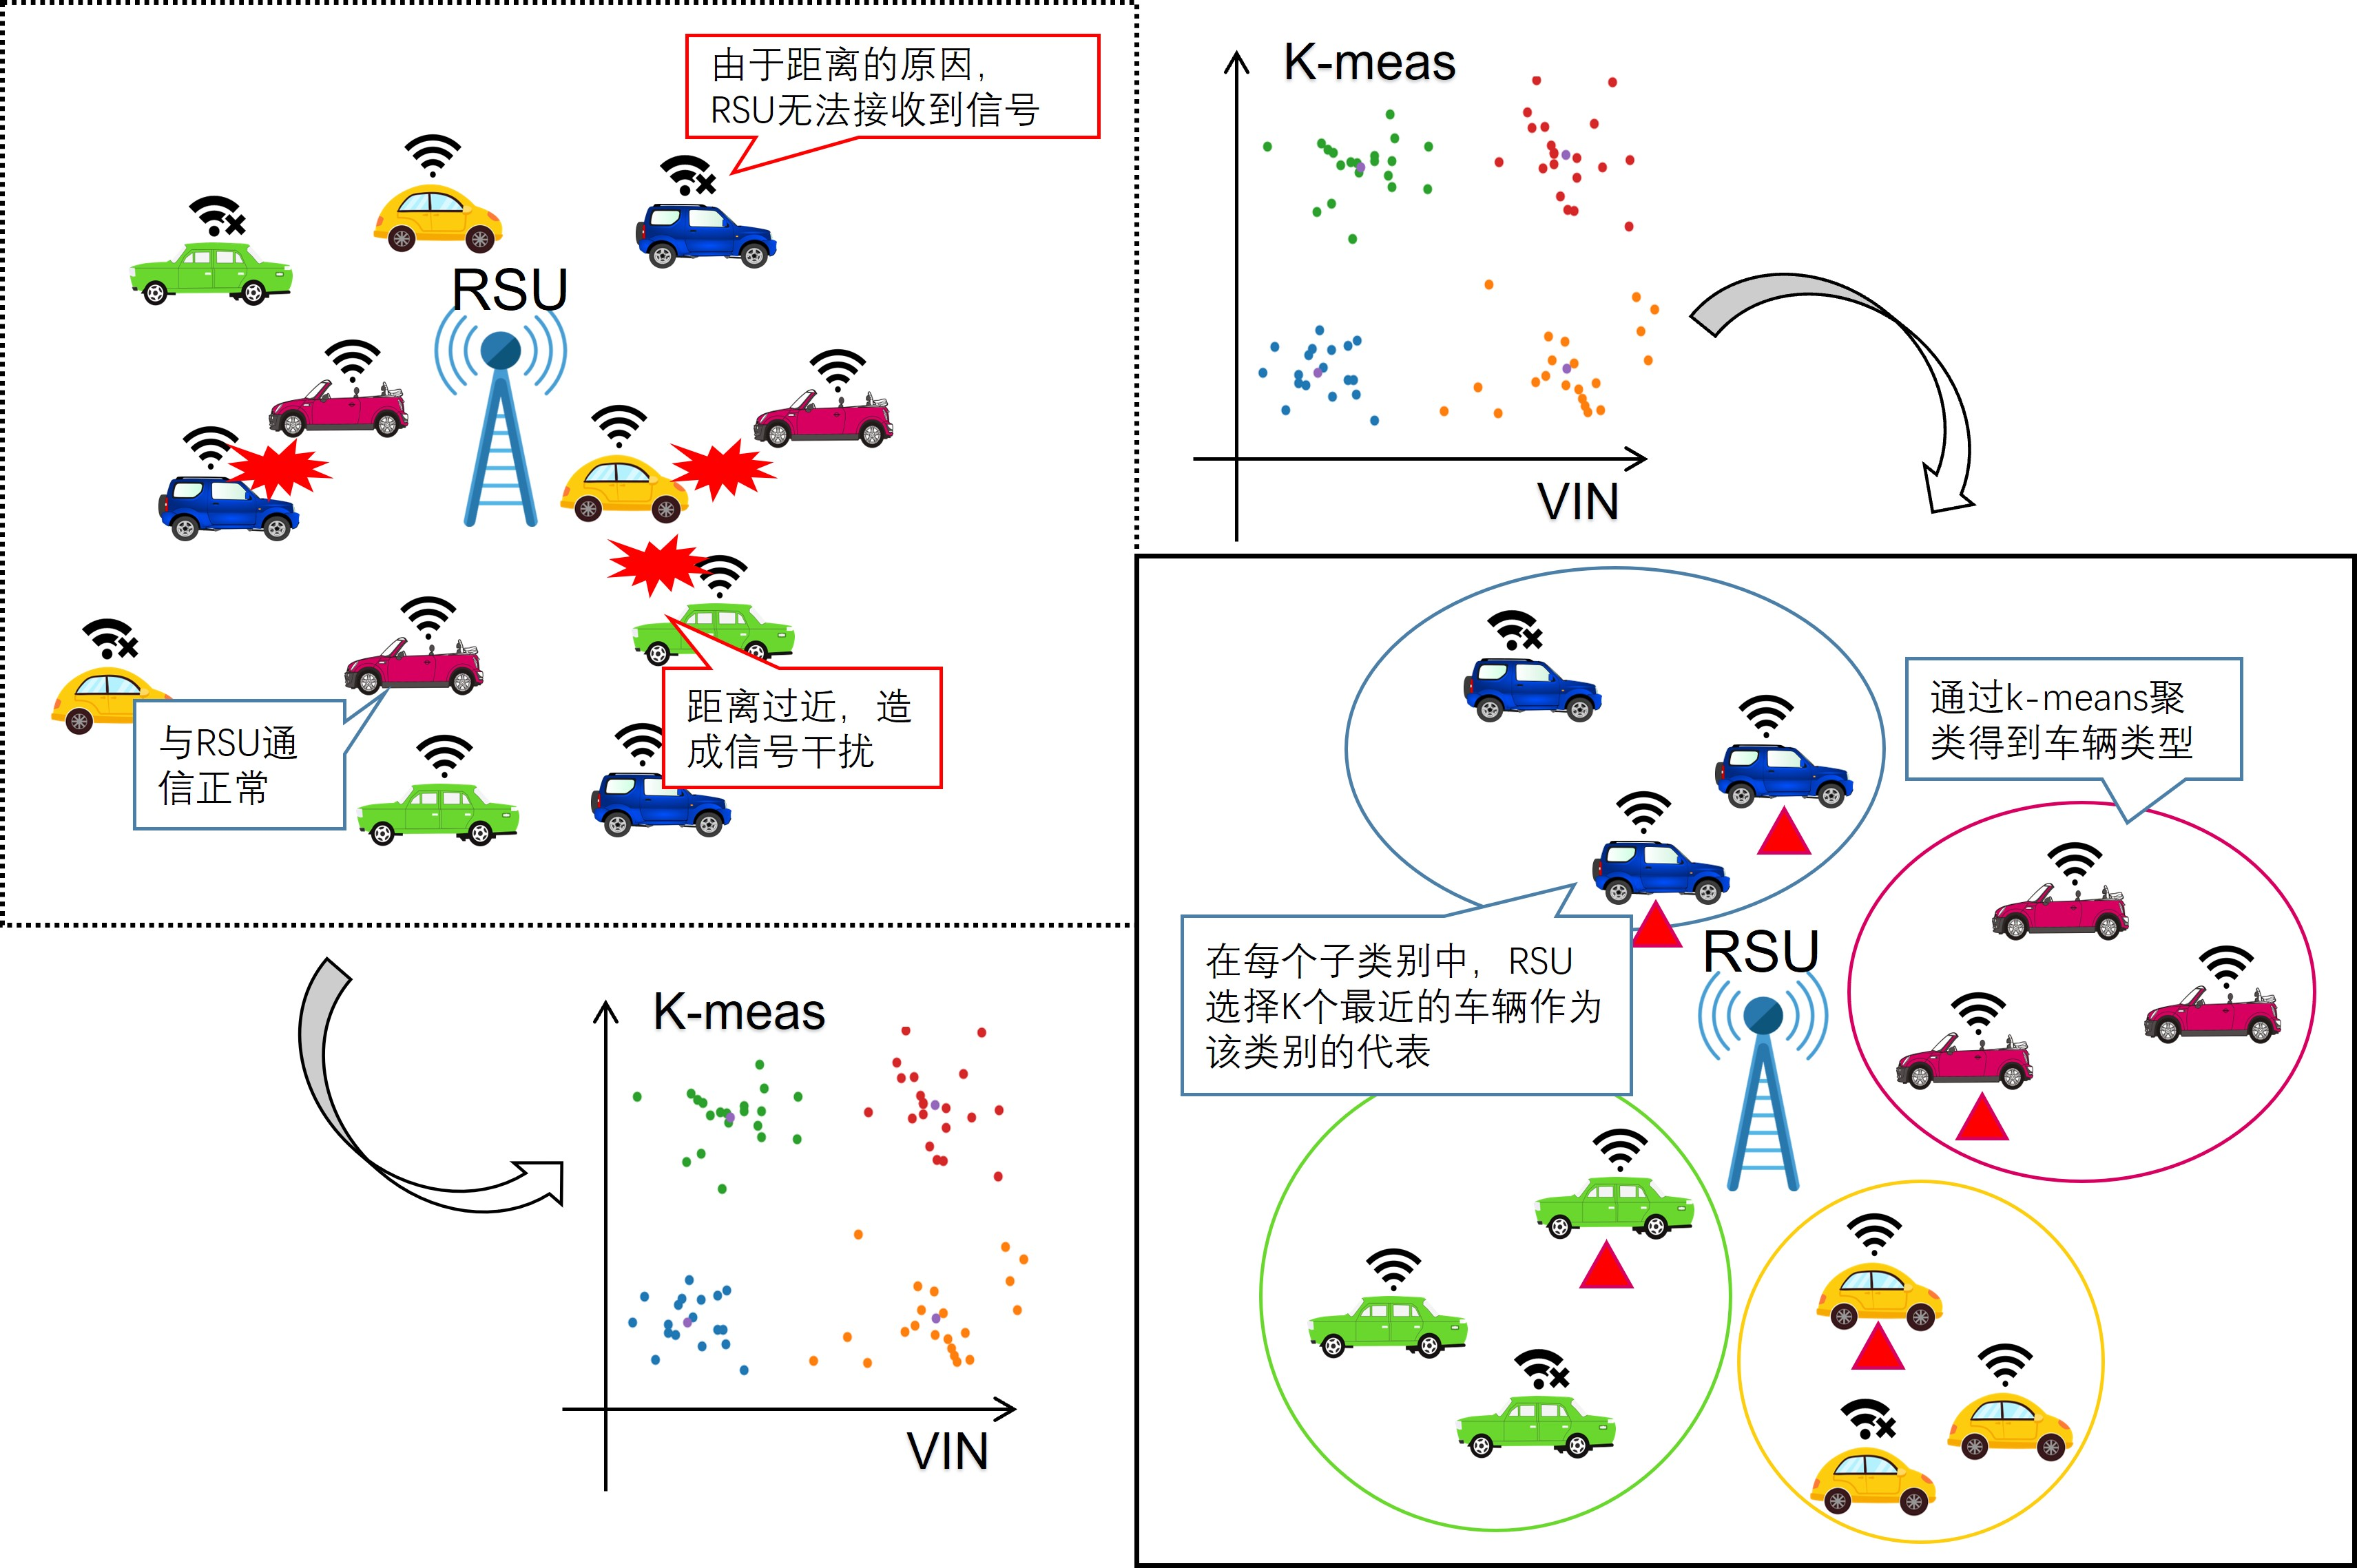
\includegraphics[scale=0.5]{figures/figure1.jpg}
    % \caption{FL-vgg16 Confusion Matrix}
    \caption{隐私保护计算的主要技术与三大隐私保证的对应关系}
    \label{fig:Cluster the cars in the region}
\end{figure}

\subsection{特征工程}

\subsection{汽车总线}

\section{基于迁移和特征工程的联邦学习CAN异常检测}\label{sec:HC}

本节提出了一种基于迁移和特征工程的联邦学习CAN异常检测的设计框架,该框架由三层组成,分别是:RSU(Road Side Unit,路侧单元)与MEC(Multi-access Edge Computing,多接入边缘计算)层,车与RSU层,车与车层。在该框架中,车联网中的车辆都装备了ECU(Electronic Control Unit,电子控制器单元)、OBUs和各种应用单元,实现了车辆之间和车辆与RSU之间的通信。MEC作为边缘计算的平台,提供了强大的计算能力,负责对来自不同RSU的联邦模型进行聚合更新和数据存储。RSU作为车联网的核心节点,负责本地模型的训练、数据的收集和清洗、异常检测的执行等功能,并将检测结果反馈给所属区域的车辆。当车辆进入RSU的服务范围时,可以主动向RSU发送检测请求,RSU则会收集车辆传输的CAN数据,并对其进行清洗和模型训练。

\subsection{车辆与RSU之间的数据传输}

\begin{figure}[htb]
\centering
    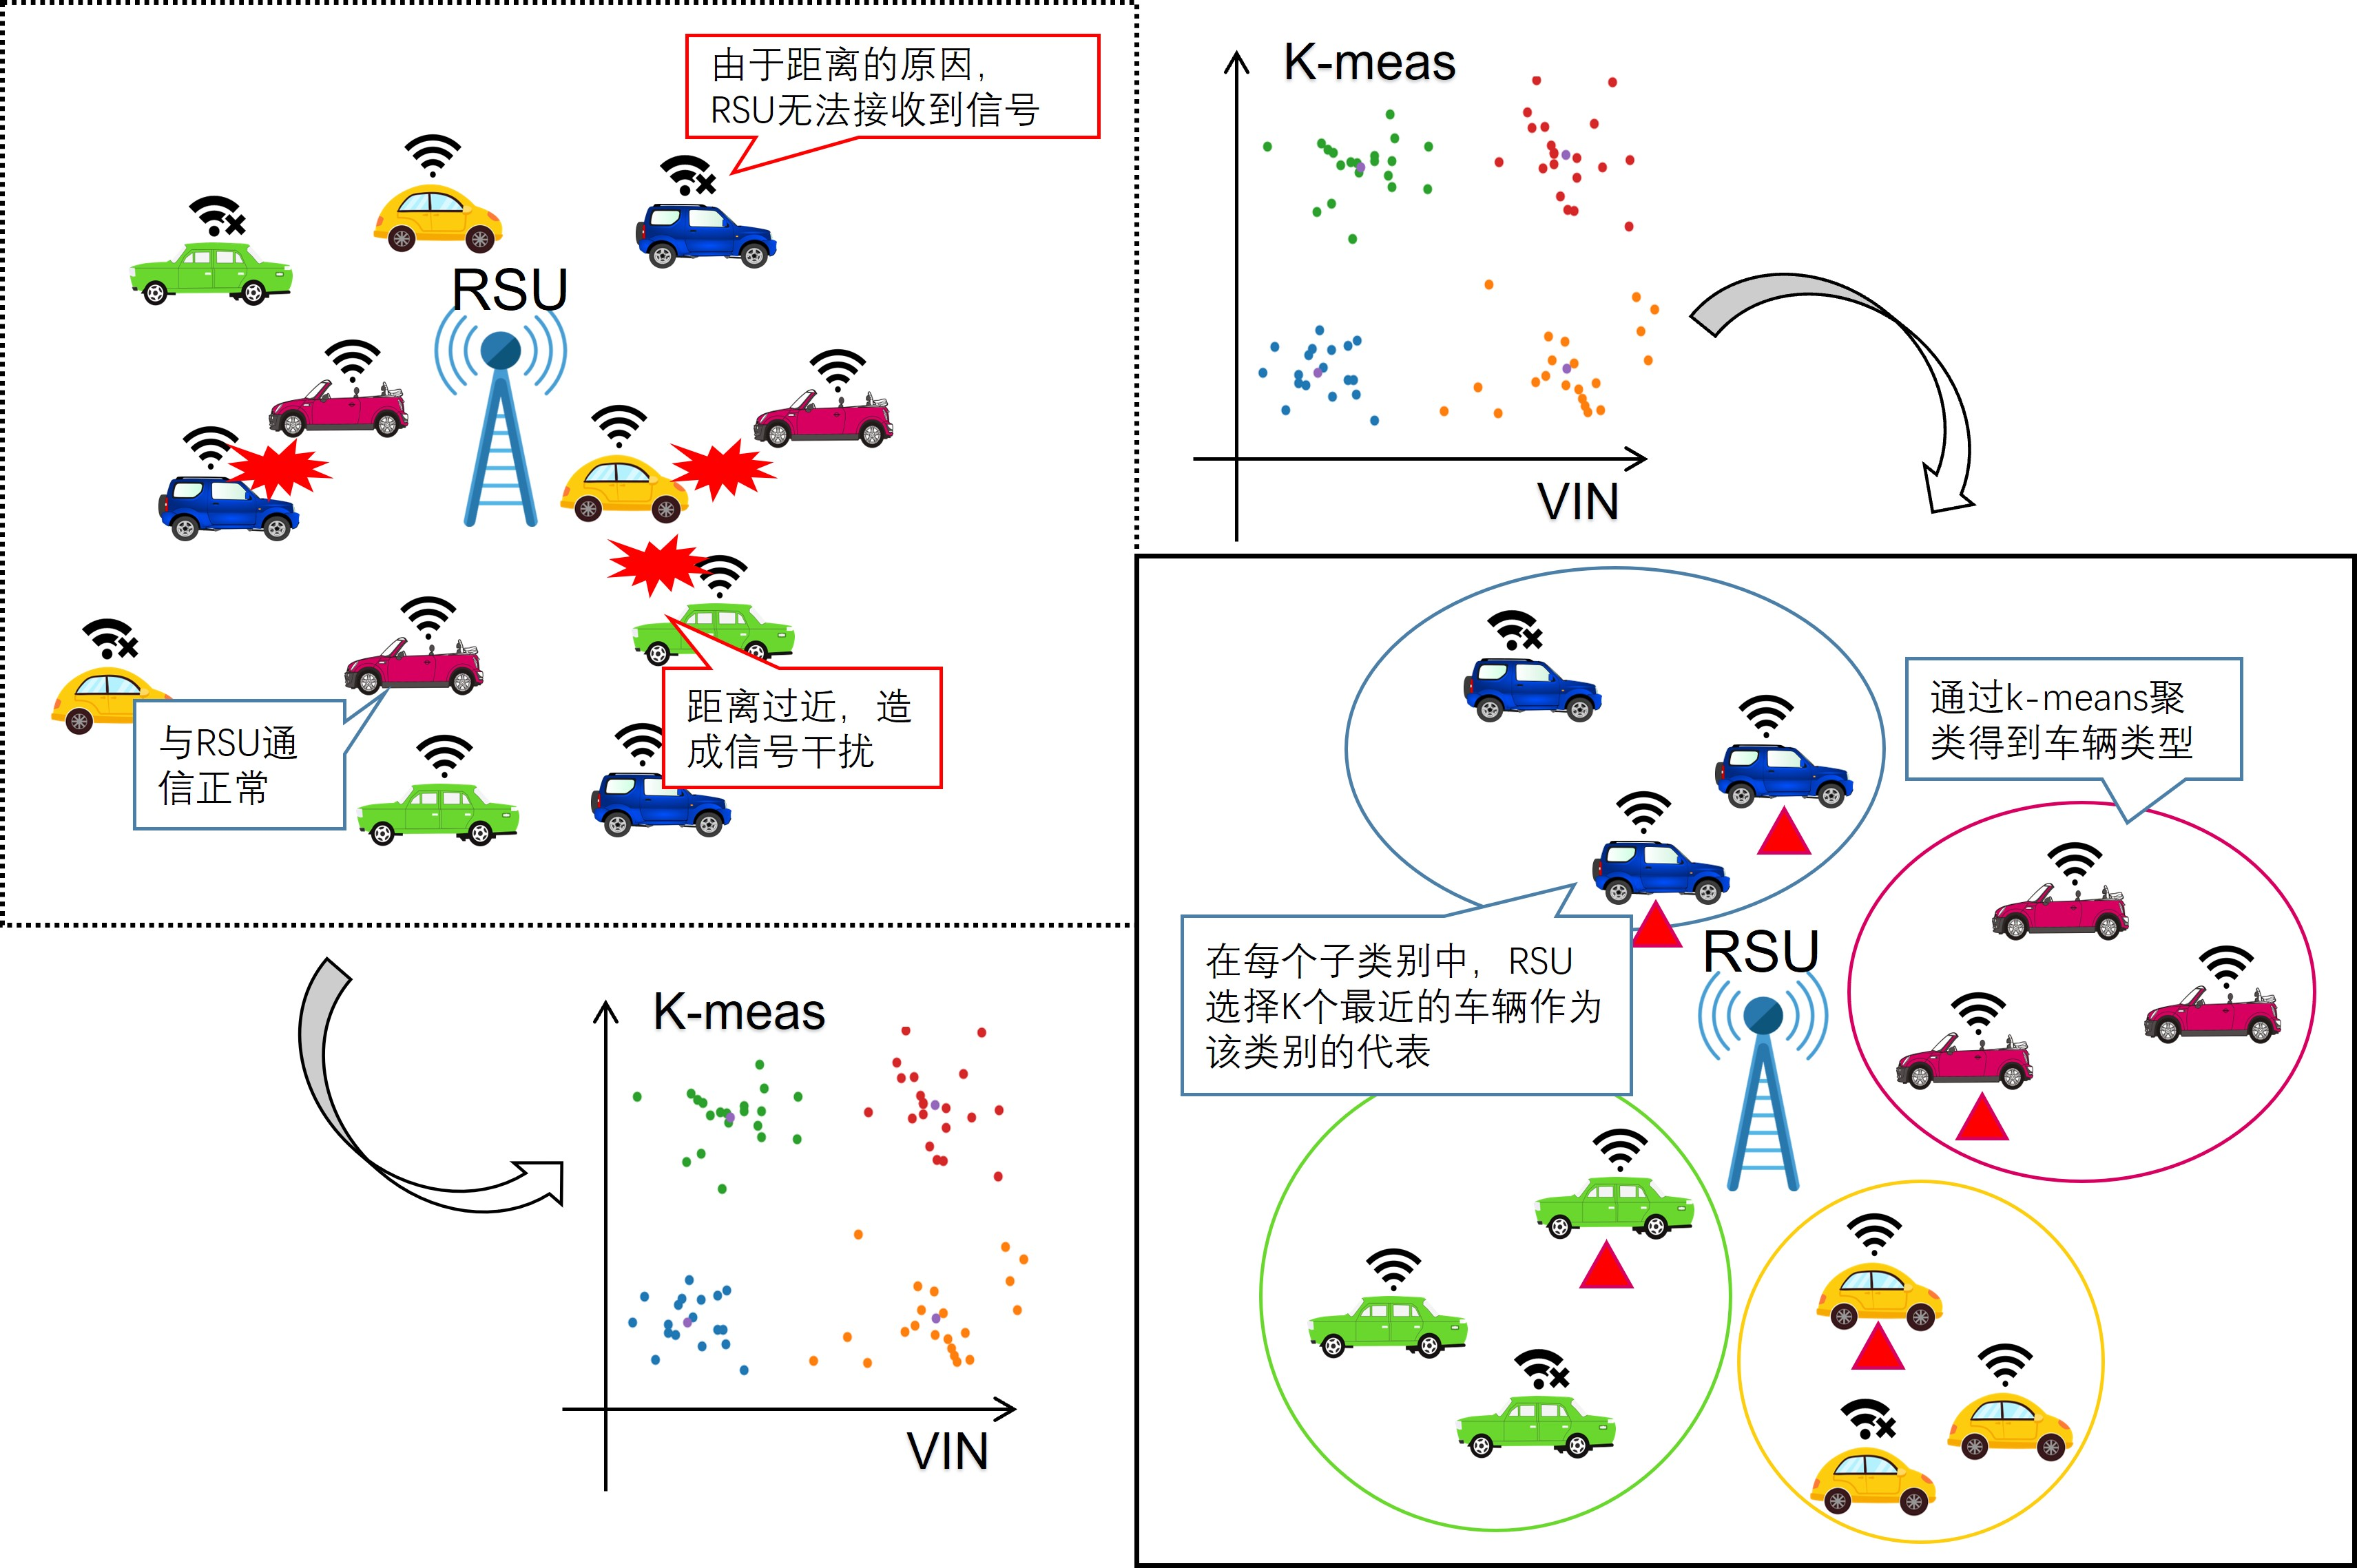
\includegraphics[scale=0.5]{figures/figure1.jpg}
    % \caption{FL-vgg16 Confusion Matrix}
    \caption{对区域内的车进行聚类}
    \label{fig:Cluster the cars in the region}
\end{figure}

本节考虑了车辆的动态性对联邦学习的影响,分析了车辆移动对RSU数据收集质量的影响(如传输延迟、消息碰撞或中断等)。由于入侵检测的目的是保护车辆的安全而不是RSU的安全,因此本节假设系统中的车辆都是积极的参与者,只有在自身条件允许时,才会将车辆识别码(Vehicle Identification Number,VIN)和位置信息传输给RSU。如图\ref{fig:Cluster the cars in the region}所示,RSU根据车辆识别码(Vehicle Identification Number,VIN)对区域内的车辆进行K-means聚类,假设可以将车辆分为$N$个类别,RSU根据欧几里得公式\ref{math:k-means},从每个类别中选择$k \geq 1$辆车作为本地数据来源,共计$kN$辆车。图中所示的情况是$N=4$,$k=2$。实际上,RSU将从每个类别中选择$max(1,k)$辆车,以保证每个类别至少有一辆车参与数据传输。

\begin{equation}
\begin{array}{l}
|AB|=\sqrt{(x_2-x_1)^2+(y_2-y)^2+(z_2-z_1)^2}\\
k\to\max(1,k)
\end{array}
\label{math:k-means}
\end{equation}

% 该模型将运行在智能车上,智能车的主要任务是自动巡航,因此不希望入侵检测占用大量的计算资源。轻量级的DL模型和欠采样技术通常应用于样本不均衡且数据集足够时,通过减少多数类的样本数以此获得类别均衡的数据集。当RSU接收到车辆的数据量超过自身内存的50\%时,会启动数据欠采样操作。欠采样方法集合中的Near Miss\cite{Zhang03}会根据多数类实例与少数类实例之间的距离来选择样本。该技术有三种版本,分别称为NearMiss-1,NearMiss-2和NearMiss-3。选用NearMiss-1时,会从多数类中选择那些与少数类中三个最接近示例的平均距离最小的示例。紧接着对数据进行非线性转换,这里本节选择的是yeo-Johnson\cite{yeo},其转化如公式\ref{math:yeo}所示。

% \begin{equation}
% \begin{aligned}
% x_i^{(\lambda )}=\begin{cases}
%  [(x_i+1)^\lambda -1] / \lambda  & \text{ if } \space  \lambda \ne 0,x_i \ge 0 \\
%  ln(x_i)+1  & \text{ if } \space  \lambda =  0,x_i \ge 0 \\
%  -[(-x_i+1)^{2-\lambda } -1] / (2-\lambda ) & \text{ if } \space  \lambda \ne 2,x_i <  0\\
%  -ln(-x_i+1) & \text{ if } \space  \lambda =  2,x_i < 0
% \end{cases}
% \label{math:yeo}
% \end{aligned}
% \end{equation}

% 文献\cite{A_Transfer_Learning_and_Optimized_CNN_Based_Intrusion_Detection_System_for_Internet_of_Vehicles}中选择的是quantile Transformer将数据转化为$0-1$中的均匀分布。然而,在机器学习领域中,具有正态分布形式的特征变量是大多数算法所期望的输入形式,幂转化可以将任何形式的分布转化为高斯分布,能够使方差稳定,减少偏度保持对称性。但是yeo-Johnson不能保证输出的值是一个0到1之间的值,所以在这之后本节又加上了如公式\ref{math:14}所示的min-max标准化。

为了在智能车上实现入侵检测,本节引入特征工程思想,首先,采用轻量级的DL模型和欠采样技术,以降低计算资源的消耗和解决样本不均衡的问题。欠采样技术的原理是通过减少多数类的样本数量,使数据集的类别分布更加平衡。本节引入特征学习思想,首先使用一种基于距离的欠采样方法,即Near Miss\cite{Zhang03},该方法有三种版本,分别是NearMiss-1,NearMiss-2和NearMiss-3。本节选择了NearMiss-1,其算法是从多数类中选择那些与少数类中最近的三个样本的平均距离最小的样本。当RSU接收到的车辆数据量超过其内存的50\%时,就会对数据进行欠采样处理。其次,为了使数据更适合DL模型的输入,本节还对数据进行了非线性变换,即yeo-Johnson\cite{yeo}变换,其公式如下:

\begin{equation}
\begin{aligned}
x_i^{(\lambda )}=\begin{cases}
 [(x_i+1)^\lambda -1] / \lambda  & \text{ if } \space  \lambda \ne 0,x_i \ge 0 \\
 ln(x_i)+1  & \text{ if } \space  \lambda =  0,x_i \ge 0 \\
 -[(-x_i+1)^{2-\lambda } -1] / (2-\lambda ) & \text{ if } \space  \lambda \ne 2,x_i <  0\\
 -ln(-x_i+1) & \text{ if } \space  \lambda =  2,x_i < 0
\end{cases}
\label{math:yeo}
\end{aligned}
\end{equation}

yeo-Johnson变换是一种幂变换,可以将任何分布的数据转换为正态分布,从而使数据的方差稳定,减少偏度,保持对称性。这些特性有利于提高机器学习算法的性能。然而,yeo-Johnson变换不能保证输出的数据在$0-1$之间,因此本节在变换后还对数据进行了min-max标准化,其公式如下:

\begin{equation}
\begin{aligned}
x_i'=\frac{x_i-\min(x)}{\max(x)-\min(x)}
\label{math:14}
\end{aligned}
\end{equation}

最后,使用min-max标准化将数据缩放到$0-1$之间,使数据的范围更加一致,避免因为数据的量纲不同而影响模型的训练效果。文献\cite{A_Transfer_Learning_and_Optimized_CNN_Based_Intrusion_Detection_System_for_Internet_of_Vehicles}中使用了quantile Transformer将数据转换为$0-1$之间的均匀分布,但本节认为正态分布更符合数据的实际情况,此时,所有的CAN数据都将落到0-255之前,由于数据的特殊性,可以将其由十六进制的字节码转化为图片数据,详细见本文的实验设置部分。

\subsection{RSU的DL模型选择}

\begin{figure}[htb]
\centering
    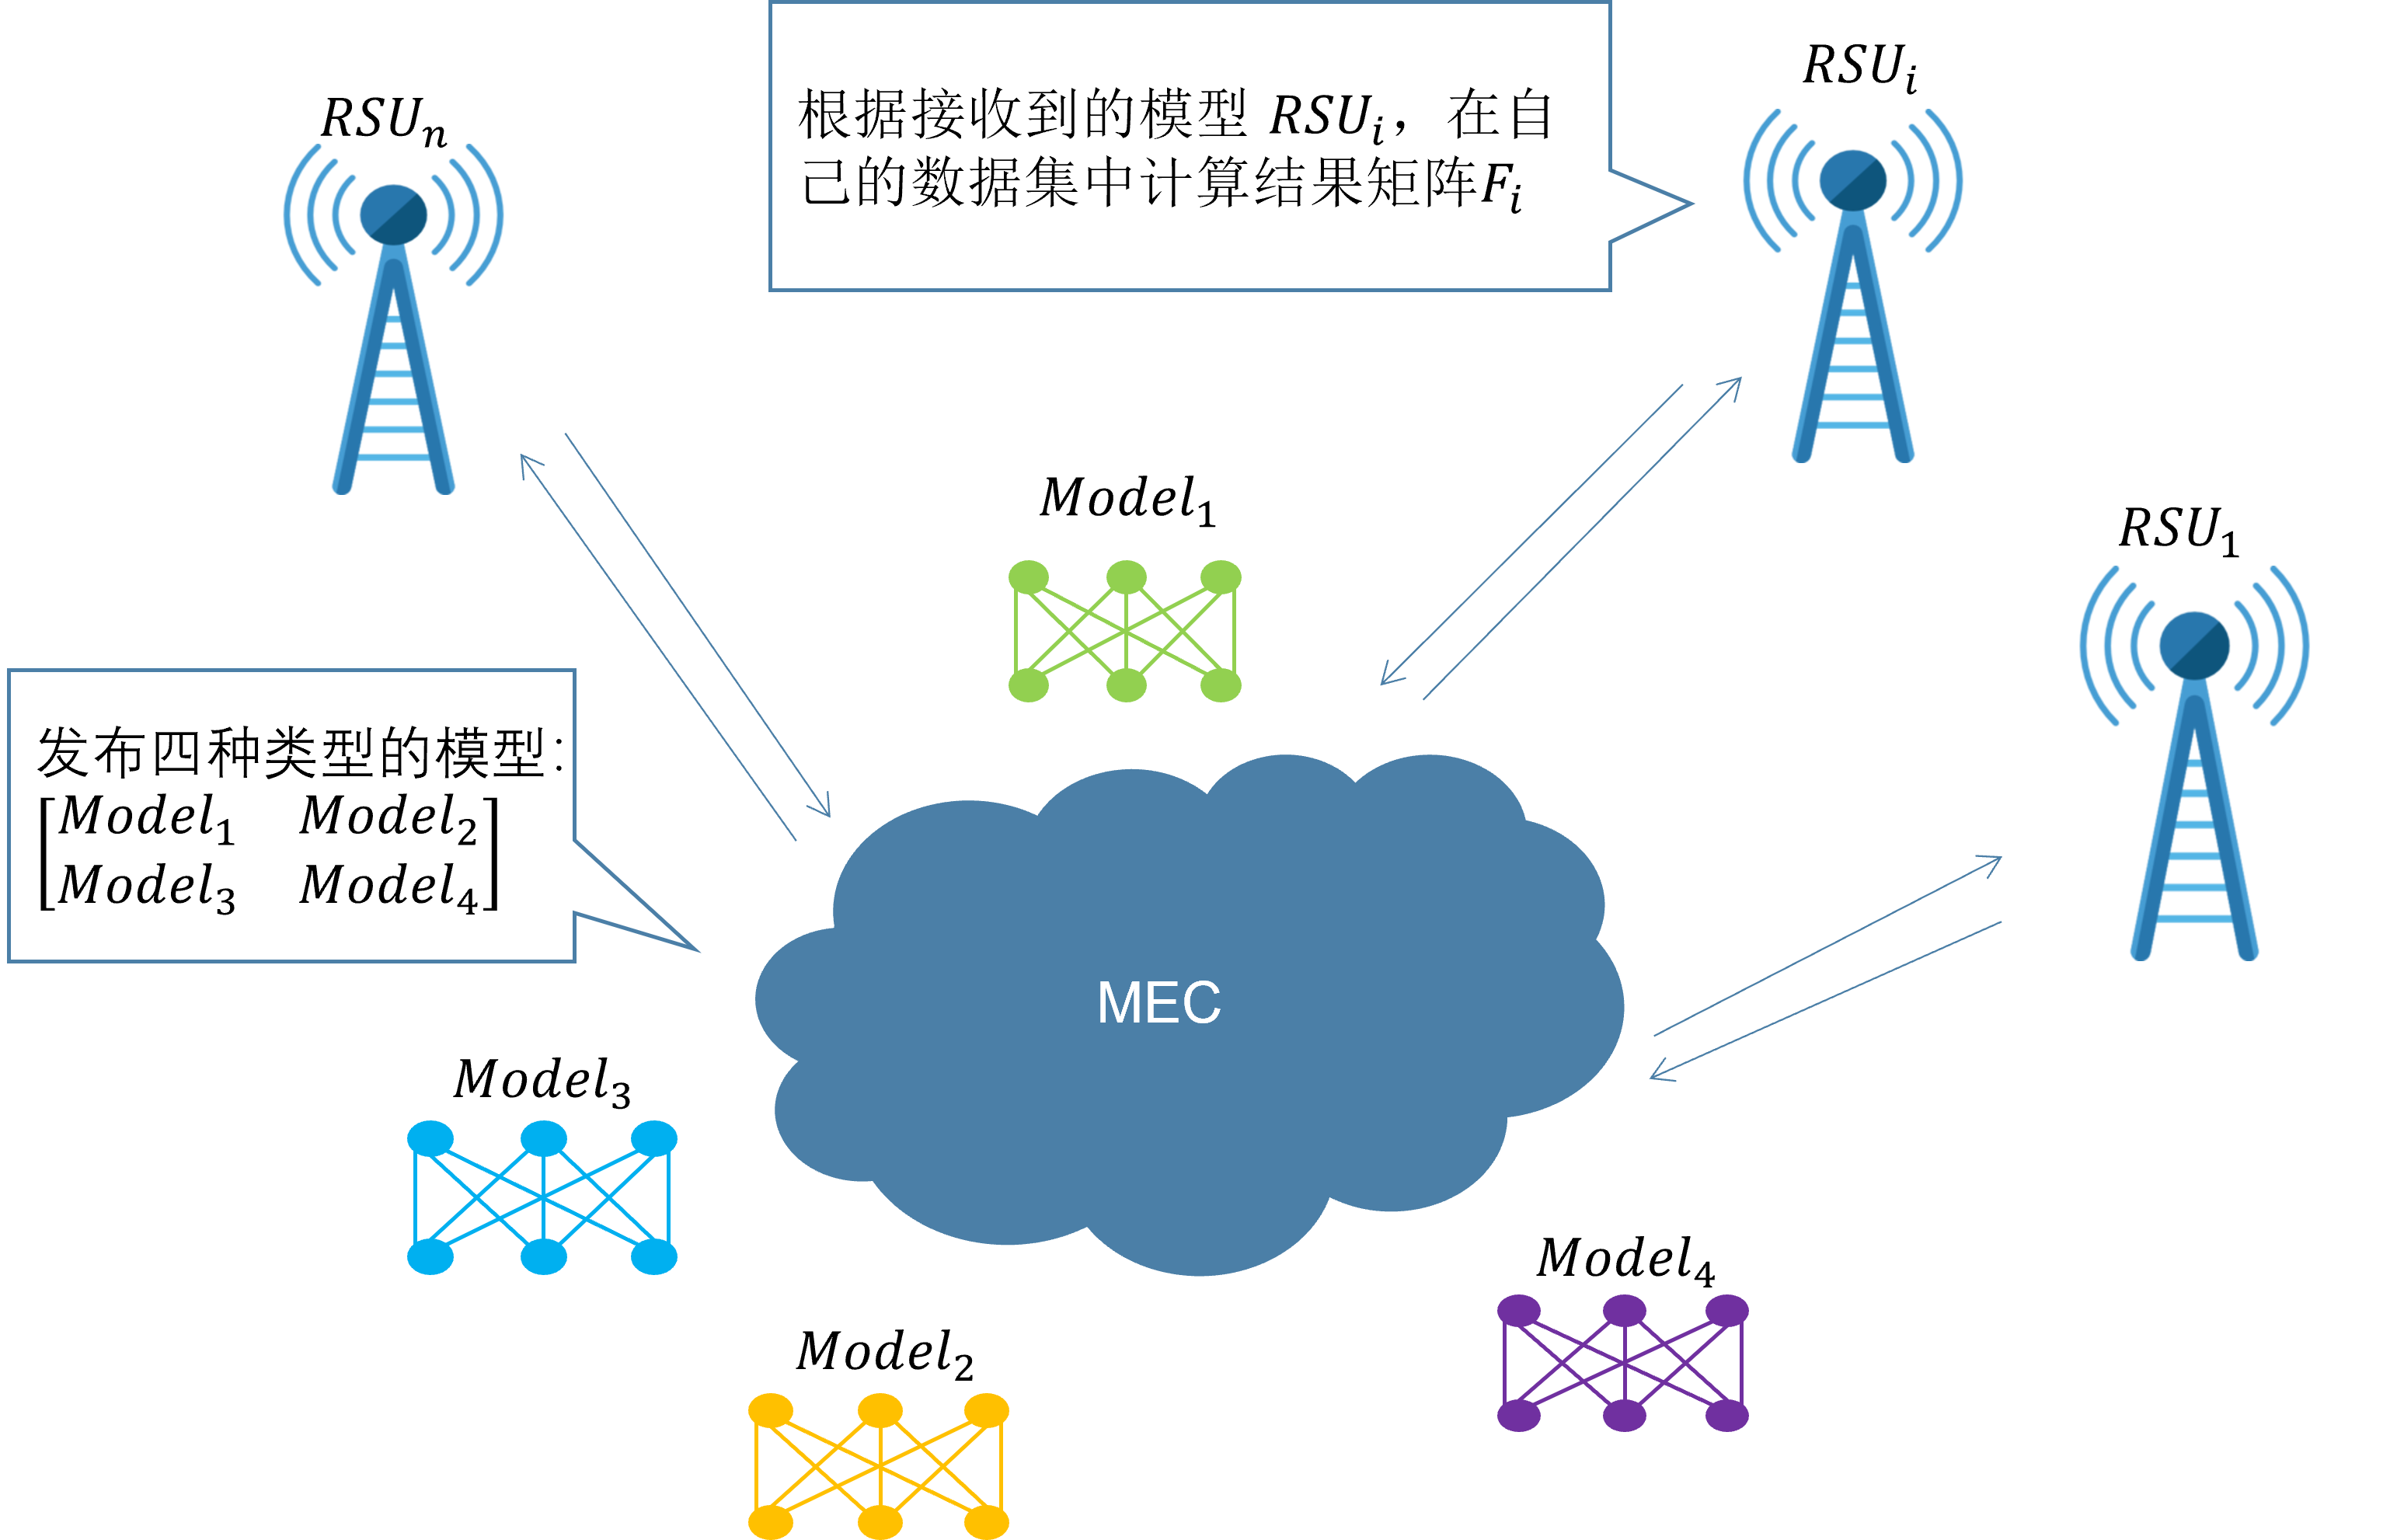
\includegraphics[scale=0.6]{figures/figure2.png}
    % \caption{FL-vgg16 Confusion Matrix}
    \caption{对区域内的车进行聚类}
    \label{fig:Cluster the cars in the region}
\end{figure}

本节研究了在移动边缘计算(MEC)环境下,如何为不同类型的路侧单元(RSU)提供个性化的深度学习(DL)模型,以实现车辆入侵检测的联邦学习任务。MEC作为系统的中心节点,负责模型的聚合与分发。由于RSU的种类繁多,不同厂商生产的RSU所配备的软硬件资源不同,同时,不同地点的RSU接收的CAN数据量也不同,例如位于城市主干道上的RSU接收的数据将远远多于乡镇等支线上的数据。因此,本节需要为不同地方的RSU提供更加适合其数据特征和资源条件的模型。

为了解决这一问题,本节引入了迁移学习的思想,利用多个领域的共享知识来建立有效的模型。迁移学习的优势在于,它可以利用已有的大量数据训练出一个好的模型,然后将其作为联邦学习任务的初始模型,从而减少训练时间和资源消耗。本节在MEC中集成了四类预训练后的DL模型,分别是CNN、VGG16、ResNet18、AlexNet。在系统启动的初期,MEC会将这四类模型下发给选中的$\alpha$个RSUs。

设第$i$个RSU为$R_i$,则$R_i$将采用四款模型在本地数据集上进行训练,将模型收敛后得到的更新梯度$g_k,k\in[1,4]$和F1得分$f_k,k \in[1,4]$返回给MEC,其中$g_k$与$f_k$一一对应,表示第$k$个模型训练得到的值。F1得分是一种衡量模型分类性能的指标,其计算公式如公式\ref{math:15}所示。$F'_i$表示为$R_i$的临时结果矩阵,则$F'_i$如公式\ref{math:7}所示。
\begin{equation}
    \begin{aligned}
    F'_i=\begin{bmatrix} f_1 & g_1 \\ f_2 & g_2\\f_3 &  g_3 \\f_4 &  g_4 \end{bmatrix}
    \end{aligned}
    \label{math:7}
\end{equation}
为了选择最适合$R_i$的模型,本节定义了一个系数矩阵$\theta $,设定四个资源相关参数:最大训练时间$t$,最小loss值$l$,模型大小$u$,训练所需CPU性能$c$。对于CNN、VGG16、ResNet18、AlexNet这四类模型来说,最大训练时间$t$,模型大小$u$,训练所需CPU性能$c$都各不相同,而最小loss值$l$均一样。同时定义一个放缩函数$\mathcal{F}, $使得$\mathcal{F}(t),\mathcal{F}(l),\mathcal{F}(u),\mathcal{F}(c) \in (0,1]$,由于本节希望这四个值都越小越好,则可以得到公式\ref{math:11}:
\begin{equation}
    \begin{aligned}
    \theta =\begin{bmatrix}
     \mathcal{F}(t_1)\mathcal{F}(l)\mathcal{F}(u_1)\mathcal{F}(c_1) \\
     \mathcal{F}(t_2)\mathcal{F}(l)\mathcal{F}(u_2)\mathcal{F}(c_2) \\
     \mathcal{F}(t_3)\mathcal{F}(l)\mathcal{F}(u_3)\mathcal{F}(c_3) \\
     \mathcal{F}(t_4)\mathcal{F}(l)\mathcal{F}(u_4)\mathcal{F}(c_4) 
    \end{bmatrix}=\begin{bmatrix}
     \theta_1 \\ \theta_2 \\ \theta_3 \\  \theta_4
    \end{bmatrix}
    \end{aligned} 
    \label{math:11}
\end{equation}
因此最终的结果矩阵$F_i$如公式\ref{math:12}所示:
\begin{equation}
    \begin{aligned}
    F_i=\begin{bmatrix} f_1/\theta_1  & g_1 \\ f_2/\theta_2  & g_2\\f_3/\theta_3  &  g_3 \\f_4/\theta_4 &  g_4 \end{bmatrix}
    \end{aligned} \label{math:12}
\end{equation}

\subsection{MEC的联邦学习}

\begin{figure}[htb]
\centering
    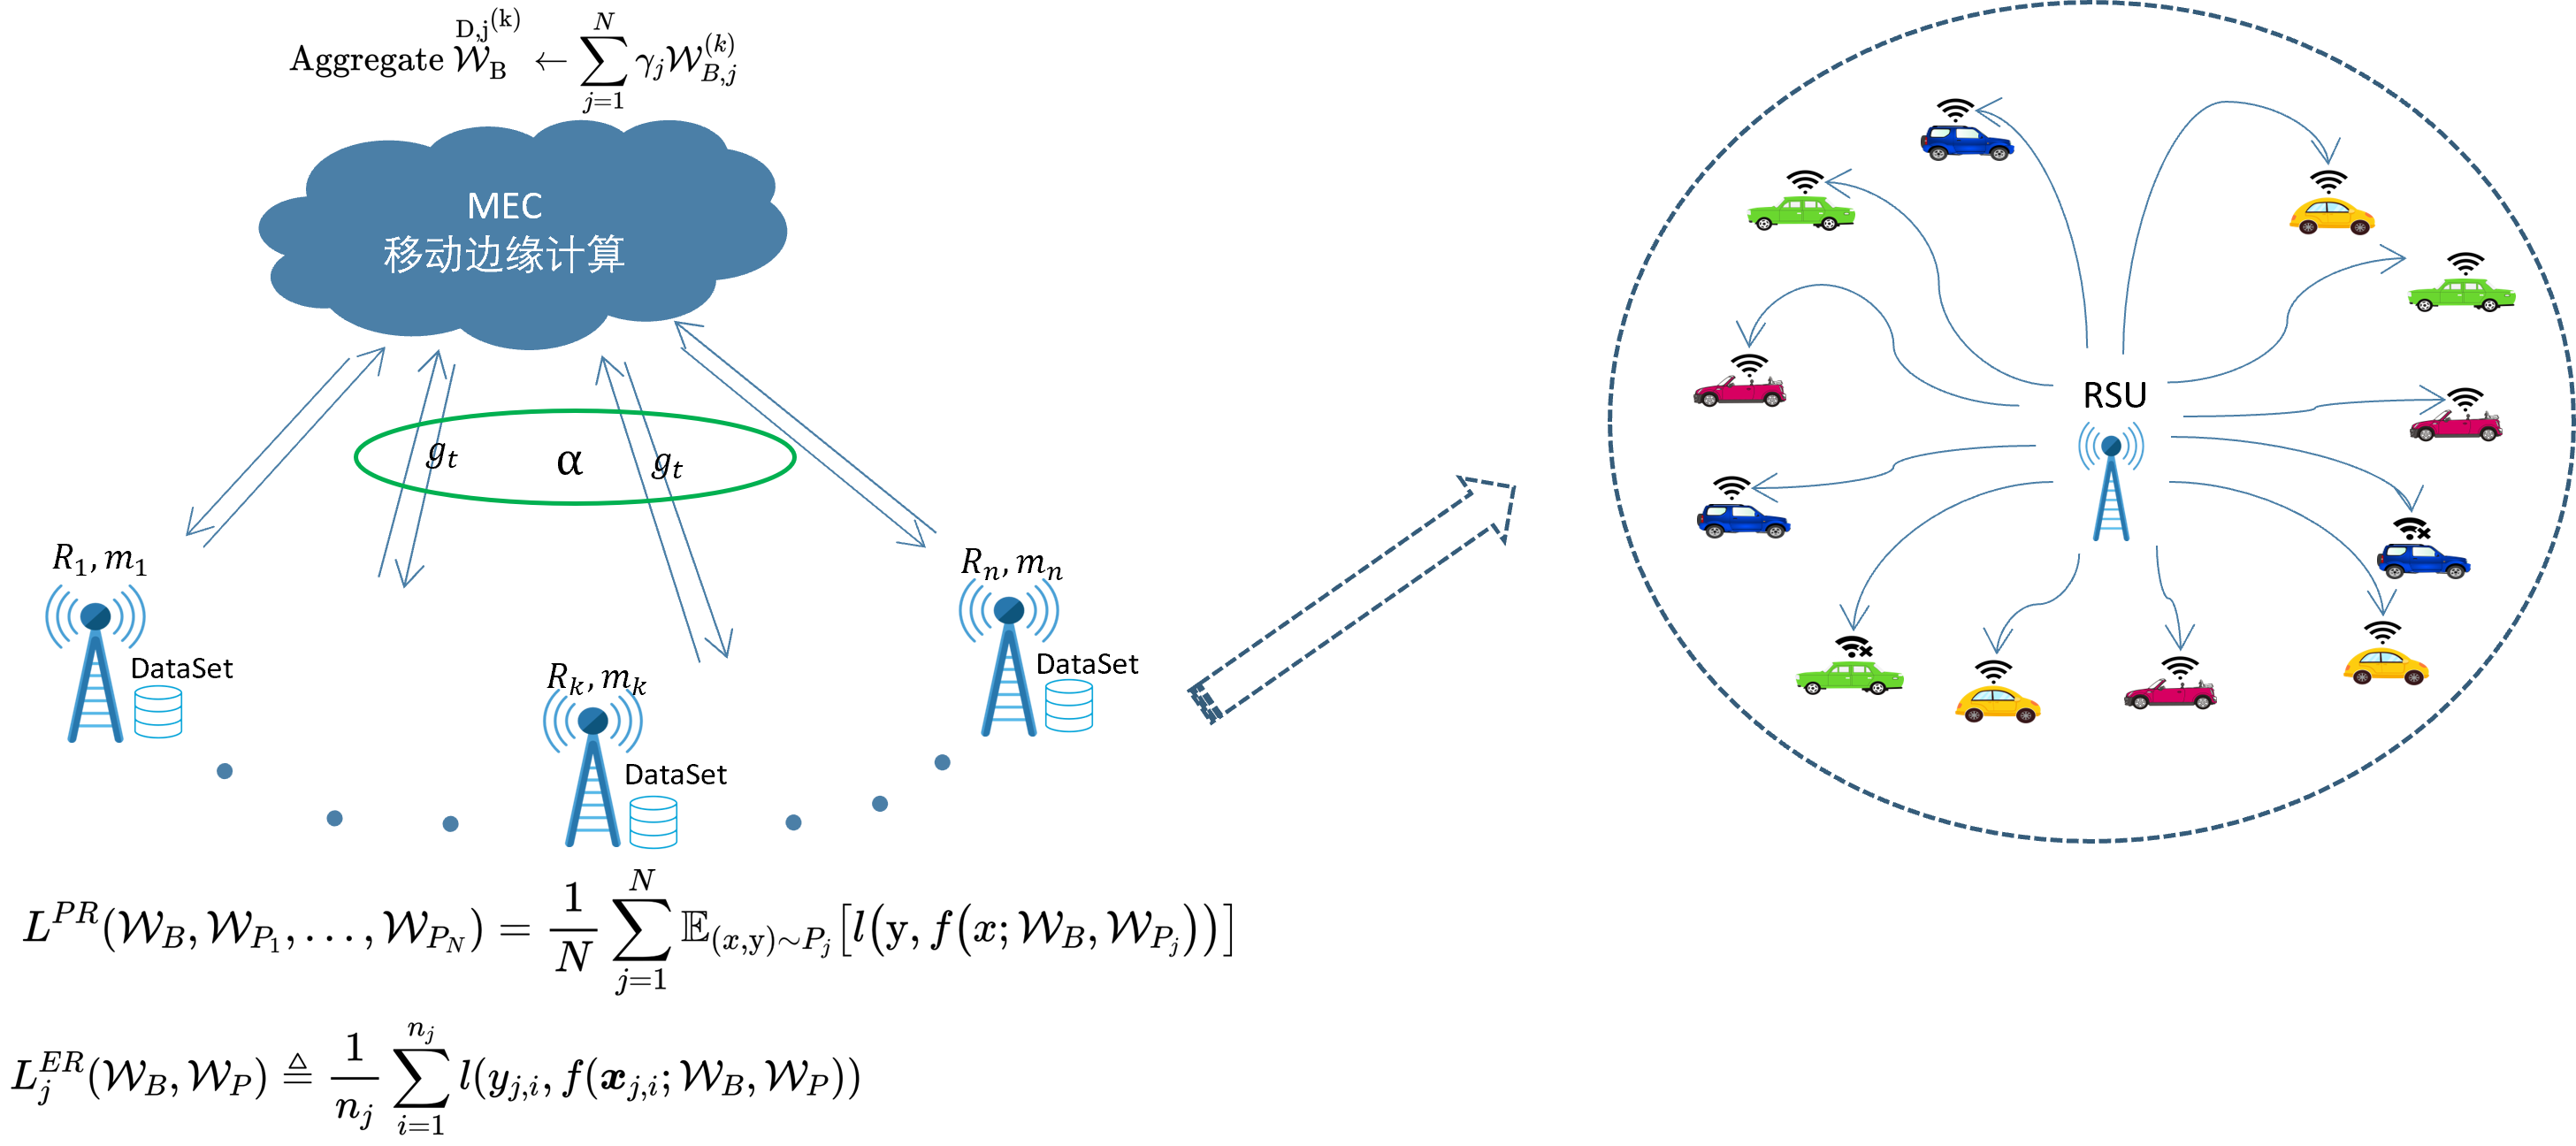
\includegraphics[scale=0.65]{figures/chapter3/chapter3.png}
    % \caption{FL-vgg16 Confusion Matrix}
    \caption{对RSU进行聚类}
    \label{fig:Cluster the cars in the region}
\end{figure}

本节研究了在移动边缘计算(MEC)环境下,如何为不同类型的路侧单元(RSU)提供个性化的深度学习(DL)模型,以实现车辆入侵检测的联邦学习任务。MEC作为系统的中心节点,负责模型的聚合与分发。MEC收到所有RSU传来的结果矩阵后,会得到集合$F=\{F_1,F_2,\dots,F_n\}$。MEC将根据$F$进行二次聚类,将区域内的RSU分配到四类模型中。
% 对于每一个小分类,使用FedPer\cite{Federated_learning_with_personalization_layers}算法,进行全局模型训练。FedPer算法的核心思想是将待训练的模型分为“基础+个性化层”,基础层可以作为共享层捕捉群体的智慧,而个性化层可以作为任务特定层捕捉客户端特定方面。

取$F_{sum}$中最大值$F_{s_k}= MAX(F_{sum})$对应的模型作为联邦学习系统中的最终模型$M_{select}$,同时得到对应梯度$ g_{select}= G_{s_k}$。设第$t$轮,MEC上的全局模型为$M_{i_t}$,参与更新的RSU集合为$R=\{R_1,R_2,\dots,R_n\}$,$R_k \in R$,对应的数据索引集大小为$m_k$,所有参与方的数据集总样本数为$m=\sum_{k=1}^{n}m_k$。MEC中设定有参与联邦学习的RSU比例$\alpha \in (0,1]$,那么参与第$t$轮迭代的RSU个数为$max(\alpha n,1)\to m$。$\beta$为学习率,损失函数为$H_k=\frac{1}{B}\sum_{i \in b }h_i(w)  $,$B$为训练批次大小,$b $为$R_k$中一个批次中的数据索引,则联邦学习的总损失函数为$H(w)=\sum_{k=1}^{m} \frac{m_k}{m}H_k(w,b)$。$R_k$使用MEC下发的模型梯度$g_t$在$ M_{select}$上进行模型初始化$g_t \to g_{t+1}^k$,然后将自身数据集分为大小为$B$的若干批次,每一次迭代进行局部模型参数更新$g_{t+1}^{k}-\beta H_{k}\to g_{t+1}^{k}$,然后将更新好的局部模型参数$g_{t+1}^k \in G_{s_k}$传输给MEC。MEC将聚合所有的参数$g_{t+1}=\sum_{k=1}^{n}\frac{m_k}{m}g_{t+1}^k$,再将结果发送回所有参与训练的RSU。整个系统将一直重复这个过程,直到$g_{t+1}$收敛。

MEC将持续监控达到收敛状态的全局模型,一旦发现由于车辆移动导致的RSU收集到的CAN数据变化、特殊RSU离线等原因导致模型检测性能下降,将再次重启整个联邦学习过程。

\section{基于迁移和特征工程的联邦学习CAN异常检测实验}

\subsection{实验设置和实现细节}

\textbf{数据集和实验环境的介绍。}\label{subsection:Dataset_and_experimental_environment}本节采用了Car-Hacking数据集作为实验数据,该数据集包含了四种常见的车辆内部攻击类型,即DoS攻击、模糊攻击、驱动装置欺骗和RPM仪表欺骗。这些攻击类型都是通过OBD-II端口对真实的CAN流量进行入侵而产生的,具有较高的真实性和可信度。Car-Hacking数据集目前是车辆入侵检测领域的一个重要的基准数据集,被广泛用于评估不同的检测方法的性能。本节在一台安装了Windows 11操作系统的计算机上,模拟了RSU对本地数据集的预处理过程。该计算机的配置为Intel Core i5-8300H CPU @ 2.30GHz处理器和24.0 GB内存。由于Car-Hacking数据集的总体规模较大(902.01 MB),本节只选取了其中的5\%作为实验数据,相当于一个RSU覆盖范围内的车辆CAN数据,共有818,440条记录。图\ref{fig:data type distribution}显示了实验数据的类别分布情况,可以看出正常流量占了85.5\%,而异常流量占了14.5\%,存在一定程度的数据不平衡问题。

\begin{figure}[htb]
    \centering
    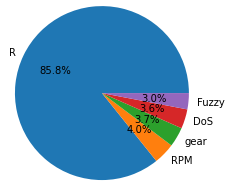
\includegraphics[width=0.50\textwidth]{figures/Data type distribution.png}
    \caption{数据类型分布图}
    \label{fig:data type distribution}
\end{figure} 

% 图\ref{fig:Histogram of raw data distribution}展示的是原始数据的分布情况,横坐标为特征的数值,纵坐标为9个特征的数量。可以发现特征"car id"与其他特征的数值差异大。因此本文将一次进行章节\ref{subsection:Data_undersampling}、\ref{subsection:Nonlinear_transformation _of_data}和\ref{subsection:Generating_images}中所述的操作。
% \begin{figure}[htb]
%     \centering
%     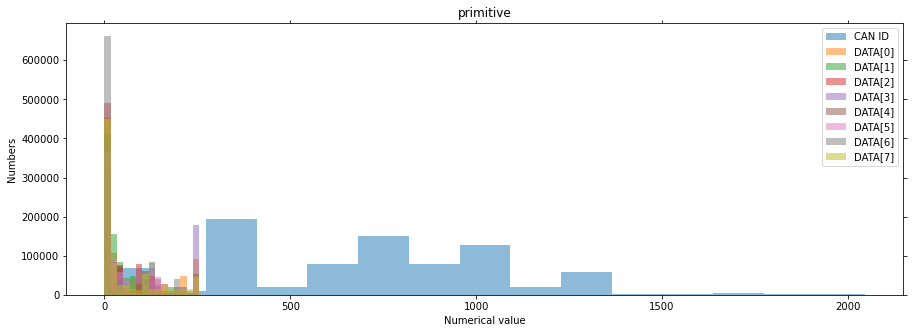
\includegraphics[width=0.8 \textwidth]{figures/Histogram of raw data distribution.png}
%     \caption{Histogram of raw data distribution}
%     \label{fig:Histogram of raw data distribution}
% \end{figure}

\textbf{评价指标及其影响因素。}\label{subsection:Evaluation_metrics_and_influencing_factors}本节针对Federated Learning(FL)中的性能问题,如准确性、延迟和资源约束等,选择了合适的评价指标,并分析了影响这些指标的因素。首先,采用F1值作为评价分类模型的准确性的指标,其定义如公式\ref{math:15}所示。F1值是精确率和召回率的调和平均,能够综合反映模型的分类效果,其值越接近1,表示模型的准确性越高。其次,本文不仅在单一深度学习模型上进行训练,还利用模型融合的方法,结合不同模型的优势,进一步提升系统的分类准确性。最后,本节考虑了入侵检测的场景和需求,将RSU作为模型的执行者,将车辆作为模型的请求者,分析了影响系统延迟和资源消耗的因素。系统延迟$T$主要由数据预处理时间$t_p$和模型训练时间$t_t$构成,而资源消耗主要包括模型的大小和算力。本节将对不同的模型进行比较和筛选,以找出适合在RSU上运行的模型。

\begin{equation}
\begin{aligned}
F1=(\frac{2+\frac{FP}{TP}+\frac{FN}{TP}}{2})^{-1}
\label{math:15}
\end{aligned}
\end{equation}

\begin{equation}
\begin{aligned}
T=t_p+t_t
\label{math:16}
\end{aligned}
\end{equation}

\textbf{数据欠采样方法的比较分析。}\label{subsection:Data_undersampling}为了解决数据不平衡问题,本节对六种数据欠采样方法进行了实验分析,分别是Random UnderSampler(RUS)、Tomek Links(TL)、One-Sided Selection(OSS)、Condensed Nearest Neighbour(CNN)、Edited Nearest Neighbours(ENN)和All-KNN,并以Near Miss(NM)作为对照组。表\ref{table:Sampling scheme and its running result}展示了各种方法的运行时间和欠采样后的样本数。从表中可以看出,基于压缩最近邻和推导的方法(CNN和OSS)在欠采样效果上较差,而基于最近邻和Tomek Links的方法(ENN、All-KNN和TL)虽然有一定的改善,但仍未能有效地解决数据不平衡问题。RUS方法虽然运行速度最快,但它只是简单地对多数类样本进行随机抽样,导致欠采样后的样本分布与原始数据分布不一致,容易造成欠拟合现象,不适用于Car-Hacking这种正负样本比例极端不平衡的数据集。综上所述,本节选择了NM方法作为最佳的欠采样方法。

\begin{table*}[!ht]
    \centering
    \caption{Sampling scheme and its running result}
    \begin{tabular}{ccccccccc}
    \hline
        \textbf{} & \textbf{Original} & \textbf{RUS} & \textbf{NM} & \textbf{TL} & \textbf{OSS} & \textbf{CNN} & \textbf{ENN} & \textbf{Allknn} \\ \hline
        $t_p$(s)  & ~ & 5.29 & 120.59 & 729.34 & 714.11 & 3526.61 & 802.87 & 2211.79 \\ 
        R & 701832 & 24624 & 24624 & 701831 & 682795 & 60 & 701824 & 701824 \\ 
        DOS & 29501 & 24624 & 24624 & 29501 & 1 & 1 & 29501 & 29501 \\ 
        RPM & 32539 & 24624 & 24624 & 32539 & 0 & 1 & 32539 & 32539 \\ 
        Gear & 29944 & 24624 & 24624 & 29944 & 1 & 1 & 29944 & 29944 \\ 
        Fuzzy & 24624 & 24624 & 24624 & 24624 & 24624 & 24624 & 24624 & 24624 \\ \hline
    \end{tabular}
    \label{table:Sampling scheme and its running result}
\end{table*}

\textbf{数据非线性转化的效果分析。}\label{subsection:Nonlinear_transformation _of_data}为了提高数据的正态性,本节对经过Near Miss降采样后的数据进行了两种不同的幂转化,分别是quantile Transformer转化和yeo-Johnson幂转化,并对转化后的数据进行了min-max标准化。图\ref{fig:Two kinds of histograms after power transformation}显示了转化后的数据直方图,从中可以发现,quantile Transformer转化能够使数据呈现出明显的高斯分布,而yeo-Johnson幂转化则没有达到这样的效果。因此,本节选择了quantile Transformer转化作为最佳的非线性转化方法。

\begin{figure}[htb]
    \centering
    \subfigure[yeo-johnson-nearmiss-maxmin]{
        \begin{minipage}[b]{1\linewidth}
        \centering
        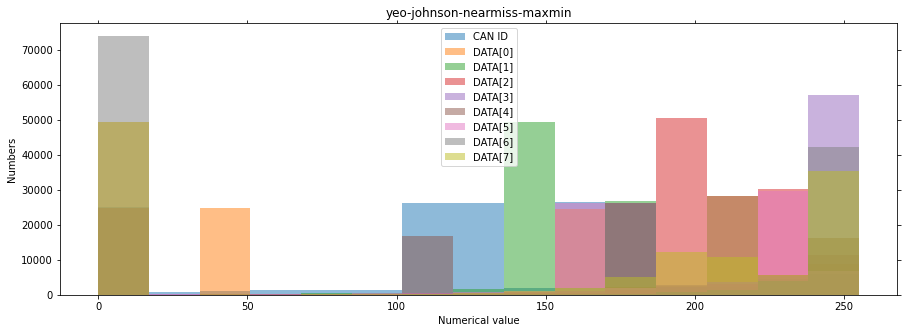
\includegraphics[width=1 \textwidth]{figures/yeo-johnson-nearmiss-maxmin.png}
        \end{minipage}
    }
    \subfigure[QuantileTransformer-normal-nearmiss-maxmin]{
        \begin{minipage}[b]{1\linewidth}
        \centering
        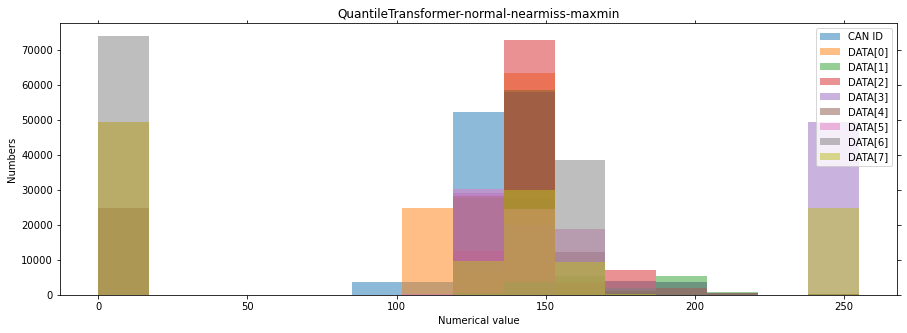
\includegraphics[width=1 \textwidth]{figures/QuantileTransformer-normal-nearmiss-maxmin.png}
        \end{minipage}
    }
    \caption{Two kinds of histograms after power transformation}
     \label{fig:Two kinds of histograms after power transformation}
\end{figure}

\subsection{实验结果与分析}\label{subsection:Generating_images}

\textbf{数据图像化的方法和效果。}\label{subsection:Data_imageization}为了适应CNN类模型的输入要求,本节将原始的文本类数据转化为图像数据。本节参考了文献\cite{A_Transfer_Learning_and_Optimized_CNN_Based_Intrusion_Detection_System_for_Internet_of_Vehicles}中的处理方案,将Car-Hacking数据集中的每条记录按照其9个特征值分别映射到一个3x3的灰度像素块上,然后将9个像素块拼接成一个9x9的大像素块。为了增加图像的信息量和多样性,本节将三个不同的9x9像素块叠加在一起,形成一个9x9的彩色图像。图\ref{fig:five picture after yeo and qtn}展示了两种不同的幂转化方法生成的图像示例。为了方便后续的CNN模型处理,本节对生成的图像进行了reshape操作,将其大小调整为224x224。

\begin{figure}[htb]
    \centering
    \subfigure[yeo-johnson-nearmiss-maxmin]{
        \begin{minipage}[b]{1\linewidth}
            \centering
            \includegraphics[width=0.9 \textwidth]{figures/yeo-johnson.png}
        \end{minipage}
    }
    \subfigure[QuantileTransformer-normal-nearmiss-maxmin]{
        \begin{minipage}[b]{1\linewidth}
            \centering
            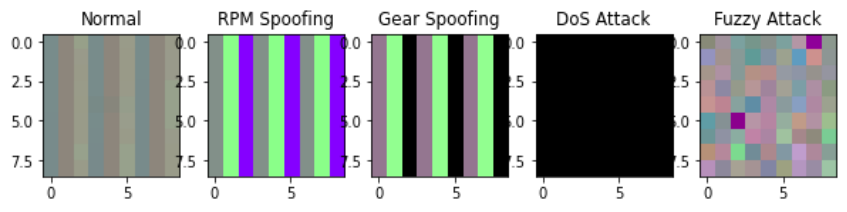
\includegraphics[width=0.9 \textwidth]{figures/quantile Transformer.png}
        \end{minipage}
    }
    \caption{Five kinds of pictures after two kinds of power transformation}
    \label{fig:five picture after yeo and qtn}
\end{figure}

\textbf{数据集划分和模型训练。}\label{subsection:Dataset_split_and_model_training}本节将生成的4395张图像数据按照8:2的比例划分为训练集和测试集,然后使用pysyft库实现联邦平均算法,定义了两个虚拟的参与者,并将训练集平均分配给他们。本节选择了一个自定义的CNN模型作为基准模型,由两个卷积层、一个最大池化层、一个平均池化层和一个全连接层组成,激活函数采用了Relu函数。使用SGD作为优化器,交叉熵作为损失函数,设置了epoch为50,Batch Size为128。图\ref{fig:FL_CNN}展示了使用yeo-Johnson幂转化和quantile Transformer幂转化后的数据进行训练的结果,可以看出,yeo-Johnson幂转化后的数据在损失函数和准确率上都有更快的收敛速度,说明本节提出的yeo-Johnson幂转化方法是有效的。

\begin{figure}[htb]
    \centering
    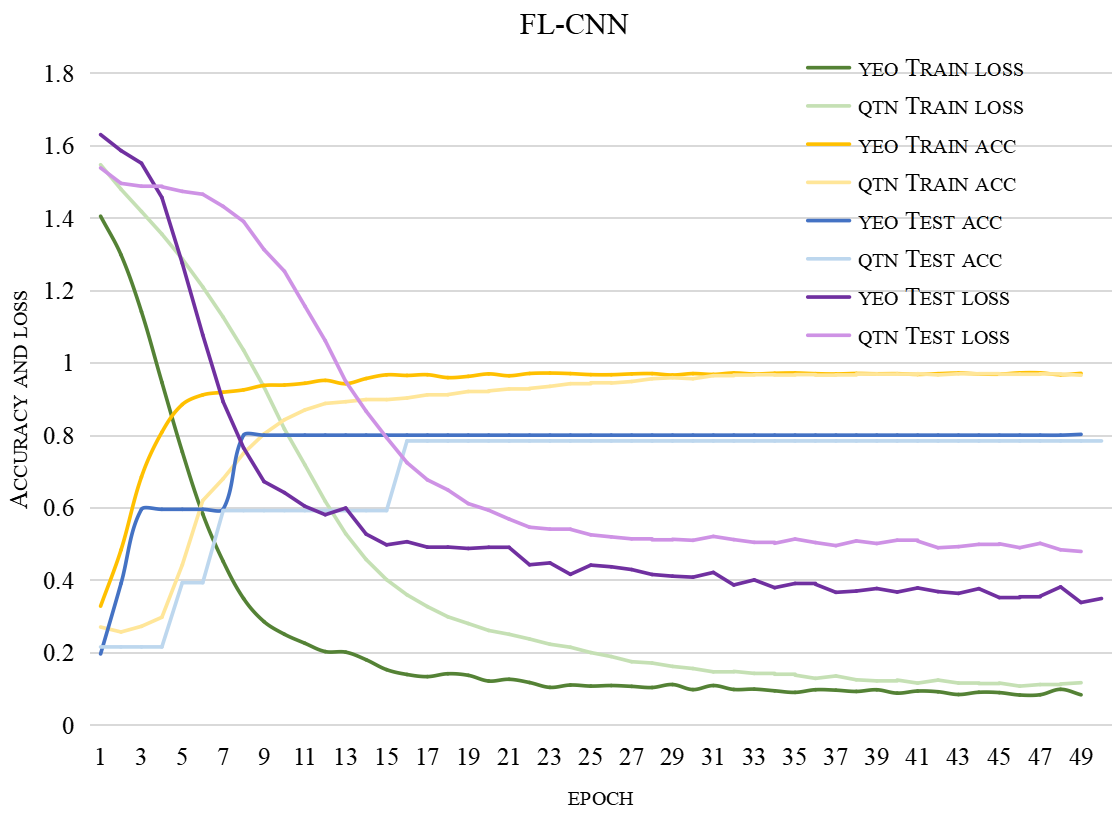
\includegraphics[width=0.45 \textwidth]{figures/FL_CNN.png}
    \caption{QuantileTransformer-normal-nearmiss-maxmin}
    \label{fig:FL_CNN}
\end{figure}

\textbf{分类结果的评估。}\label{subsection:Classification_result_evaluation}为了评估不同的CNN模型在分类任务上的性能,本节绘制了每个模型的混淆矩阵。混淆矩阵是一种常用的评价分类模型的指标,它可以在数据不平衡的情况下,直观地显示模型对每个类别的预测准确率。混淆矩阵的列代表预测的类别,行代表真实的类别。对角线上的元素表示预测正确的数量或比例,非对角线上的元素表示预测错误的数量或比例。本节期望得到的混淆矩阵是对角线上的值越大越好,表示模型能够正确地区分不同的类别。图\ref{fig:Confusion matrix of 4 types of models}显示了四种CNN模型的混淆矩阵,从中可以发现,除了ResNet18以外,其他的模型都能够较好地识别出少数类,即异常流量,只有少量的正常流量被误判为异常流量,这种情况是可以接受的,因为将异常流量误判为正常流量会带来更大的风险。ResNet18则能够完美地识别出正常流量,但是对异常流量的识别能力较差,因此本节保留了它,以备在特殊场景中使用。

\begin{figure}[htb]
\centering    
    \subfigure{
        \begin{minipage}[b]{.4\linewidth}
            \centering
            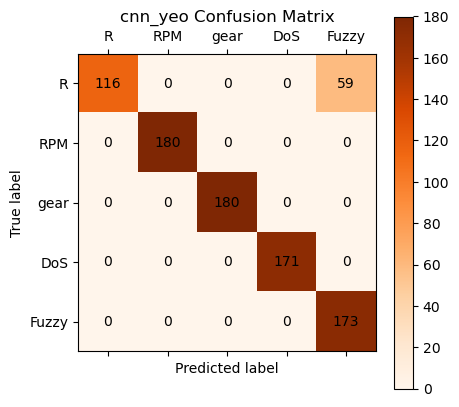
\includegraphics[scale=0.35]{figures/cnn_yeo_Confusion_Matrix.png}
            % \caption{FL-vgg16 Confusion Matrix}
        \end{minipage}
    }
    \subfigure{
        \begin{minipage}[b]{.4\linewidth}
            \centering
            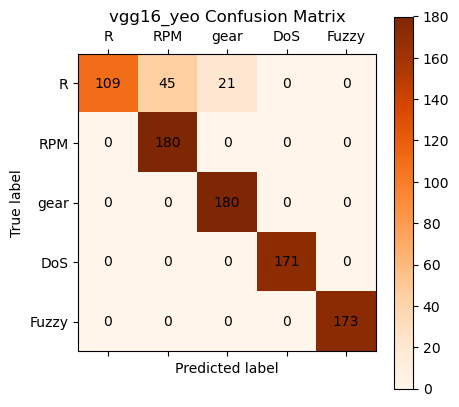
\includegraphics[scale=0.35]{figures/vgg16_yeo_Confusion_Matrix.png}
            % \caption{FL-vgg16 Confusion Matrix}
        \end{minipage}
    }

    \subfigure{
        \begin{minipage}[b]{.4\linewidth}
            \centering
            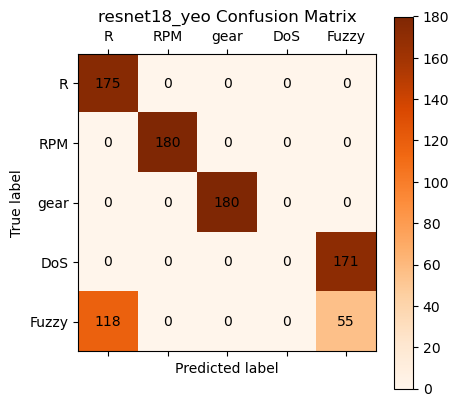
\includegraphics[scale=0.35]{figures/resnet18_yeo_Confusion_Matrix.png}
            % \caption{FL-vgg16 Confusion Matrix}
        \end{minipage}
    }
    \subfigure{
        \begin{minipage}[b]{.4\linewidth}
            \centering
            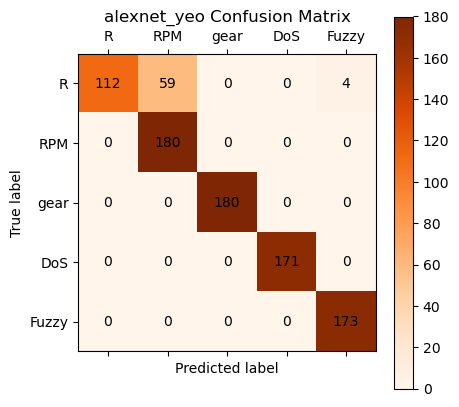
\includegraphics[scale=0.35]{figures/alexnet_yeo_Confusion_Matrix.png}
            % \caption{FL-vgg16 Confusion Matrix}
        \end{minipage}
    }
    \caption{Confusion matrix of 4 types of models}
    \label{fig:Confusion matrix of 4 types of models}
\end{figure}

\textbf{ROC曲线和AUC值的比较。}\label{subsection:ROC_curve_and_AUC_value_comparison}为了评估不同的FL模型在分类任务上的灵敏度和特异度,本节绘制了四种FL模型的ROC曲线,并计算了它们的AUC值。ROC曲线是一种用于评价二分类模型的性能的图形工具,它反映了模型的真阳性率(TPR)和假阳性率(FPR)之间的关系。AUC值是ROC曲线下的面积,它表示模型对正负样本的区分能力,其值越接近1,表示模型的性能越好。图\ref{fig:ROC curve and AUC area of five types of models}显示了四种FL模型的ROC曲线和AUC值,从中可以看出,CNN、VGG16、AlexNet模型的AUC值都达到了1,说明它们能够完美地区分正负样本,而ResNet18模型的AUC值也高达0.94,表明它也有很高的分类性能。因此,本节认为这四种FL模型都能够胜任日常的入侵检测工作。

\begin{figure}[htb]
\centering    
    \subfigure{
        \begin{minipage}[b]{.4\linewidth}
        \flushleft
        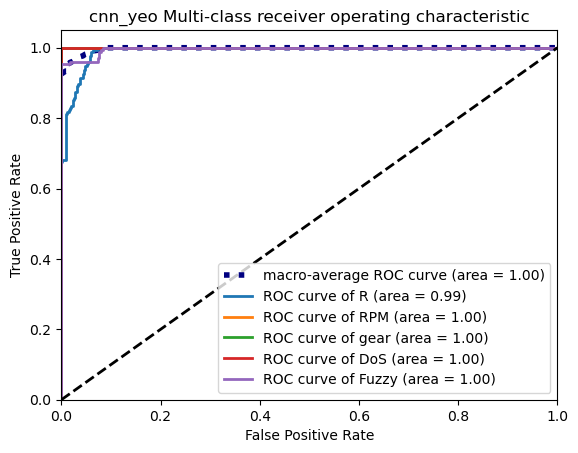
\includegraphics[scale=0.26]{figures/cnn_yeo_roc_fig.png}
        % \caption{FL-vgg16 Confusion Matrix}
        \end{minipage}
    }
    \subfigure{
        \begin{minipage}[b]{.4\linewidth}
            \flushright
            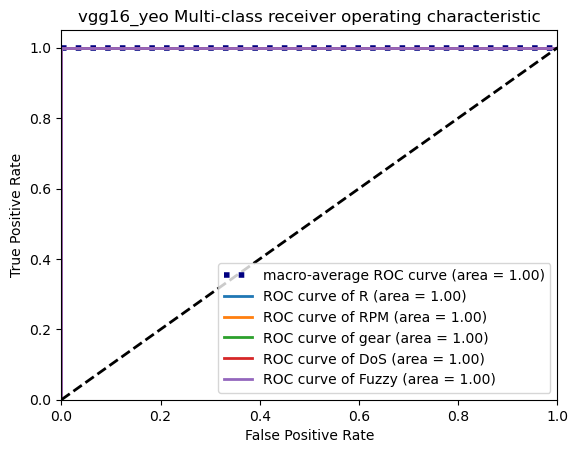
\includegraphics[scale=0.26]{figures/vgg16_yeo_roc_fig.png}
            % \caption{FL-vgg16 Confusion Matrix}
        \end{minipage}
    }

    \subfigure{
    \begin{minipage}[b]{.4\linewidth}
        \flushleft
        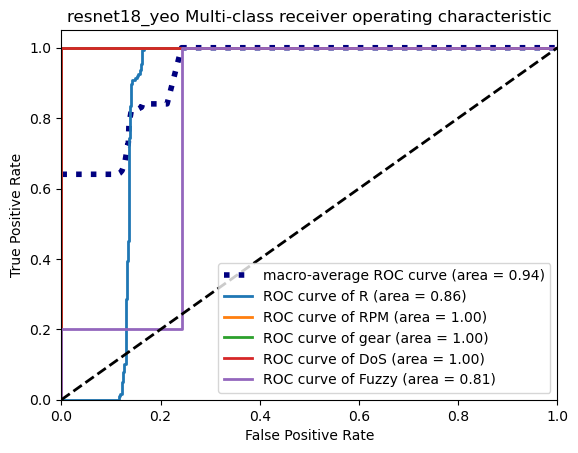
\includegraphics[scale=0.26]{figures/resnet18_yeo_roc_fig.png}
        % \caption{FL-vgg16 Confusion Matrix}
    \end{minipage}
    }
    \subfigure{
        \begin{minipage}[b]{.4\linewidth}
            \flushright
            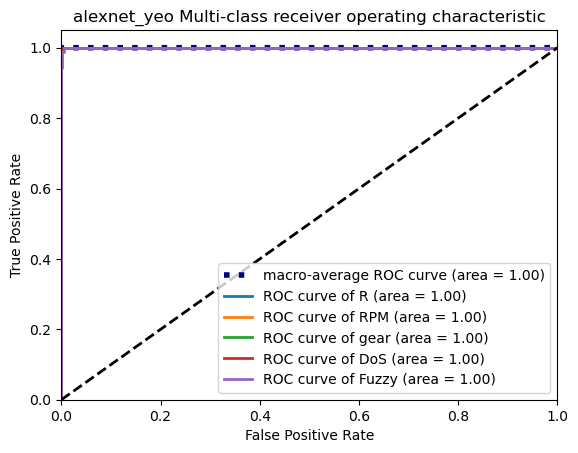
\includegraphics[scale=0.26]{figures/alexnet_yeo_roc_fig.png}
            % \caption{FL-vgg16 Confusion Matrix}
        \end{minipage}
    }
    \caption{ROC curve and AUC area of five types of models}
    \label{fig:ROC curve and AUC area of five types of models}
\end{figure}

\textbf{模型对比情况的统计分析。}\label{subsection:Model_comparison_statistics}本节对FL-CNN、FL-VGG16、FL-ResNet18、FL-AlexNet四种FL模型的性能进行了统计分析,结果如表\ref{table:Four federated learning models}所示。从表中可以看出,FL-AlexNet模型在达到最佳状态时的epoch数最少,只有10次,而其他模型都需要20次或以上。这说明FL-AlexNet模型的收敛速度较快,能够在较少的迭代次数下达到较高的准确率。另一方面,FL-CNN模型的平均训练时间最短,只有473.13秒,而FL-VGG16模型的平均训练时间最长,为712.26秒。这表明FL-CNN模型的计算效率较高,而FL-VGG16模型的计算效率较低。然而,考虑到FL模型的训练时间主要取决于参与者的网络状况和设备性能,而不是模型本身的复杂度,因此这些训练时间的差异并不显著,都在可以接受的范围内。

\begin{table}[htbp]
    \centering
    \caption{Four federated learning models}
    \begin{tabular}{ccccc}
    \hline
        \textbf{} & \textbf{FL-CNN} & \textbf{FL-VGG16} & \textbf{FL-ResNet18} & \textbf{FL-AlexNet} \\ \hline
        \text{$t_t$(s)} & 82.242301 & 713.2586751 & 244.2694107 & 146.4923077 \\ 
        \text{Best Epoch} & 9 & 3 & 34 & 5 \\ 
        \text{Size(KB)} & 222 & 524,541 & 43,725 & 222,754 \\ 
        \text{精度} & 0.932878271 & 0.924914676 & 0.671217292 & 0.928327645 \\ 
        \text{查准率P} & 0.949137931 & 0.939104478 & 0.568126491 & 0.946107841 \\ 
        \text{召回率} & 0.932571429 & 0.924571429 & 0.663583815 & 0.928 \\ 
        \text{F1 Score} & 0.930314369 & 0.920275282 & 0.604710494 & 0.925649556 \\ 
        \text{Roc\_auc R} & 0.991347403 & 1 & 0.864147727 & 1 \\ 
        \text{Roc\_auc RPM} & 1 & 1 & 1 & 1 \\ 
        \text{Roc\_auc Gear} & 1 & 1 & 1 & 1 \\ 
        \text{Roc\_auc Dos} & 1 & 1 & 1 & 1 \\ 
        \text{Roc\_auc Fuzzy} & 0.996782328 & 1 & 0.806792317 & 0.999885376 \\ \hline
    \end{tabular}
    \label{table:Four federated learning models}
\end{table}

\section{本章小结}

本章介绍了一种基于迁移学习和特征工程的联邦学习CAN异常检测设计框架。MEC作为边缘计算平台,负责对来自不同RSU的联邦模型进行聚合更新和数据存储。RSU作为车联网的核心节点,负责本地模型的训练、数据收集、清洗和异常检测执行,并将检测结果反馈给所属区域的车辆。RSU根据车辆识别码(VIN)对区域内的车辆进行K-means聚类,从每个类别中选择$k \geq 1$辆车作为本地数据来源。为了在智能车上实现入侵检测,本章采用了轻量级的DL模型和欠采样技术,以降低计算资源消耗并解决样本不均衡的问题。此外,引入了特征工程思想,对数据进行了非线性变换(yeo-Johnson变换),然后使用min-max标准化将数据缩放到$0-1$之间。迁移学习的思想也被引入,利用多个领域的共享知识来建立有效的模型。MEC中集成四类预训练后的DL模型,分别是CNN、VGG16、ResNet18和AlexNet。在系统启动的初期,MEC会将这四类模型下发给选中的$\alpha$个RSUs。最后,研究了在移动边缘计算(MEC)环境下,如何为不同类型的路侧单元(RSU)提供个性化的深度学习(DL)模型,以实现车辆入侵检测的联邦学习任务。MEC作为系统的中心节点,负责模型的聚合与分发。整个系统将一直重复这个过程,直到$g_{t+1}$收敛。MEC将持续监控达到收敛状态的全局模型,一旦发现由于车辆移动导致的RSU收集到的CAN数据变化、特殊RSU离线等原因导致模型检测性能下降,将再次重启整个联邦学习过程。

% 随着智能车辆的功能越来越多,其暴露出来的脆弱点也在增多。当这些暴露出来的脆弱面被攻击者恶意利用时,会给用户及企业带来隐私泄露、功能故障、财产损失甚至生命威胁。本节发现车联网中存在的安全问题具有高度的动态性、复杂性和隐蔽性等特点。针对动态性,本节提出将IDS的主动权交给静态的RSU,而不断移动的车辆为被检测者,本节提出将CP-ABE加密策略应用于RSU与车之间的数据交换,在保障网络交换效率的同时兼顾了数据信息安全。针对车联网攻击的复杂性和隐蔽性,本节提出迁移学习结合联邦学习技术进行入侵检测。接下来本节将从车联网外攻击扩展到车联网内外的攻击,以此来探究本节提出的模型是否具有普适性。 								%第三章
	\setlength{\baselineskip}{20pt}
\chapter{基于稀疏学习和梯度扰动的梯度泄露防护}
\label{cha:chap4}

上一章提出了一个联邦学习系统,旨在保护车联网中的数据隐私。然而,本文的关注点不仅仅在于联邦学习的应用,更着重于联邦学习本身。现有研究表明,原始的联邦学习并非绝对安全,攻击者可以根据泄露的梯度数据推导出原始的训练数据。因此,本章将进一步研究保护数据隐私的方法,以防止敌手从共享的梯度中重构出敏感的训练样本。为此,本章提出了一个基于稀疏学习和梯度扰动的梯度泄露防护方案。该方案的核心思想分为两部分。首先,利用系数学习方法将训练数据表示为稀疏字典学习(DL)的形式,从而降低数据的可识别性。其次,为了进一步增强模型的鲁棒性,对全连接(FC)层的梯度进行了随机扰动,以抵抗梯度泄露的攻击。最后,本章在不同的数据集和攻击场景下进行了实验,最终验证了所提出方法的有效性和优越性。这种防御方法可以与现有的联邦学习系统结合,而无需修改训练协议。通过广泛的实验,还证明了所提出的方法可以有效地抵抗重构攻击,同时具有高效性和可忽略的性能损失。

\section{相关工作和技术介绍}

\subsection{特征提取与稀疏学习}

在机器学习中,数据的属性通常称为“特征”(feature),与当前学习任务有关的属性称为“相关特征”(relevant feature),与当前学习任务无关的属性称为“无关特征" (irrelevant feature)。从给定的特征集合中选择出一个相关特征的子集,这个过程称为 “特征选择"(feature selection)。特征选择是“数据预处理”(data preprocessing)的一个重要步骤,在实际的机器学习任务中,通常需要先对数据进行特征选择,然后再用选出的特征来训练学习器。特征选择的目的有两个:一是为了缓解“维数灾难”(curse of dimensionality)问题,这是由于特征过多导致的。如果能够从众多的特征中挑选出最重要的特征,那么后续的学习过程就可以只在这些特征上建立模型,从而降低维度,减少计算和存储的开销,提高模型的可解释性。二是为了降低学习任务的难度,因为去除无关特征可以消除数据中的噪声和冗余,提高数据的质量,从而提高学习器的性能。特征选择过程要注意不要丢失重要特征,否则会导致信息的损失,影响学习器的泛化能力。有些特征虽然包含的信息可以从其他特征中推导出来,但是它们并不是无用的,这些特征称为“冗余特征"(redundant feature)。冗余特征在某些情况下是有益的,比如当它们恰好对应了学习任务所需的“中间概念”时,它们可以降低学习任务的难度。特征选择方法通常由两个部分组成:特征子集的搜索机制和特征子集的评价机制。根据这两个部分的不同,特征选择方法可以分为三类:过滤式(filter)、包裹式(wrapper)和嵌入式(embedding)。

把数据集$D$看作一个矩阵,其中每一行代表一个样本,每一列代表一个特征。特征选择要解决的问题是特征的“稀疏性”,即矩阵中的许多列与当前的学习任务无关,如果能够通过特征选择去掉这些列,那么学习器的训练过程就只需要在一个较小的矩阵上进行,这样可以降低学习任务的难度,减少计算和存储的开销,提高模型的可解释性。另一种稀疏性是指矩阵中存在很多零元素,但这些零元素并不是以整列或整行的形式出现的,而是分散在矩阵中的不同位置。这种稀疏性对学习任务来说是有利的,比如线性支持向量机在文本数据上的表现就很好,这是因为文本数据在使用字频表示后具有很高的稀疏性,使得大多数问题变得线性可分。同时,这种稀疏性也不会造成存储上的负担,因为稀疏矩阵有很多高效的存储方法。

“字典学习”(dictionary learning)或者“稀疏编码”(sparse coding)则是其中一种将样本转换为字典中的线性组合的方法,它们能够赋予密集表示的样本稀疏性,从而简化学习任务,降低模型的复杂度。给定数据集$\boldsymbol{x}_1, \boldsymbol{x}_2, \ldots, \boldsymbol{x}_m$,字典学习的最简单形式可以表示为以下优化问题:
\begin{equation}
\min_{\mathbf{B},\boldsymbol{\omega}_i}\sum_{i=1}^m\|\boldsymbol{x}_i-\mathbf{B}\boldsymbol{\omega}_i\|_2^2+\lambda\sum_{i=1}^m\|\boldsymbol{\omega}_i\|_1\:,
\label{eq:dictionary_learning}
\end{equation}
其中$\mathbf{B} \in \mathbb{R}^{d \times k}$是字典矩阵,$k$是字典的词汇量,通常由用户指定。$\boldsymbol{\omega}_i \in \mathbb{R}^k$表示样本$\boldsymbol{x}_i \in \mathbb{R}^d$的稀疏表示。式\ref{eq:dictionary_learning}中的第一项旨在使$\boldsymbol{\omega}_i$能够尽可能地重构$\boldsymbol{x}_i$,而第二项则旨在使$\boldsymbol{\omega}_i$尽可能地稀疏。

为了求解式\ref{eq:dictionary_learning},可以采用变量交替优化的策略。首先,固定字典$\mathbf{B}$,优化$\boldsymbol{\omega}_i$。这时,可以将式\ref{eq:dictionary_learning}按分量展开,发现其中没有涉及到$\omega_i^u \omega_i^v$($u \neq v$)这样的交叉项。因此,可以参考LASSO的解法,求解以下问题,从而得到每个样本$\boldsymbol{x}_i$的稀疏表示$\boldsymbol{\omega}_i$:

\begin{equation}
\min_{\boldsymbol{\omega}_i}\|\boldsymbol{x}_i-\mathbf{B}\omega_i\|_2^2+\lambda\|\boldsymbol{\omega}_i\|_1\:.
\label{eq:dictionary_learning_3}
\end{equation}

接下来,固定$\boldsymbol{\omega}_i$,优化字典$\mathbf{B}$。这时,可以将式\ref{eq:dictionary_learning}写为以下形式:

\begin{equation}
\min_{\mathbf{B}}\|\mathbf{X}-\mathbf{BA}\|_{F}^{2},
\label{eq:dictionary_learning_4}
\end{equation}

其中$\mathbf{X} = (\boldsymbol{x}_1, \boldsymbol{x}_2, \ldots, \boldsymbol{x}_m) \in \mathbb{R}^{d \times m}$,$\mathbf{A} = (\boldsymbol{\omega}_1, \boldsymbol{\omega}_2, \ldots, \boldsymbol{\omega}_m) \in \mathbb{R}^{k \times m}$,$\|\cdot\|_F$表示矩阵的Frobenius范数。式\ref{eq:dictionary_learning_4}有多种求解方法,其中一种常用的方法是基于逐列更新策略的KSVD。令$b_i$表示字典矩阵$B$的第$i$列,$\omega_i$表示稀疏矩阵$A$的第$i$行,式\ref{eq:dictionary_learning_4}可重写为:

\begin{equation}\begin{aligned}
\operatorname*{min}_{\mathbf{B}}\|\mathbf{X}-\mathbf{BA}\|_{F}^{2}& =\min_{\boldsymbol{b}_{i}}\left\|\mathbf{X}-\sum_{j=1}^{k}\boldsymbol{b}_{j}\boldsymbol{\omega}^{j}\right\|_{F}^{2}  \\
&=\min_{\boldsymbol{b}_i}\left\|\left(\mathbf{X}-\sum_{j\neq i}\boldsymbol{b}_j\boldsymbol{\omega}^j\right)-\boldsymbol{b}_i\boldsymbol{\omega}^i\right\|_F^2 \\
&=\min_{\boldsymbol{b}_{i}}\left\|\mathbf{E}_{i}-\boldsymbol{b}_{i}\boldsymbol{\omega}^{i}\right\|_{F}^{2}\:.
\end{aligned}
\label{eq:dictionay_learning 4}
\end{equation}

在更新字典的第$i$列时,其他各列都保持固定。因此,有$\mathbf{E}_i=\sum_{j\neq i}\boldsymbol{b}_j\boldsymbol{\omega}^j$是一个固定项。为避免直接对$\mathbf{E}_i$进行奇异值分解而破坏稀疏性,KSVD算法对$\mathbf{E}_i$和$\omega_i$进行特殊处理:$\omega_i$仅保留非零元素,$\mathbf{E}_i$则仅保留与$\boldsymbol{b}_i$和$\boldsymbol{\omega}^i$的非零元素相乘的项,然后再进行奇异值分解,以保持第一步得到的稀疏性。通过对字典矩阵$B$进行初始化,然后反复迭代上述两步,最终就可以得到字典$B$和样本$x_i$的稀疏表示$\omega_i$。在字典学习的过程中,用户可以通过设置字典的词汇量$k$来控制字典的规模,从而影响稀疏表示的程度。

% 有时间把K-SVD扩充一下:https://blog.csdn.net/qq_37085158/article/details/122559053 https://ieeexplore.ieee.org/document/1710377

\subsection{差分隐私}

如图\ref{fig:three major privacy guarantees}所示,数据隐私技术涵盖了多个方面,包括模糊技术、扰动技术、加密技术、混合隐私技术、分布式计算框架和区块链技术。其中,扰动技术专注于对数据本身进行扰动,主要体现在差分隐私技术上。差分隐私通过在数据上直接添加随机噪声,或者将原始值以一定概率扰动为随机值,从而实现隐私保护。与传统的统计披露限制方法(如k-匿名)不同,差分隐私能够抵御具有任意背景知识和计算能力的攻击,并最大限度地延缓因多次发布而造成的隐私泄露风险。此外,差分隐私不依赖算法和参数的保密性,且任何计算都无法削弱已有的隐私保障。由于严格的数学保证和良好的隐私性质,差分隐私已被谷歌、苹果、微软、脸书、领英及美国人口普查局等机构采纳,并在生产系统中用于保护参与者的隐私。

\begin{figure}[htb]
\centering
    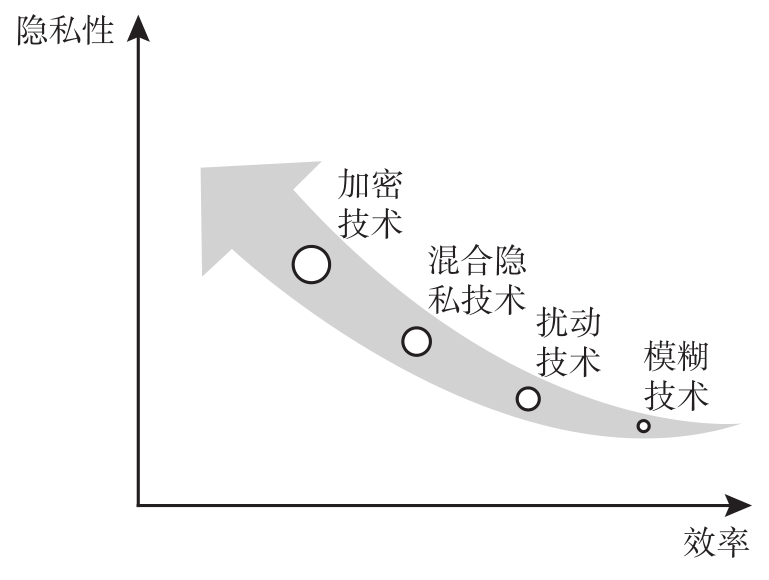
\includegraphics[scale=1.5]{figures/chapter4/Comparison of privacy and efficiency of different privacy technologies.jpg}
    % \caption{FL-vgg16 Confusion Matrix}
    \caption{不同隐私技术在隐私性与效率上的对比}
    \label{fig:three major privacy guarantees}
\end{figure}

然而,通过扰动保护数据隐私会导致数据可用性降低,从而影响计算结果的准确性。因此,在保护数据隐私的前提下,如何尽可能提高扰动对数据可用性的影响,成为该技术的核心问题。通常,满足差分隐私的算法有两种数据扰动方式:一种是直接在计算结果上添加噪声,常用的包括拉普拉斯机制、指数机制等;另一种是以一定的概率对数据进行扰动,即随机响应机制。在定义差分隐私之前,首先定义两个数据库之间的距离。

数据库距离定义。将数据库$x$的$L_1$范数记作$\parallel x\parallel_1=\sum_{i=1}^{| x|}\parallel x\parallel_i$,则两个数据库之间的$L_1$距离便是$\parallel x-y\parallel_1$。若将$\parallel x\parallel_1$作为数据库$x$大小的度量,即$x$中一共包含几行记录,则$\parallel x-y\parallel_1$便用于度量数据库$x$和$y$中有几行不同的记录,也就是数据库之间的距离。

差分隐私定义。对于一个随机算法$\mathcal{M}$,其值域为$Range(\mathcal{M})$,如果对$Range(\mathcal{M})$的任意子集$S$和$\mathcal{M}$定义域上的一对相邻数据集$x$和$y$($\parallel x - y \parallel_1 \le 1$),有$\Pr[\mathcal{M}(x)\in S]\leq e^{\varepsilon}Pr[\mathcal{M}(y)\in S]+\delta$,则称算法$M$满足$(\varepsilon ,\delta)$-差分隐私。其中,$\Pr[\mathcal{M}(x)\in S]$表示在输入为$x$时,机制$\mathcal{M}$的输出落在集合$S$中的概率。这里,$\mathcal{M}$是一个隐私保护机制,例如一个加噪声的查询回答器。$\Pr[\mathcal{M}(y)\in S]$表示输入为$y$时,同样的机制$\mathcal{M}$的输出落在集合$S$中的概率。注意,$x$和$y$是相邻的输入,即它们在数据上非常接近。$e^{\varepsilon}$是一个指数项,用于衡量输入$x$和$y$之间的相似性,表示在隐私保护机制中,输出在$x$和$y$之间的概率差异。$\delta$是一个小常数(通常接近零),表示额外的隐私参数,当$\delta=0$时,则说算法$M$满足$\varepsilon $-差分隐私。这个不等式表明:如果一个机制$\mathcal{M}$是差分隐私的,那么在输入$x$和$y$之间的输出概率不会有显著的差异。也就是说,$\mathcal{M}$确保了相似输入的输出概率“接近”,同时允许一小部分额外的隐私损失(由$\delta$控制)。可以看到,当$\varepsilon $越小意味着,攻击者越难区分这对相邻数据集,保护程度越高。反之,当$\varepsilon $越大时,保护程度就越低。一般情况下,也把$\varepsilon $叫作隐私预算。

\begin{figure}[htb]
\centering
    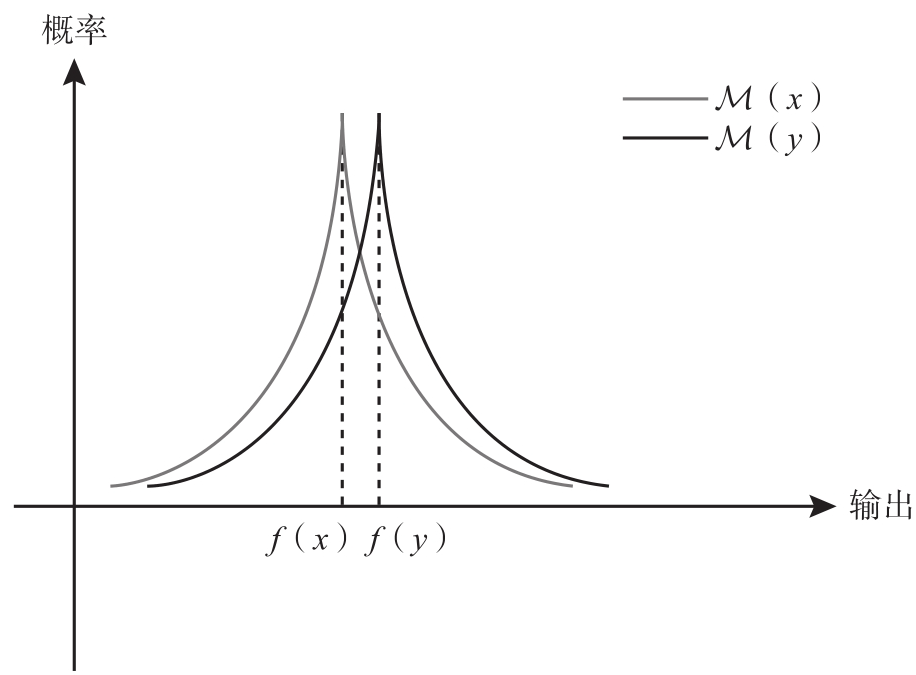
\includegraphics[scale=1]{figures/chapter4/dp figure.png}
    % \caption{FL-vgg16 Confusion Matrix}
    \caption{差分隐私算法在邻近数据集上的输出概率}
    \label{fig:dp figure}
\end{figure}

函数敏感度。对于一个查询函数$f(·)$,它作用于一对相邻数据集$x$和$x′$,返回结果的最大变化范围,便是该查询函数的函数敏感度:
\begin{equation}\mathrm{Sensitivity}(f)=\max_{x,x^{\prime}}\parallel f(x)-f(x^{\prime})\parallel_{1}
\end{equation}
需要注意的是,函数敏感度只由查询函数本身决定,与查询的数据集无关。

拉普拉斯差分隐私。对于连续型数据的查询结果,拉普拉斯机制在查询结果上加入一个满足分布$\text{Lap}\bigg(0,\frac{\text{Sensitivity}(f)^{\odot}}{\varepsilon}\bigg)$的噪声,来实现差分隐私。其中$Sensitivity(f)$为查询函数敏感度,$\varepsilon$为隐私预算。以$x$表示被查询的数据库,$M(x)$表示最后的查询结果,$f(x)$表示原先查询函数返回的查询结果,$Y$表示满足拉普拉斯分布的噪声,即$Y\thicksim\text{Lap}\bigg(0,\frac{\text{Sensitivity}(f)}{\varepsilon}\bigg)$,则拉普拉斯机制可以表示为$M(x)=f(x)+Y$。

拉普拉斯机制满足$\varepsilon$-差分隐私。根据这一定义,可以看到隐私预算越小、扰动越大,则结果的可用性越小,隐私保护程度越高。下面将证明拉普拉斯机制满足$\varepsilon $-差分隐私。假设$x$和$y$为两个相邻数据集,即$\parallel x - y \parallel_1 \le 1$,而$f$表示未加噪的查询函数返回的结果,$M(x)$表示最后查询函数返回的结果,$p_x$为$M(x)$的概率密度函数,$p_y$为$M(y)$的概率密度函数。比较位于$f$值域中的任意一点$z$,有

\begin{equation}
\begin{aligned}
\frac{p_x(z)}{p_y(z)} &= \prod_{i=1}^{k} \frac{\exp\left(\frac{e|f(x)_i - z_i|}{\Delta f}\right)}{\exp\left(\frac{e|f(y)_i - z_i|}{\Delta f}\right)} \\
&= \prod_{i=1}^{k} \exp\left(\frac{e(|f(y)_i - z_i| - |f(x)_i - z_i|)}{\Delta f}\right) \\
& \leq \prod_{i=1}^{k} \exp\left(\frac{e(|f(x)_i - f(y)_i|)}{\Delta f}\right) \\
&= \exp\left(\frac{e \cdot ||f(x) - f(y)||_1 }{ {\Delta f}}\right)
\leq \exp(e)
\end{aligned}
\end{equation}

上式第一个不等式可根据三角不等式得出,最后一个不等式则根据函数敏感度定义和$\parallel x - y \parallel_1 \le 1$得出。对称地,我们有[插图]。证毕。

差分隐私会不可避免地引入统计噪声。隐私保护需要随机性,不平凡(最少有两种不同输出)的确定算法无法满足差分隐私,如图8.3所示。对于不平凡的确定算法,一定存在两个仅相差一条记录的数据集(如红色和绿色的正方形)被同一函数映射到不同结果(如红色和绿色的三角形)的情况,这将使攻击者明确这条记录的存在或缺失,从而泄露应答者的隐私。尽管差分隐私算法具有相当大的灵活性,但不确定性的增加必然会造成统计效用的损失。一种简单的办法是不断提升样本容量,从而使差分隐私噪声所造成的误差远小于系统的固有误差(如抽样误差)。如何缓解统计隐私和效用的紧张关系是差分隐私研究的核心问题。

差分隐私不依赖算法和参数的保密性。柯克霍夫(Kerckhof)原则告诉我们,密码系统的安全不应依赖除密钥以外任何事物的保密性,这无疑与仰仗算法保密的模糊式安全(security by obscurity)形成了鲜明对比。在差分隐私之前,统计披露控制大多以黑箱形式进行。统计机构需要隐藏数据的变换程度,从而保留数据用户对分析结果的不确定性。差分隐私继承了Kerckhof原则,只有随机种子需要保密,而隐私算法和参数的公开并不影响其所提供的隐私保证。这种透明性首次将隐私与效用的权衡取舍置于众目之下,既能帮助政策制定者做出科学、合理的决策,也能强化人们对所用隐私技术的理解、信任与监督

\begin{figure}[htb]
\centering
    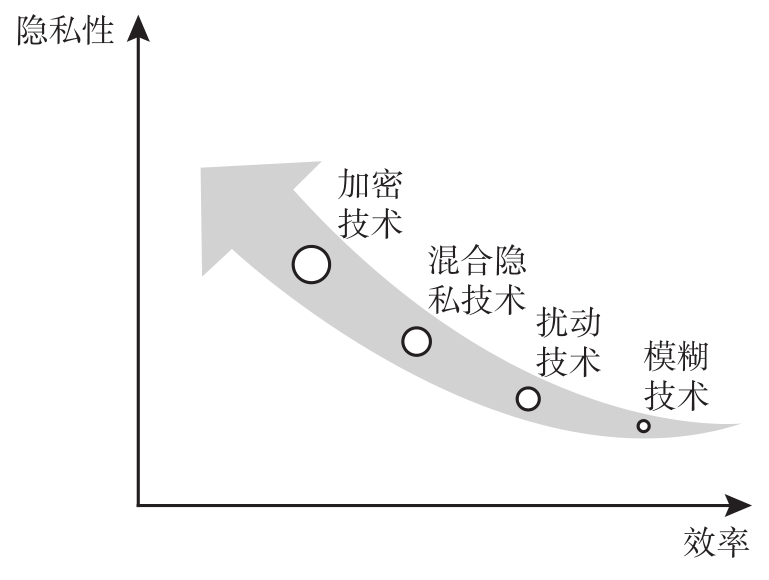
\includegraphics[scale=0.5]{figures/chapter4/Comparison of privacy and efficiency of different privacy technologies.jpg}
    % \caption{FL-vgg16 Confusion Matrix}
    \caption{不同隐私技术在隐私性与效率上的对比}
    \label{fig:Cluster the cars in the region}
\end{figure}

差分隐私用于隐私保护时,需要处理的数据可以分为两大类——连续型数据和离散型数据。连续型数据往往是一个连续区间内的数值取值,如树的高度、房屋的宽度等;离散型数据则可以对数据进行一一列举,如彩虹的七种颜色、人的五根手指等。差分隐私的主要思想是对数据添加扰动,而对于不同类型的数据,扰动的类型也不相同。对连续型数据,常用的扰动机制是拉普拉斯机制。对离散型数据,常用的是指数机制。拉普拉斯机制在介绍拉普拉斯机制前,需要先介绍一下敏感度。差分隐私通过对数据添加扰动(加噪)来保护用户隐私,如果扰动过大,则会导致数据可用性太差影响数据使用,如果扰动过小,则可能会导致用户隐私被攻击者获取、保护能力下降。由此可见,扰动的大小是差分隐私中一个重要的量,敏感度便是用于控制扰动大小的参数。定义4.3 函数敏感度.对于一个查询函数f(·),它作用于一对相邻数据集x和x′,返回结果的最大变化范围,便是该查询函数的函数敏感度

\begin{equation}
\mathrm{Sensitivity}(f)=\max_{x,x^{\prime}}\parallel f(x)-f(x^{\prime})\parallel_{1}
\end{equation}

需要注意的是,函数敏感度只由查询函数本身决定,与查询的数据集无关。有了函数敏感度的定义后,接下来介绍拉普拉斯机制。对于连续型数据的查询结果,拉普拉斯机制在查询结果上加入一个满足分布$\begin{aligned}\text{Lap}\bigg(0,&\frac{\text{Sensitivity}(f)^{\odot}}{\varepsilon}\bigg)\end{aligned}$的噪声,来实现差分隐私。其中Sensitivity(f)为查询函数敏感度,$\varepsilon$ 为隐私预算。

定义4.4 拉普拉斯机制.以$x$表示被查询的数据库,$M(x)$表示最后的查询结果,$f(x)$表示原先查询函数返回的查询结果,$Y$表示满足拉普拉斯分布的噪声,即$\begin{aligned}Y&\thicksim\text{Lap}\bigg(0,\frac{\text{Sensitivity}(f)}{\varepsilon}\bigg)\end{aligned}$,则拉普拉斯机制可以表示为$M(x)=f(x)+Y$

拉普拉斯机制满足$\varepsilon $-差分隐私。根据这一定义,可以看到隐私预算越小、扰动越大,则结果的可用性越小,隐私保护程度越高。下面将证明拉普拉斯机制满足$\varepsilon $-差分隐私。假设$x$和$y$为两个相邻数据集,即$\parallel x - y \parallel_1 \le 1$,而f表示未加噪的查询函数返回的结果,$M(x)$表示最后查询函数返回的结果,$p_x$为$M(x)$的概率密度函数,$p_y$为$M(y)$的概率密度函数。比较位于f值域中的任意一点z,有
\begin{equation}
\frac{p_x(z)}{p_y(z)}=\prod_{i=1}^k\left(\frac{\exp\left(-\frac{\boldsymbol{\varepsilon}\left|f(x)_i-z_i\right. |}{\Delta f}\right)}{\exp\left(-\frac{\boldsymbol{\varepsilon}\left|f(y)_i-z_i\right. |}{\Delta f}\right)}\right)
\end{equation}

上式第一个不等式可根据三角不等式得出,最后一个不等式则根据函数敏感度定义和$\parallel x - y \parallel_1 \le 1$得出。对称地,我们有[插图]。证毕。

\section{基于稀疏学习和梯度扰动的梯度泄露防护方案}

\begin{figure}[htb]
\centering
    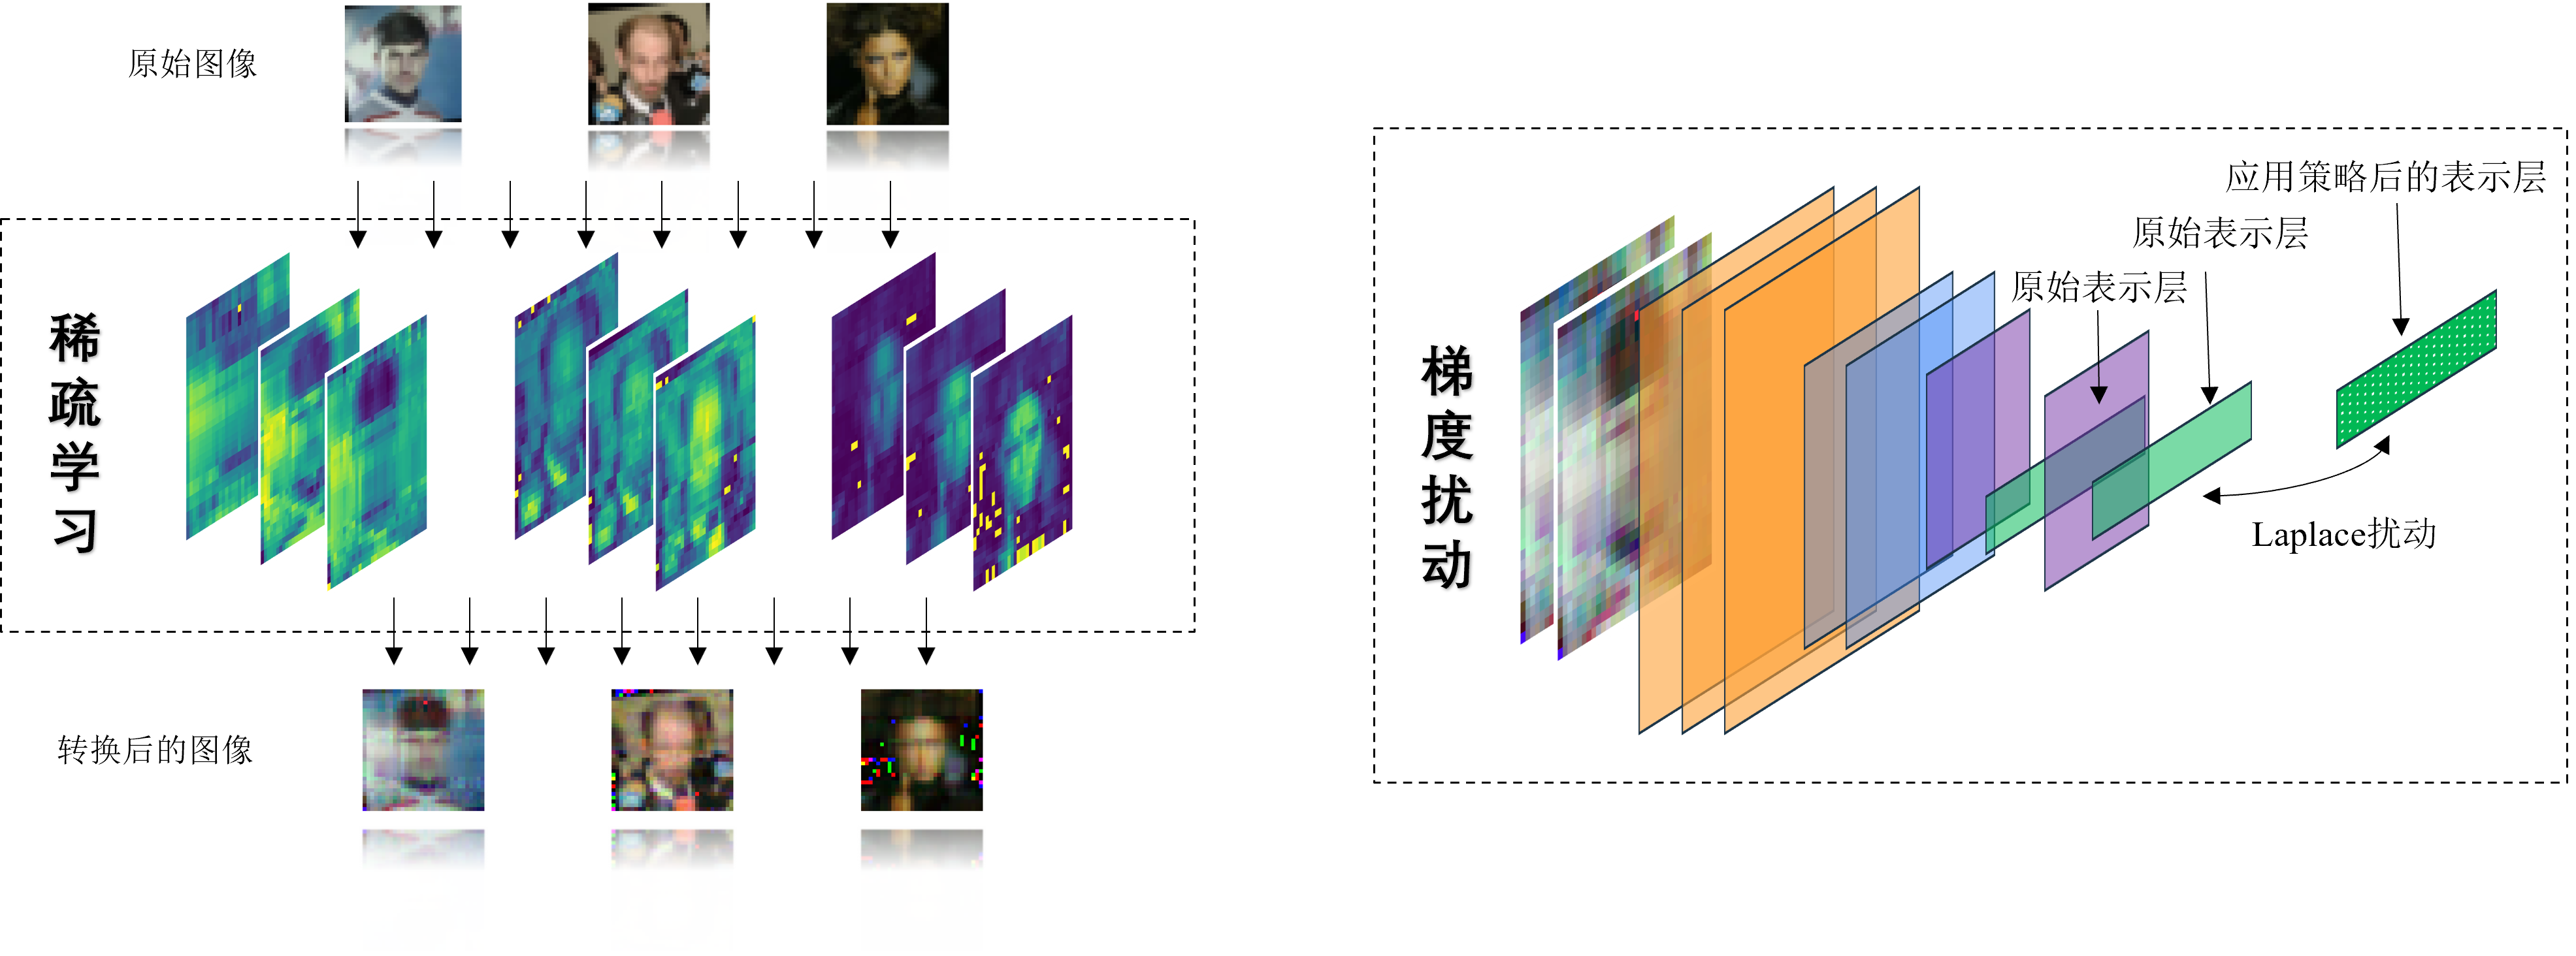
\includegraphics[scale=0.4]{figures/chapter4/chapter4.png}
    % \caption{FL-vgg16 Confusion Matrix}
    \caption{梯度泄露攻击的防御}
    \label{fig:Cluster the cars in the region}
\end{figure}

\subsection{梯度泄露攻击模型}

假设有一个神经网络$h_\theta:\mathbf{X}\to\mathbf{Y}$,使用参数$\theta$将输入空间$\mathbf{X}\subseteq\mathbb{R}^d$中的$x$映射到标签空间$\mathbf{Y}$中的$y$。假设输入$(x,y)$服从一个分布$\mathbf{D}$,则其边缘分布为$p(x)$。在本联邦学习系统中,有$n$个RSU,其各有一个损失函数$\mathbf{L}_1,\cdots,\mathbf{L}_n$,则要共同解决如下的优化问题:

\begin{equation}
\min_\theta\frac{1}{n}\sum_{i=1}^n\mathbb{E}{(x,y)\sim\mathbf{D}}\left[\mathbf{L}_i(h_\theta(x),y)\right]
\end{equation}

每一轮训练中,RSU$i$先在一组数据$(x_i,y_i)$上计算$\nabla_\theta \mathbf{L}_i(h_\theta(x_i),y_i)$,将其传给MEC。在MEC中使用一个梯度下降法,得到新的参数$\theta^{\prime}=\theta-\frac\alpha n\sum_{i=1}^n\nabla_\theta \mathbf{L}_i(h_\theta(x_i),y_i)$,$\alpha$是一个学习率。本节考虑一种情形,每个RSU上报的不是真实的梯度$\nabla_\theta \mathbf{L}_i(h_\theta(x_i),y_i)$,而是从分布$p(g|x)$中抽取的一个噪声梯度$g$,本节称之为防御机制。防御机制的目的是在梯度中加入足够的噪声,以掩盖用户的敏感信息,同时保留足够的信息量用于训练。因此,给定噪声梯度$g$,MEC将更新参数为$\theta^{\prime}=\theta-\frac\alpha n\sum_{i=1}^n g_i$。常见的防御例子是生成一个以截断的真实梯度为中心的噪声$p(g|x)$,比如在原始梯度上加上高斯(Gaussian)或拉普拉斯(Laplace)噪声,或者随机遮挡梯度的一些分量。$p(x)$和$p(g|x)$共同构成了一个联合分布$p(x,g)$。注意,没有防御的网络对应于分布$p(g|x)$,它只集中在$x$处的真实梯度上。

考虑一种场景,攻击者仅能观测到梯度 $g$,并试图从 $g$ 推断出产生它的输入 $x$。攻击者可以被视为一个函数 $f:\mathbb{R}^k\to \mathbf{X}$,其输入为梯度信息,输出一个重建的 $x$。设有一些 $(x,g)$ 的样本,它们服从联合分布 $p(x,g)$,则攻击者的重建 $f(g)$ 会导致一个损失 $\mathbf{L}'(x,f(g)):\mathbf{X}\times \mathbf{X} \to \mathbb{R}$。通常,采用一个二元损失,它仅在攻击者的重建和原始输入非常接近时为 $0$,否则为 $1$。若攻击者的目的是完全恢复输入 $x$,则损失可以定义为 $\mathbf{L}'(x,x^{\prime}):=\mathbf{O}_{x\neq x^{\prime}}$,其中 $\mathbf{O}$ 是指示函数。若攻击者的目的是找到输入 $x$ 在输入空间中的一个 $\delta$-邻域,则更适合的损失定义是 $\mathbf{L}'(x,x'):= \mathbf{O}_{d(x,x')>\delta}$,其中距离 $d$ 是 $\ell_{2}$ 距离。这种定义对于图像数据很有意义,因为 $\ell_{2}$ 距离能够反映人类对视觉相似度的感知,而且攻击者通常能够得到一个在视觉上或者在 $\ell_{2}$ 空间上都和原始图像很相似的重建。当 $\delta$ 趋近于 0 时,第二种损失定义就与第一种损失定义相同。基于此,可以定义攻击风险 $R(f)$ 为
\begin{equation}
\begin{aligned}
\frac{p_x(z)}{p_y(z)} &= \prod_{i=1}^{k} \frac{\exp\left(-\frac{e|f(x)_i - z_i|}{\Delta f}\right)}{\exp\left(-\frac{e|f(y)_i - z_i|}{\Delta f}\right)} \\
&= \prod_{i=1}^{k} \exp\left(\frac{e(|f(y)_i - z_i| - |f(x)_i - z_i|)}{\Delta f}\right) \\
& \leq \prod_{i=1}^{k} \exp\left(\frac{e(|f(x)_i - f(y)_i|)}{\Delta f}\right) \\
&= \exp\left(\frac{e \cdot ||f(x) - f(y)||_1 }{{\Delta f}}\right) \\
&\leq \exp(e)
\end{aligned}
\end{equation}


\subsection{基于稀疏学习的隐私保护策略}

本节的研究目标是找到一个转换函数$T$,使得每个原始输入$x$被转换为重构输入$\widehat{x}=T(x)$。因此,本节的研究目标可以分为以下两个方面:
\begin{itemize}
\item 目标 1:最小化重构输入和原始输入之间的相似度,以降低隐私泄漏风险。
\item 目标 2:最大化重构输入和原始输入表示的一致性,以保持FL的性能。
\end{itemize}

\subsubsection{隐私泄露得分$S_{pri}$}

针对目标1,本节引入隐私泄露得分$S_{pri}$,在\cite{Automatic_Transformation_Search_Against_Deep_Leakage_From_Gradients}的基础上加入攻击风险$R(f)$,用于衡量隐私信息泄露的程度,定义如下:
\begin{equation}
S_{pri}(T)=\frac{\gamma}{|\mathbb{R}|}\sum_{x\in \mathbb{R}} {Auc}(x,{\widehat{x}})+\beta{Var}_{T}+\delta R(f).
\end{equation}
为了简单起见,可以将这个得分近似为数值积分:
\begin{equation}
S_{pri}(T)\approx \frac{\gamma}{|\mathbb{R}|N}\sum_{x\in \mathbb{R}}\sum_{j=0}^{N-1}{CosSim}\bigg(x^{\prime}\bigg(\frac{j}{N}\bigg),{\widehat{x}}\bigg)+\beta{Var}_{T}+\delta R(f).
\end{equation}
其中$\gamma$,$\beta$,$\delta$分别是AUC面积(Area Under Curve)、方差和攻击风险的权重,$\gamma+\beta+\delta=1$,${x^{\prime}(i)}={(1-i)*x_{0}+i*\widehat{x}}$。

\begin{itemize}
    \item $ CosSim$:余弦相似度,用于衡量两个输入样本的梯度相似性,假设$x_{1},x_{2}$ 具有相同的标签$y$,当给定相同的模型参数$W$时:\begin{equation}  {CosSim}(x_{1}, x_{2}) = \frac{\langle \bigtriangledown W(x_{1}, y), \bigtriangledown W(x_{2}, y) \rangle }{|| \bigtriangledown W(x_{1}, y) || \cdot || \bigtriangledown W(x_{2}, y) ||}. \end{equation}$ {CosSim}$的范围是$[-1, 1]$,$-1$ 表示完全相反,$1$ 表示完全相同,$0$ 表示无关
    \item $ {Auc}$:$ {CosSim}$ 曲线下的面积,表示转换策略T在减少图像 $x$ 上的隐私泄露方面的有效性,一个好的转换策略会使得 $Auc$ 很小:\begin{equation}  {Auc}(x, {\widehat{x}}) = \int _{0}^{1}  {CosSim}(x^{\prime }(i), {\widehat{x}}) di. \label{eq:AUC}\end{equation}
    \item $ {Var}$:代表不同类别和样本之间$ CosSim$ 的方差,因为转换策略 $T$ 的 $ CosSim$ 值会随差异量大图像而变化,因此需要衡量转换策略$T$的整体效果,并保证数据集的隐私安全:\begin{equation}  {Var}= \frac{\Sigma _{x\in \mathbb{R}} ( {Auc}(x, {\widehat{x}}) - \bar{ {Auc}})^{2}}{|\mathbb{R}|}, \end{equation} $\bar{ {Auc}}$ 是 $\mathbb{R}$ 中所有样本的 AUC 得分的平均值。 $ {Var}_{T}$ 值越小,表示转换策略在抵抗重建攻击时,对不同类别的图像有一致的性能。
\end{itemize}

\subsubsection{准确度得分$S_{acc}$}

针对目标2,本节采用\cite{Neural_architecture_search_without_training}中的指标来量化策略对性能的影响。它根据经验评估了局部线性图与架构性能之间的相关性,并找出了能产生最佳性能的图。具体来说,准备一个随机初始化的模型$f$,以及由目标策略转换的一小批数据样本$\lbrace \widehat{x}_{n}\rbrace _{n=1}^{N}$。首先计算梯度雅可比矩阵,如下图所示:
\begin{equation} J = {\begin{pmatrix}\frac{\partial f}{\partial \widehat{x}_{1}}, & \frac{\partial f}{\partial \widehat{x}_{2}}, & \cdots & \frac{\partial f}{\partial \widehat{x}_{N}} \ \end{pmatrix}}^{\top }. \end{equation}
然后计算它的相关矩阵:
\begin{equation} \left(M_{J}\right)_{ i, j} = \frac{1}{N} \sum _{n=1}^{N}J_{i, n}, \ C_{J} = (J-M_{J})(J-M_{J})^{T}, \ \left(\Sigma _{J}\right)_{i, j} = \frac{\left(C_{J}\right)_{i, j}}{\sqrt{\left(C_{J}\right)_{i, i} \cdot \left(C_{J}\right)_{j, j} }}.  \end{equation}
令$\sigma _{J, 1} \leq \ldots \leq \sigma _{J, N}$ 为 $\Sigma_{J}$ 的 $N$个特征值。那么训练数据集中的准确率得分为
\begin{equation} S_{acc}(T)=\frac{1}{N}\sum _{i=0}^{N-1} {log(\sigma _{J,i} + \eta) + (\sigma _{J,i} + \eta)^{-1}},  \end{equation}

本节采用KSVD\cite{Deep_KSVD_Denoising}来实现转换函数$T$,用于其是一个低秩矩阵分解(Low-Rank Matrix Factorization)的问题,$\mathbf{X}$是一个给定的数据矩阵,$\boldsymbol{b}{j}$和$\boldsymbol{\omega}^{j}$是两组低秩矩阵,$k$是低秩的维度,$S_{pri}(T)$和$S_{acc}(T)$是两个优化目标函数,分别表示隐私保护(Privacy Protection)和准确性(Accuracy)的度量。一般来说,低秩矩阵分解的问题是非凸(Non-Convex)的,所以很难找到一个全局最优解。因此通常需要使用一些迭代算法(Iterative Algorithms),如梯度下降(Gradient Descent),交替最小二乘(Alternating Least Squares),或者随机梯度下降(Stochastic Gradient Descent),来逼近一个局部最优解。在这些算法中,$k$的取值会影响优化的结果和效率。一般来说,$k$越大,表示低秩矩阵的复杂度(Complexity)越高,能够更好地拟合数据矩阵$\mathbf{X}$,从而提高$S_{acc}(T)$的值。但是,$k$越大,也意味着低秩矩阵的稀疏性(Sparsity)越低,更容易泄露数据矩阵$\mathbf{X}$的信息,从而降低$S_{pri}(T)$的值。因此,$k$的取值需要在复杂度和稀疏性之间做一个平衡,以达到一个合理的折中方案。具体的$k$的取值,需要根据数据矩阵$\mathbf{X}$的特征,以及优化目标函数$S_{pri}(T)$和$S_{acc}(T)$的权重,算法流程如\ref{alg:Data sparsity algorithm}所示。

\begin{algorithm}[!th]
\caption{数据稀疏化}
\label{alg:Data sparsity algorithm}
\begin{algorithmic}[1]
    \REQUIRE 
        数据矩阵 $\mathbf{X}$, 低秩维度 $k$
    \ENSURE 
        转换函数 $T$, 重构输入 $\widehat{\mathbf{X}}$
    \STATE 初始化 $\widehat{\mathbf{X}} = T(\mathbf{X})$
    \STATE 初始化 $S_{pri}(T)$ 和 $S_{acc}(T)$
    \REPEAT
    % \STATE \textbf{functinon} Data\_sparsity\_algorithm()
        \FOR{each $j \in {1, \dots, k}$}
        \STATE Compute $S_{pri}(T')=\min(S_{pri}(T),\gamma{Auc}+\beta{Var}+\delta R(f))$
        \STATE Compute $S_{acc}(T')=\max(S_{acc}(T),\frac{1}{N}\sum _{i=0}^{N-1} {log(\sigma _{J,i} + \eta) + (\sigma _{J,i} + \eta)^{-1}})$
        \STATE Update $\widehat{\mathbf{X}}_j = T_j(\mathbf{X}_j)$
        \ENDFOR
        \STATE Update $\widehat{\mathbf{X}} = [\widehat{\mathbf{X}}_1, \dots, \widehat{\mathbf{X}}_k]$
    \UNTIL{收敛或达到最大迭代次数}
    \RETURN $T$
    % \STATE \textbf{end function}
    \end{algorithmic}
\end{algorithm}

\subsection{基于DP-SGD的梯度扰动策略}

联邦学习(FL)是一种分布式的机器学习方法,它允许多个参与者在本地使用自己的数据训练模型,然后将模型参数或更新信息发送给中心服务器,从而保护了用户数据的隐私。但是,这种方法仍然存在隐私泄漏的风险,因为数据表示层的信息可能会通过模型参数或更新信息泄露出去\cite{Soteria}。例如,恶意的参与者可以通过梯度信息,利用一些逆向工程的技术,重构出其他参与者的训练数据。为了解决这个问题,Gao等人\cite{Automatic_Transformation_Search_Against_Deep_Leakage_From_Gradients}提出了一种基于图像转换技术的隐私保护方案,它可以在保证模型性能的同时,有效地减少梯度信息的泄漏。然而,这种方案的一个缺点是,它会将一些扰动后的梯度设置为0,导致模型训练时的精度损失。因此,本节提出了一种改进的方案,将DP-SGD方案与梯度扰动方案结合,以实现更高效和更安全的隐私保护。

令$r$和$r^{\prime}$分别表示被防御层的干净数据表示和扰动数据表示。定义$x$和$x^{\prime}$为原始输入和通过扰动数据表示重构的输入。该方案的目标是在满足两个条件的情况下,最大化$x$和$x^{\prime}$之间的距离,以$L_2$范数衡量。这两个条件分别是:
\begin{itemize}
\item 目标1:$x$和$x^{\prime}$之间的距离应该尽可能大,以增加重构的难度和误差;
\item 目标2:$r$和$r^{\prime}$之间的距离应该有界,以保证扰动后的数据表示仍然能够保持模型的性能。
\end{itemize}
为了实现这个目标,该方案首先假设存在一个特征提取器$f:x\rightarrow r$,它可以将原始输入映射到数据表示层,以及它的逆函数$f^{-1}$,它可以将数据表示层映射回原始输入。进一步假设$f^{-1}$在$r$上是可微的,并且对于任意满足$||r-r'||_0\leq\epsilon$的$r'$,都有$f^{-1}(r')$存在。此外,根据链式法则,有$\nabla_{r}f^{-1}=(\nabla_{x}f)^{-1}$。基于这些假设,目标函数可以简化为:
\begin{equation}\begin{aligned}
&r^{\prime}\approx\arg\max_{r^{\prime}}\left\|\nabla_rf^{-1}\cdot(r-r^{\prime})\right\|_2,\mathrm{~s.t.~}\left\|r-r^{\prime}\right\|_0\leq\varepsilon\\
&=\arg\max_{r^{\prime}}\left\|\left(\nabla_xf\right)^{-1}\cdot\left(r-r^{\prime}\right)\right\|_2,\mathrm{~s.t.~}\left\|r-r^{\prime}\right\|_0\leq\varepsilon,
\end{aligned}\end{equation}
因此,该解决方案是在集合$\{||r_i(\nabla_xf(r_i))^{-1}||_2\}$中找到$\epsilon$个最大的元素,然后将它们对应的$r_i$作为扰动数据表示。这样,不仅可以提高重构的难度,还可以降低通信的开销,因为只需要传输非零的扰动数据表示。本文将其扩展到模型所有的表示层中,避免梯度冻结带来的防御策略失效现象,详细内容如算法\ref{alg:ImprovedDP-SGD}所示。

\begin{algorithm}[!htb]
\caption{改进版梯度扰动}
\label{alg:ImprovedDP-SGD}
\begin{algorithmic}[1]
\REQUIRE 数据矩阵 $\mathbf{X}$,损失函数$\nabla_\theta \mathbf{L}_i(h_\theta(\mathbf{X}),\mathbf{Y}))$,第$i$次迭代所需的学习率$\eta_i$, 噪声规模$\sigma$,组大小$\mathcal{G}$, 防御层之前的特征提取器$f: \mathbb{R}^{M \times N} \to \mathbb{R}^L$,干净的数据表示$r \in \mathbb{R}^L$,扰动边界$\epsilon$
\STATE 初始化 $\theta_{0}$
\FOR{each $i\in 1,\cdots,N$}
\STATE  在抽样概率 $q=\frac{\mathcal{G}}{n}$ 下随机抽样 $\mathcal{G}_i$。
\FOR{each $j\in \mathcal{G}_i$}
    \STATE \quad Compute $\widehat{\mathbf{x}}_j = T(x_j)$
    \STATE \quad Compute $g_i(x_j)=\nabla_\theta \mathbf{L}_j(h_\theta(\widehat{\mathbf{x}}_j),y_j)$
\ENDFOR

\FOR{each $j \in \text{Size}(g_i)$}
    \STATE \quad  提取$g_i$中的表示层,赋值索引为$k$
     \STATE \quad Compute $\mathbf{f}_i(r_k)=||r_k(\nabla_{\widehat{\mathbf{x}}_j}f(r_k)^{-1}||_{2}$
     \STATE \quad $\text{Find}\ \mathbf{f}_i$中$\epsilon$个最大元素的索引集合$S$
     \STATE \quad Set $r'_m=\zeta_{Lap},\text{if} \  m \in S$。
\ENDFOR
\STATE  $\theta_{t+1}=\theta_i-\eta_i g_i$
\ENDFOR
    % \STATE \textbf{end function}
\end{algorithmic}
\end{algorithm}

\section{基于稀疏学习和梯度扰动的梯度泄露防护实验}
\subsection{实验设置和实现细节}

% 数据集和模型。在不损失通用性的前提下,在两个数据集(CIFAR10\cite{cifar10}、Fashion MNIST(F-MNIST)\cite{Fashion-MNIST})和常规 LeNet 模型上验证提出方法的有效性。为了证明先进性,在三个数据集(LFW (Labeled Faces in the Wild)数据集\cite{LFW}、MNIST数据集、CIFAR-100数据集\cite{cifar10})和LeNet模型上,同其他方法方法进行横向对比。所有的数据集都按照8:2进行训练集和测试集的划分。

% 训练配置。实验在一台Ubuntu服务器上,其配置为Intel(R) Core(TM) i9-10980XE CPU @ 3.00GHz,GPU 型号是 TITAN RTX,这是一款高端的专业级显卡,它拥有 4608 个 CUDA 核心,24 GB 的 GDDR6 显存,672 GB/s 的显存带宽,16.3 TFLOPS 的单精度浮点性能,以及 130 TFLOPS 的张量核心性能。 采用带有动量、权重衰减和学习衰减技术的 SGD 优化器来保证全局模型的收敛性。具体而言,动量为 0.9、权重衰减为 $2\cdot 10^{-3}$ 的 SGD 来优化深度神经网络,批次大小都为200,对于梯度泄露防御以测试模型对隐私保护的防御能力是,训练历元设置为300轮,在进行图像分类以测试模型分类能力是训练50轮。

% 攻击实现。本章在实验中评估了两种攻击,以“优化器+距离测量”的格式命名。这些技术涵盖不同的优化器和距离度量:(1)采用LBFGS和L2范数进行优化的DLG(LBFGS+L2)\cite{DLG};(2)IG(adam+余弦)\cite{Inverting_Gradients},采用adam和余弦距离进行优化;

数据集和模型。本文提出了一种基于梯度泄露的隐私保护方法,为了验证其有效性和先进性,在两类数据集和一个经典的深度神经网络模型上进行了实验。这两类数据集分别是:(1)自然图像数据集,包括 CIFAR10\cite{cifar10}、CIFAR100\cite{cifar10} 和 Fashion MNIST(F-MNIST)\cite{Fashion-MNIST},它们包含了不同的图像类别和复杂度,可以用来测试模型的分类能力和鲁棒性;(2)人脸图像数据集 LFW (Labeled Faces in the Wild)数据集\cite{LFW},它包含了多个人脸的不同角度和表情,可以用来测试模型的识别能力和对抗性。选择 LeNet 作为深度神经网络模型,它是一个简单而有效的卷积神经网络,广泛应用于图像处理领域。将本文的方法与其他几种方法在这些数据集和模型上进行了横向对比,以展示所提出方法的优势和局限。为了保证实验的公平性,将所有的数据集都按照 8:2 的比例划分为训练集和测试集。

训练配置。实验环境是一台配置优良的 Ubuntu 服务器,其具体参数如下:处理器为 Intel(R) Core(TM) i9-10980XE CPU @ 3.00GHz,具有 18 个物理核心和 36 个逻辑核心,显卡为 TITAN RTX,拥有 4608 个 CUDA 核心,24 GB 的 GDDR6 显存,内存为 128 GB。本文使用 SGD 优化器来训练深度神经网络,这是一种常用的优化算法,可以有效地降低模型的损失函数。本文为 SGD 优化器设置了一些技术参数,以提高模型的收敛速度和稳定性,具体如下:动量为 0.9,可以加速模型的收敛方向和避免陷入局部最优;权重衰减为 $2\cdot 10^{-3}$,可以防止模型的过拟合和正则化模型的复杂度;学习率为 0.01,并且每 50 轮衰减为原来的 0.1,可以根据模型的训练进度动态地调整学习率的大小,以平衡模型的收敛速度和精度。本文将批次大小设置为 200,这意味着每次训练从训练集中随机抽取 200 个样本作为输入,以减少模型的内存占用和计算时间。本文根据不同的实验目的,设置了不同的训练轮数,具体如下:对于梯度泄露防御的实验,设置了 300 轮,以测试模型对隐私保护的防御能力;对于图像分类的实验,设置了 50 轮,以测试模型的分类能力。

攻击实现。为了评估本文提出方法的隐私保护效果,在实验中实现了两种常见的梯度泄露攻击,它们都是基于优化器和距离测量的方法,可以从模型的梯度中重构出原始的输入数据。这两种攻击分别是:(1)DLG(LBFGS+$L_2$)\cite{DLG},使用了 LBFGS 作为优化器利用历史信息来更新梯度方向和步长,从而加速优化过程;使用了 $L_2$ 范数作为距离测量,用于衡量两个向量之间的相似度,从而评估重构的质量;(2)IG(adam+余弦)\cite{Inverting_Gradients},使用了 Adam 作为优化器,根据梯度的变化情况动态地调整学习率和动量,从而适应不同的优化场景;使用了余弦距离作为距离测量,衡量两个向量之间的方向相似度,从而忽略向量的长度差异。本文将这两种攻击分别应用于所提出方法和其他几种方法,以比较它们的隐私保护性能和重构效果。

\subsection{策略的有效性评估}

本节提出的防御方法可以达到令人满意的变换策略。图\ref{fig:CIFAR10 with ours in DLG}展示了在 CIFAR10\cite{cifar10}和Fashion MNIST(F-MNIST)\cite{Fashion-MNIST}数据集的 DL 攻击 \cite{DLG} 下,使用和不使用策略重建图像的直观对比。观察到,在没有任何转换的情况下,攻击者可以非常高的保真度恢复图像(第 3 行 和 第 6 行)。相反,训练样本经过转换后(第 2 行和 第 5 行),攻击者几乎无法从恢复的图像中获得任何有意义的信息(第 4 行)。本节在其他数据集上(图\ref{fig:Defense strategy comparison experiment})也得到了类似的结果。

\begin{figure}[htb]
\centering
    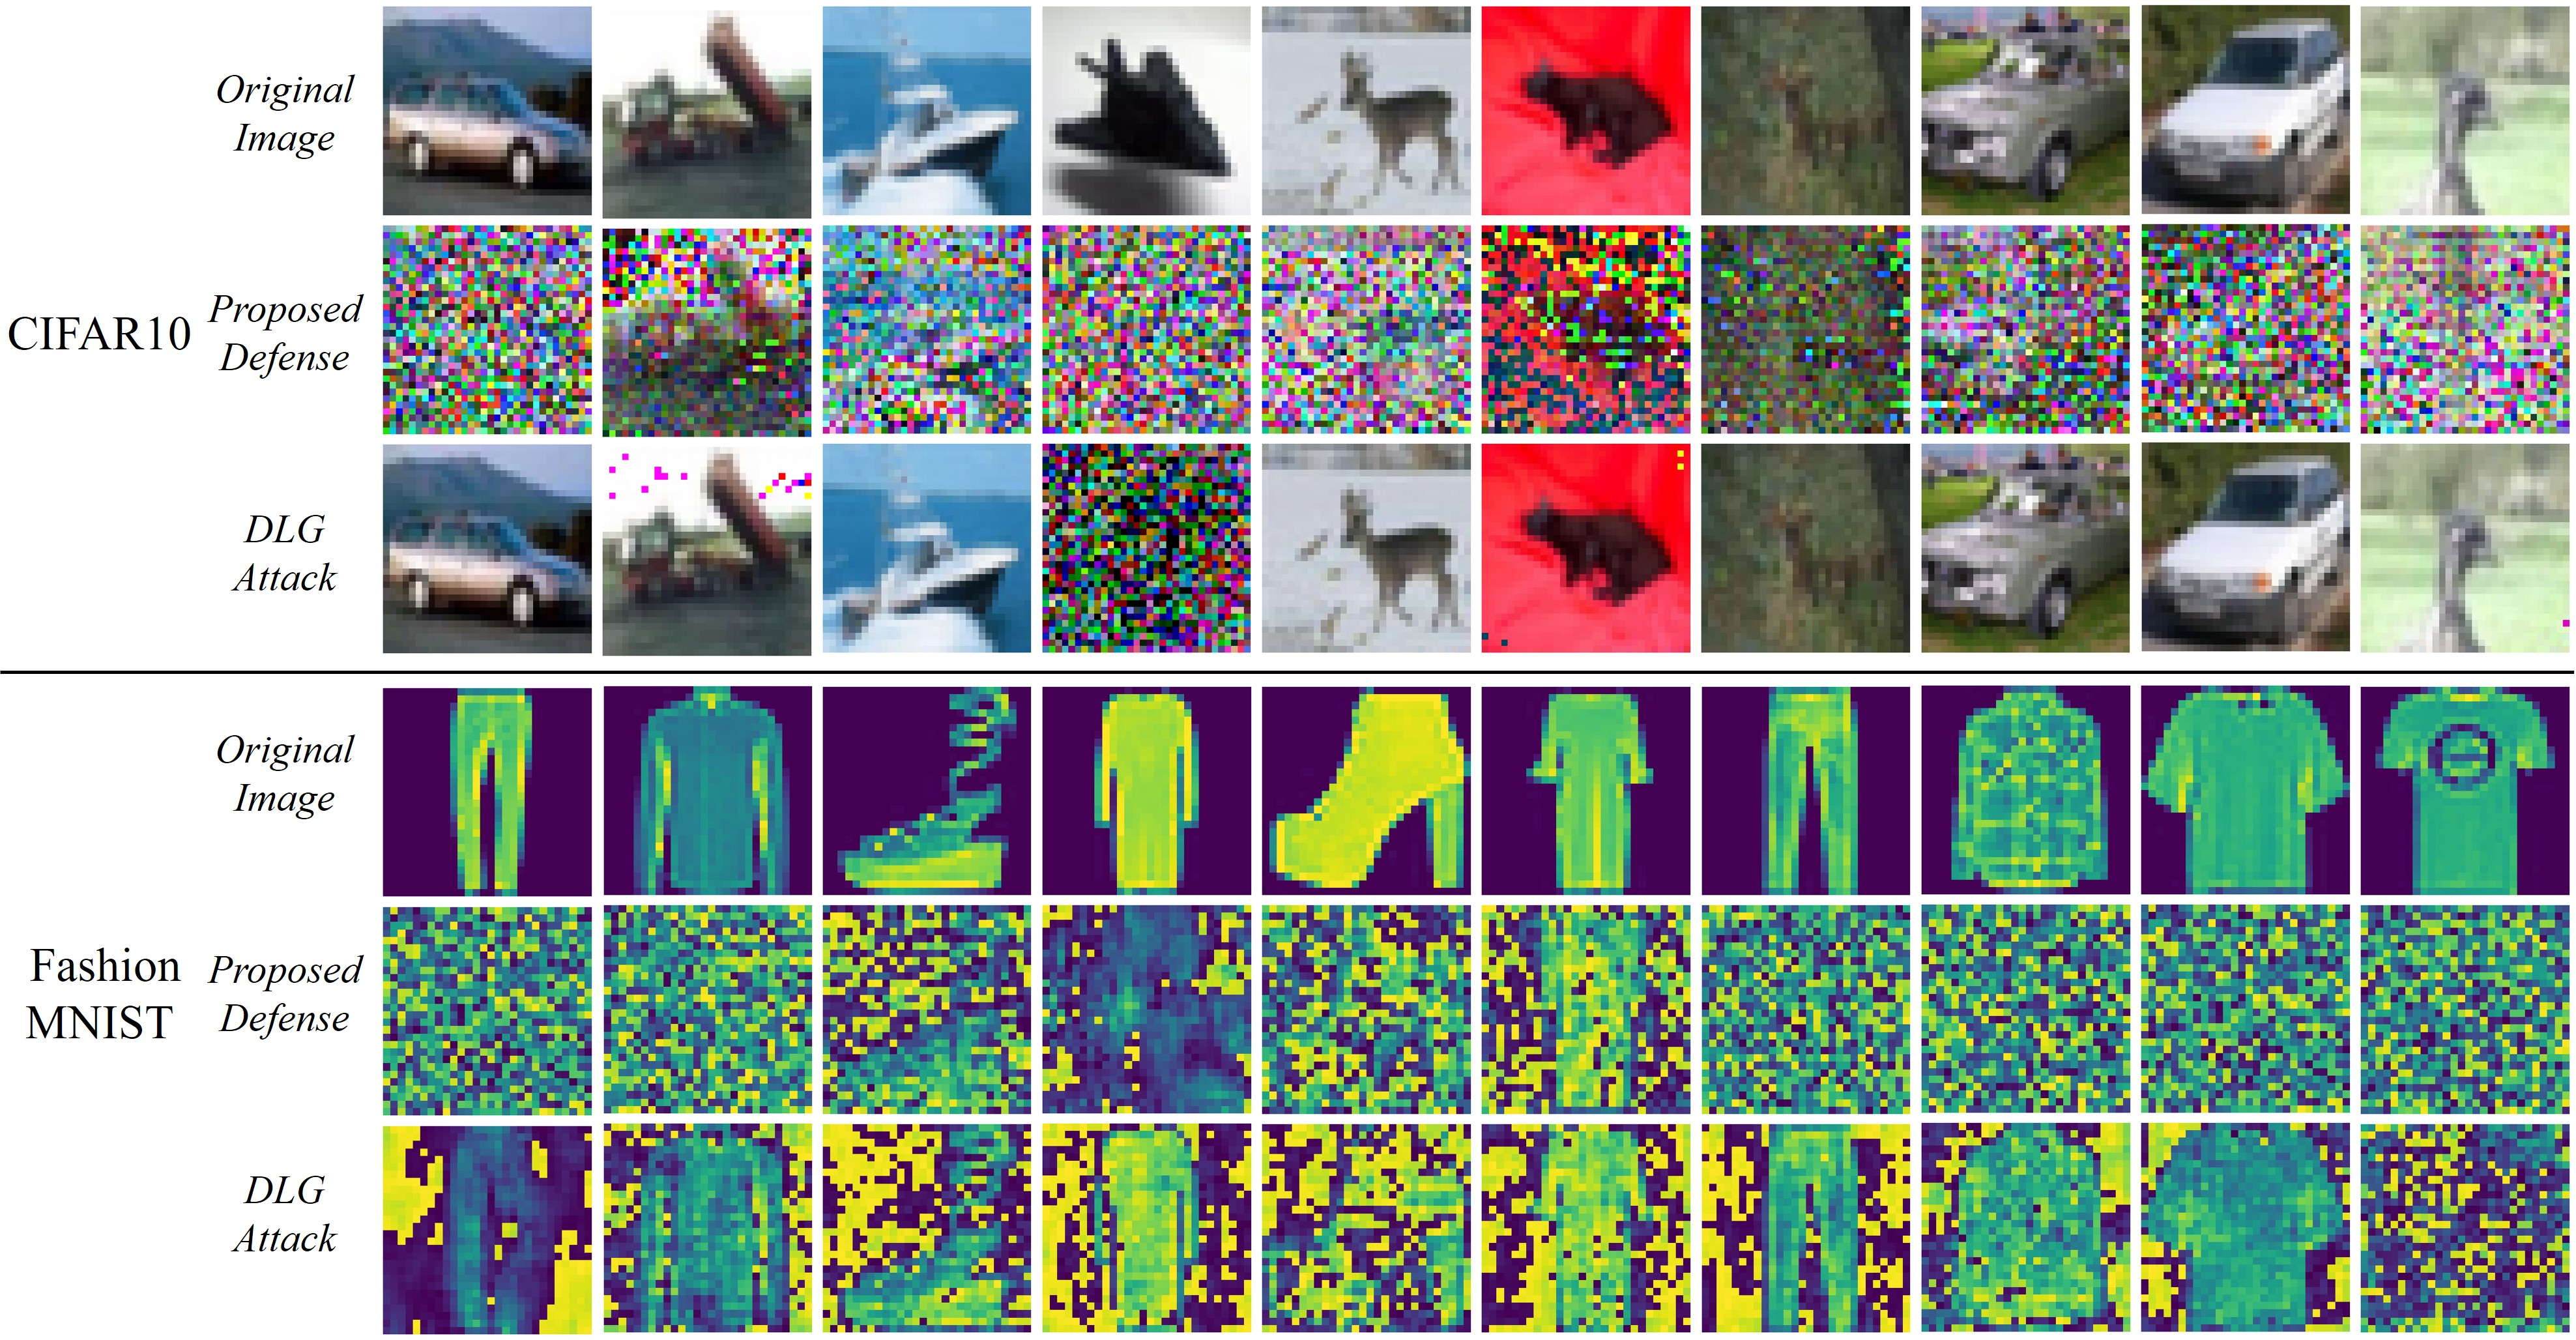
\includegraphics[scale=0.5]{figures/chapter4/Comparative experiment of strategy effectiveness.jpg}
    % \caption{FL-vgg16 Confusion Matrix}
    \caption{在CIFAR10和MNIST数据集上使用和未使用本节的防御方法进行重构攻击的可视化结果。第 1 行:原始样本,第 2 行:应用本节方法的样本,第 3 行:未使用任何防御。}
    \label{fig:CIFAR10 with ours in DLG}
\end{figure}

与其他防御方法的比较。为了评估本节提出的防御方法在不同数据集上的效果,本文将其与其他几种防御方法进行了对比,包括差分隐私(DP-Laplace 和 DP-Gaussian)、剪枝技术(GC)和 Sotria。本文使用了三个指标来衡量防御方法的性能,分别是 PSNR(峰值信噪比)、IIP-pixel(像素级逆向攻击指数)和 SSIM(结构相似性)。其中,PSNR 和 SSIM 越低,表示重构图像的质量越差,防御效果越好;IIP-pixel 越低,表示重构图像与原始图像的相似度越低,防御效果越好。图 \ref{fig:Defense strategy comparison experiment} 和表 \ref{tab:Defense strategy comparison experiment} 展示了在 LFW、MNIST 和 CIFAR-100 三个数据集上的对比结果。

\begin{figure}[htb]
    \centering
    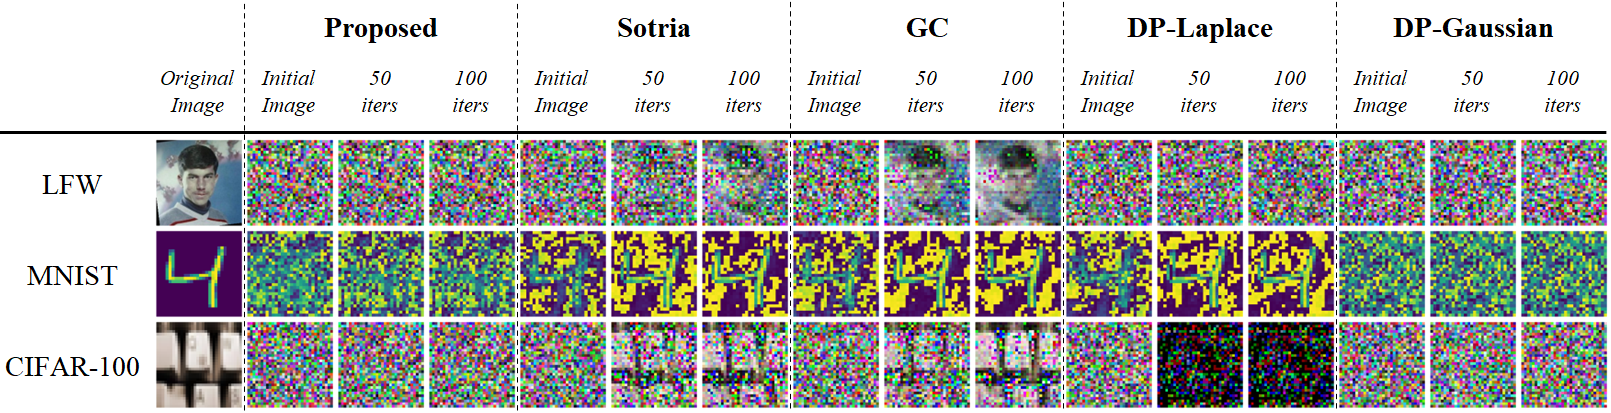
\includegraphics[width=1.0 \textwidth]{figures/chapter4/contrast experiment.png}
    \caption{本节的防御方法与其他防御方法在多个数据集上的对比结果}
     \label{fig:Defense strategy comparison experiment}
\end{figure}

从图 \ref{fig:Defense strategy comparison experiment} 中可以看出,本节的防御方法在所有数据集上都能显著降低 PSNR 和 SSIM 值,说明重构图像的质量很差,难以识别出原始图像的内容。从表 \ref{tab:Defense strategy comparison experiment} 中可以看出,本节的防御方法在所有数据集上都能达到最低的 IIP-pixel 值,说明重构图像与原始图像的相似度很低,难以进行像素级的逆向攻击。这些结果表明,本节的防御方法能有效地抵抗梯度泄露攻击,保护数据的隐私。相比之下,其他防御方法的效果都不理想。差分隐私方法虽然能降低 PSNR 和 SSIM 值,但是 IIP-pixel 值却很高,说明重构图像仍然保留了原始图像的一些特征,容易被逆向攻击。剪枝技术的效果更差,它几乎不能降低任何指标的值,说明重构图像的质量很高,与原始图像非常相似,没有达到防御的目的。Sotria 方法的效果也不稳定,它在某些数据集上能降低 PSNR 和 SSIM 值,但是在其他数据集上却反而提高了这些值,说明重构图像的质量与原始图像的复杂度有关,防御效果不一致。

\begin{table}[t]
\scriptsize
    \centering
    \begin{tabular}{lccccc}\hline
        &  & \textbf{LFW} & \textbf{MNIST} & \textbf{CIFAR-100} \\ \hline
        \multirow{3}{*}{\makecell{Proposed}}
        & PSNR & \textbf{10.620} & 10.014 & 8.935 \\
        & IIP-pixel & \textbf{0.318} &  \textbf{0.475} & \textbf{0.374} \\
        & SSIM & \textbf{0.431} &	\textbf{0.545} &	0.446 \\  \hline

        \multirow{3}{*}{\makecell{Sotria}}
        & PSNR &12.957 &	10.141 &	11.176  \\
        & IIP-pixel &0.343 &	0.552 &	0.491  \\
        & SSIM & 0.480 &	0.679 &	0.579  \\ \hline
        
        \multirow{3}{*}{\makecell{GC}}
        & PSNR & 18.609 &	9.460 &	12.424 \\
        & IIP-pixel & 0.369 &	0.513 &	0.523 \\
        & SSIM & 0.598 &	0.661 &	0.660 \\ \hline

        \multirow{3}{*}{\makecell{DP-Laplace}}
        & PSNR & 10.809 &	\textbf{9.413} &	\textbf{6.964} \\
        & IIP-pixel & 0.320 &	0.510 &	0.466 & \\
        & SSIM & 0.434 & 0.651 & \textbf{0.360}  \\ \hline
        
        \multirow{3}{*}{\makecell{DP-Gaussian}}
        & PSNR & 10.577 &	10.294 &	9.001 \\
        & IIP-pixel & 0.320 &	0.477 &	0.381 \\
        & SSIM & 0.432 &	0.536 &	0.448 \\ \hline
    \end{tabular}%
    \caption{\textmd{本节的防御方法与其他防御方法在多个数据集上的数值对比结果(取最后一轮结果)}}
    \label{tab:Defense strategy comparison experiment}
\end{table}

%此外,Sotria 方法还会导致模型的准确性明显下降,这是本节的防御方法所不具备的。综上所述,本节的防御方法在保持高模型准确性的同时,还能显著改善重构图像的质量,是一种有效的防御方法。

% \subsection{对模型性能影响}


\section{本章小结}

本节针对深度学习模型的梯度泄露攻击进行了详细的分析和研究,提出了一个基于稀疏学习和梯度扰动的梯度泄露防护的隐私保护策略。该策略主要包括两个方面:一是在模型训练的时候,利用基于稀疏矩阵的数据提取方案,将原始数据转化为稀疏化后的数据,从而降低数据的敏感性和可识别性;二是在模型训练过程中,对模型的所有表示层应用差分隐私与梯度扰动的隐私保护策略,通过在梯度上添加合适的噪声,防止梯度泄露攻击者利用梯度信息恢复出原始数据或模型参数。本节通过实验验证了该策略的有效性和模型性能影响,实验结果表明,本节提出的方案在隐私保护性和模型影响性方面都优于现有的流行方案,能够有效地抵御梯度泄露攻击,同时保持模型的高精度和泛化能力。
 								%第四章
	%  \setlength{\baselineskip}{20pt}
\chapter{总结与展望}
\label{cha:chap5}

论文的结论是最终的、总体的结论,不是正文中各段的小结的简单重复。结论应该准确、完整、明确、精练。如果不可能导出应有的结论,也可以没有结论而进行必要的讨论。可以在结论或讨论中提出建议、研究设想、仪器设备改进意见以及尚待解决的问题等。 								%第五章

	\nocite{*}
	\bibliography{reference/ref}

     \backmatter
	%\begin{appendix}
		%%% Local Variables:
%%% mode: latex
%%% TeX-master: "../main"
%%% End:

 \setlength{\baselineskip}{16pt}
\chapter{附录A}

%\section*{附录标题}
%\zihao{5}
%[内容为五号宋体。] 附录是作为论文主体的补充项目,并不是必须的。
%论文的附录依序用大写正体英文字母A、B、C……编序号,如:附录A。
%\vspace{0.75cm}
\begin{center}
\zihao{3}
\textbf{附录标题}
\end{center}



\indent
\zihao{5}
[内容为五号宋体。] 附录是作为论文主体的补充项目,并不是必须的。
论文的附录依序用大写正体英文字母A、B、C……编序号,如:附录A。
	%\end{appendix}

     %%% Local Variables:
%%% mode: latex
%%% TeX-master: "../main"
%%% End:

 \setlength{\baselineskip}{16pt}
\chapter{索引}



\indent
\zihao{5}
[内容为五号宋体。] 按照需要编排分类索引、著者索引、关键词索引等。 	

	%\mmchapter{作者简历}
 \setlength{\baselineskip}{16pt}
\chapter{作者简历及攻读硕士学位期间取得的研究成果}\zihao{5}
\setlength{\parindent}{0pt}

%[内容采用五号宋体]  包括教育经历、工作经历、攻读学位期间发表的论文和完成的工作等。行距16磅,段前后各为0磅。

一、作者简历

2009年,毕业于XX大学,XX学院,XX专业,获XX学士;

2009年至2010年,就读于XX大学,XX学院,XX专业,导师XX教授;

2010年至今,于XX大学,XX实验室,XX专业攻读博士学位,导师XX教授。

\vspace{10pt}
二、发表论文

[1] \textbf{XXX}, Truncated adaptation design for decentralized neural dynamic surface control of interconnected nonlinear systems under input saturation, \emph{International Journal of Control}, Volume 89, Issue 7, pp: 1447-1466, 2016. (SCI)\vspace{-5pt}

[2] \textbf{XXX},Clive Roberts, Lei Chen, Neural adaptive coordination control of multiple trains under bidirectional communication topology, \emph{Neural Computing and Applications}, Volume 27, Issue 8, pp: 2497-2507, 2016. (SCI)

[3] \textbf{XXX}, Neural adaptive control for uncertain MIMO systems with constrained input via intercepted adaptation and single learning parameter approach, \emph{Nonlinear Dynamics}, Volume 82, Issue 3, pp: 1109-1126, 2015. (SCI)


\vspace{10pt}
三、参与科研项目

[1]

[2]

[3]

\vspace{10pt}
四、专利

[1]

[2]

[3]


%\section*{访学经历}
%2011年8月至2011年11月,访问XX大学XX系,合作导师:XX教授;
%
%\section*{承担的科学研究工作}
%  (1) 主持,XX项目...。
%
%  (2) 参加,...;
%
%
%\section*{获奖情况}
%    
%    (1) 奖学金一等奖,北京交通大学,2016
%
%    (2) 博士研究生国家奖学金,中华人民共和国教育部,2013



	 \setlength{\baselineskip}{16pt}
\chapter{独创性声明}
%\thispagestyle{empty}


\zihao{5}

 
\hspace{2em}本人声明所呈交的学位论文是本人在导师指导下进行的研究工作和取得的研究成果,除了文中特别加以标注和致谢之处外,论文中不包含其他人已经发表或撰写过的研究成果,也不包含为获得北京交通大学或其他教育机构的学位或证书而使用过的材料。与我一同工作的同志对本研究所做的任何贡献均已在论文中作了明确的说明并表示了谢意。



\vspace{72pt}
 
\hspace{2em}学位论文作者签名:~~~~~~~~~~~~~~~~~~~~~~~~~~~~~~~~~~~~~~~~~~~签字日期:~~~~~~~~~~~~年~~~~~~~~月~~~~~~~~日 
 	

     
\chapter{学位论文数据集}\zihao{-4}


\setcounter{table}{0}
\renewcommand{\thetable}{1.\arabic{table}}

\begin{table}[!h]

\small 
\centering
\caption{数据集页}
\begin{tabular}{|p{2.6cm}|p{2.6cm}|p{2.5cm}|p{2.9cm}|p{2.5cm}|}
\hline
%\multirow{2}{*}{1} & \multicolumn{2}{|c|}{1} \\
%\cline{2-3}
%& 1 & 1 \\
%\hline
%1 & \multicolumn{2}{|c|}{1}\\
关键词$^*$  & 密级$^*$ & 中图分类号 & UDC & 论文资助 \\
\hline
         &   &            &     &          \\  %对应上一行的标题对应填写: 关键词、密级、中图分类号、UDC、论文资助
\hline

\multicolumn{2}{|p{5.4cm}|}{学位授予单位名称$^*$} & 学位授予单位代码$^*$ & 学位类别$^*$ &  学位级别$^*$    \\
\hline
\multicolumn{2}{|p{5.4cm}|}{北京交通大学 }        &  10004               &              &                  \\%对应上一行的标题对应填写: 学位类别、学位级别
\hline

\multicolumn{2}{|p{5.4cm}|}{论文题名$^*$} & \multicolumn{2}{p{5.4cm}|}{并列题名} &  论文语种$^*$    \\
\hline
\multicolumn{2}{|p{5.4cm}|}{   }          & \multicolumn{2}{p{5.4cm}|}{ }        &      \\ %对应上一行的标题对应填写: 论文题目、并列题名、论文语种
\hline

\ 作者姓名$^*$    &  \multicolumn{2}{p{5.4cm}|}{  }   & 学号$^*$  &     \\%在对应空格上填写:作者姓名,学号 
\hline

\multicolumn{2}{|p{5.4cm}|}{ 培养单位名称$^*$ }  &  培养单位代码$^*$   & 培养单位地址  &  邮编   \\
\hline
\multicolumn{2}{|p{5.4cm}|}{ 北京交通大学 }  &  10004   & 北京市海淀区西直门外上园村3号  &  100044   \\
\hline

\multicolumn{2}{|p{5.4cm}|}{ 学科专业$^*$ }  &  研究方向$^*$   & 学制$^*$  & 学位授予年$^*$   \\
\hline
\multicolumn{2}{|p{5.4cm}|}{  }              &                 &           &      \\%对应上一行的标题对应填写:学科专业、 研究方向、学制、学位授予年

\hline
论文提交日期 $^*$    & \multicolumn{4}{c|}{  }   \\%在对应空格上填写:论文提交日期 
\hline

\ 导师姓名$^*$    &  \multicolumn{2}{p{5.4cm}|}{  }   & 职称$^*$  &     \\%在对应空格上填写: 导师姓名、职称
\hline

\ 评阅人    &  \multicolumn{2}{p{5.4cm}|}{ 答辩委员会主席 }   & \multicolumn{2}{p{5.4cm}|}{ 答辩委员会成员 } \\
\hline
\        &  \multicolumn{2}{p{5.4cm}|}{   }   & \multicolumn{2}{p{5.4cm}|}{   } \\%对应上一行的标题对应填写:评阅人、主席、成员
\        &  \multicolumn{2}{p{5.4cm}|}{   }   & \multicolumn{2}{p{5.4cm}|}{   } \\
\        &  \multicolumn{2}{p{5.4cm}|}{   }   & \multicolumn{2}{p{5.4cm}|}{   } \\

\hline
\multicolumn{5}{|p{13.1cm}|}{ 电子版论文提交格式 \; 文本( )  图像( ) 视频( ) 音频( ) 多媒体( ) 其他( )}  \\
\multicolumn{5}{|p{13.1cm}|}{ 推荐格式:application/msword; application/pdf }  \\

\hline
\multicolumn{2}{|p{5.4cm}|}{ 电子版论文出版(发布)者  } & \multicolumn{2}{p{5.4cm}|}{电子版论文出版(发布)地  } & 权限声明\\
\hline
\multicolumn{2}{|p{5.4cm}|}{   } & \multicolumn{2}{p{5.4cm}|}{   } &  \\ %对应上一行的标题对应填写: 电子版论文出版(发布)者、发布地

\hline
论文总页数 $^*$    & \multicolumn{4}{c|}{  }   \\%在对应空格上填写:页数
\hline
\multicolumn{5}{|p{13.1cm}|}{ 共33项,其中带$*$为必填数据,为21项。 }  \\



\hline 
\end{tabular}	
\end{table}





















						


\end{document}




















